\documentclass[10.5pt, a4paper]{jreport} %jsreport

%\usepackage[margin=30truemm]{geometry}
\usepackage[top=25truemm,bottom=30truemm,left=30truemm,right=25truemm]{geometry}
\usepackage{fancyhdr}
\usepackage{abstract}
\usepackage{amsthm}
\usepackage{ulem}
\usepackage{setspace}
\usepackage{algorithm}
\usepackage{algpseudocode}
\usepackage{mathtools}
\usepackage{multirow}
\usepackage{amsmath,amssymb}
\usepackage{enumitem}
\usepackage{url}
\usepackage{bm}
\usepackage{pdfpages}
%\usepackage{algorithm2e}

\everymath{\displaystyle}

\def\thefootnote{\fnsymbol{footnote}}

\theoremstyle{definition}
\newtheorem{theorem}{定理}
\newtheorem{define}{定義}
\newtheorem{lemma}{補題}
\newtheorem{step}{Step}
\newtheorem*{counterexample}{反例}
\newtheorem{proposition}{命題}
\newtheorem{corollary}{系}

\renewcommand{\bibname}{参考文献}
\newcommand{\todayYMD}{\number\year 年\number\month 月\number\day 日}
\newcommand{\etodayMDY}{\ifcase\month\or
    January\or February\or March\or April\or May\or June\or
    July\or August\or September\or October\or November\or December\fi
    \space\number\day, \space\number\year}

% RequireとEnsureをInputとOutputにする
\renewcommand{\algorithmicrequire}{\textbf{入力:}}
\renewcommand{\algorithmicensure}{\textbf{出力:}}

\makeatletter
\renewcommand{\ALG@name}{アルゴリズム}
\makeatother

\renewcommand{\proofname}{\textbf{証明}}

\DeclarePairedDelimiter{\abs}{\lvert}{\rvert}

% 図表を並べるため
\makeatletter
\newcommand{\figcaption}[1]{\def\@captype{figure}\caption{#1}}
\newcommand{\tblcaption}[1]{\def\@captype{table}\caption{#1}}
\makeatother

%\pagestyle{fancy}
%\fancyhead{}
%\fancyhead[RO,RE]{\thepage}
%\fancyhead[LE,LO]{\leftmark}
%\cfoot{}
%\renewcommand{\chaptermark}[1]{\markboth{第\ \thechapter\ 章~#1}{}}

\begin{document}

% 表紙
\begin{titlepage}
  \begin{center}
    \vspace*{\stretch{1}}
    {\LARGE 修  士  論  文}\\
    \vspace{20truemm}
    {\Huge 線形無順序木パターンに対する\\グラフ畳み込みネットワークをオラクルとする質問学習モデル}\\
    \vspace{80truemm}
    {\LARGE 情報工学専攻}\\
    \vspace{10truemm}
    {\LARGE FM23102  石灘 洸樹}\\
    \vspace{10truemm}
    {\LARGE 指導教員  正代 隆義 教授}\\
    \vspace{20truemm}
    {\LARGE \todayYMD}
    \vspace{10truemm}\\
    {\LARGE 福岡工業大学 大学院}
    \vspace{\stretch{1}}
  \end{center}
\end{titlepage}
% ------------------------------

% 要旨
\input{00abst.tex}

% 目次用のページ番号
%\setcounter{page}{0}
%\pagenumbering{roman}
%\pagestyle{plain}

% 目次
\setcounter{tocdepth}{2} % subsection表示
\setcounter{page}{1}
\pagestyle{plain}
\setlength{\footskip}{10mm}
\tableofcontents
\pagebreak

% 行間調整
\begin{spacing}{1.3} % 横46x縦36

% 1 序論
% 1
%\chapter{序論}
\section{はじめに}
離散数学におけるグラフとは,頂点とそれらを結ぶ辺によって構成される基本的な数学的モデルの一つである.具体例としてグラフで表現できるデータには,都市間の移動や経路を視覚的に表現する路線図,化学物質における原子間の結合を示す分子構造モデル,さらにはウェブページやフォルダ構造の階層を表すHTMLやXMLの木構造などが挙げられる.これらのグラフは,単に接続性を示すだけでなく,情報科学,生物学,社会科学など多岐にわたる分野で,データ解析の基本となるものである.近年,これらのグラフに関連するデータ量は,情報通信技術の進展やビッグデータの普及に伴って飛躍的に増加しており,研究が活発に進められている.特に,グラフデータを活用した機械学習や深層学習の分野では,複雑な関係性をモデル化する手法が注目を集めている.その一つに,グラフ畳み込みネットワーク(Graph Convolutional Network: 以下,GCNと略す)がある.GCNは,従来の深層学習技術をグラフ構造に適用した手法であり,グラフデータが持つ構造的特徴を活用して学習を行う深層学習モデルである.具体的には,頂点や辺に付与された特徴量を,次数,ラベル,隣接関係などといった情報を考慮しながら,グラフ畳み込み層を通じて新たな特徴量を生成する仕組みを持つ.GCNの応用例としては,クラスタリング,ラベル推定,リンク予測などが挙げられる.このように,GCNは従来のグラフ理論と機械学習を融合させた強力なツールであり,グラフデータを扱う分野において特に注目されている.

質問学習モデルは,Angluin\cite{angluin-ml1988}によって提案された計算論的学習理論における機械学習モデルの一つである.このモデルは,常に正しい答えを返す教師(オラクル)を仮定し,機械学習における計算量などを解析するための数学的モデルである.具体的には,質問を通じて教師からのフィードバックを利用し,学習を進めるモデルである.特に,所属性質問や等価性質問を用いた文字列パターンの学習に関して,多くの理論的成果が得られている.例えば,文字列の正則パターン言語のクラスについて,1つの正例,すなわち文字列パターンにマッチする文字列を用いて多項式回数の所属性質問を行うことで,元の文字列パターンを同定可能であることが示されている\cite{angluin-jcss1980,angluin-ic1987}.ここで,所属性質問とは,与えられた文字列またはグラフが特定の言語やグラフ言語の要素であるか否かを問い合わせる質問を指す.Matsumotoら\cite{matsumoto-ieice2020}は,1つの正例とその長さ$N$の$O(N)$回の所属性質問を用いて正則パターン言語のクラスを同定する質問学習アルゴリズムを与えた.Uchidaら\cite{uchida2014,uchida-ieice2019}は,ある種のグラフ文法により生成可能な順序木構造パターン言語の質問学習可能性を詳細に議論した.これらの結果から,無順序木構造パターン言語のクラスに関しては,互いに異なる変数ラベルを持つ無順序木構造パターン言語のクラスが,1つの正例からそのサイズの多項式回数の所属性質問を用いて質問学習可能であることがわかる.また,所属性質問を用いて線形順序項木パターンに対する質問学習モデルに応用した例が小田ら\cite{oda-ai2022}により報告されている.彼らは,順序木データセットに対する二値分類問題において,著しく高い精度で計算するGCNを確認し,質問学習モデルを使用してGCNの予測根拠を可視化する手法を提案した.その手法は,順序木データに内在する複雑な構造的特徴を効率的に抽出し,それを基にした分類を可能にしている.

本論文では,常に正答を返す完全な教師(オラクル)を,高い精度で計算を行うGCNに置き換えることで,深層学習モデルと質問学習モデルを融合させた新しい協調モデルを導入する.この協調モデルは,従来の質問学習モデルが仮定していた完全なオラクルを使用せず,不完全な教師であるGCNを利用する点に特徴がある.不完全な教師を用いることで,現実的な問題設定における質問学習モデルの適用可能性を広げることができる.本モデルでは,GCNが木構造データから特徴を学習し,その結果をもとに質問学習を進めることで,データに内在する構造的特徴を抽出することを目指す.しかし,GCNは完全なオラクルとは異なり誤答を返す可能性がある.この協調モデルにより,データから効率的かつ効果的にパターンを発見し,質問学習の枠組みを深層学習モデルと統合する新たな可能性を示す.本論文において,無順序木データを用いた実験的解析により,この協調モデルの有効性を確認する.

ここでは,データに内在する構造的特徴を構造的変数として表現し,互いに異なる変数ラベルを持ち,葉のみに変数を持つ線形無順序木パターンを扱う.2つのクラスから構成される無順序木データベースを$S$とする.本論文では,このデータセット$S$を対象として以下の3つの計算問題を扱う.
\begin{enumerate}
  \item[(1)] 二値分類問題: データセット$S$に含まれる各無順序木の特徴量を用いて,データセット$S$を元の2つのクラスに分類する問題.
  \item[(2)] 無矛盾性問題: データセット$S$を元の2つのクラスに分類するための線形無順序木パターンが存在するか否かを決定する問題.
  \item[(3)] 可視化問題: 一般的にブラックボックスである深層学習モデルの予測根拠を,線形無順序木パターンを用いて明らかにする問題.
\end{enumerate}
これら3つの問題の関係性を図\ref{fig:relation}に示す.人工データを用いた評価実験を通じて,3つの問題における精度を解析することでGCNをオラクルとする質問学習モデルの有効性を示し,このモデルの精度向上手法と拡張可能性について議論する.

% 図1.1
\begin{figure}[tb]
  \centering
  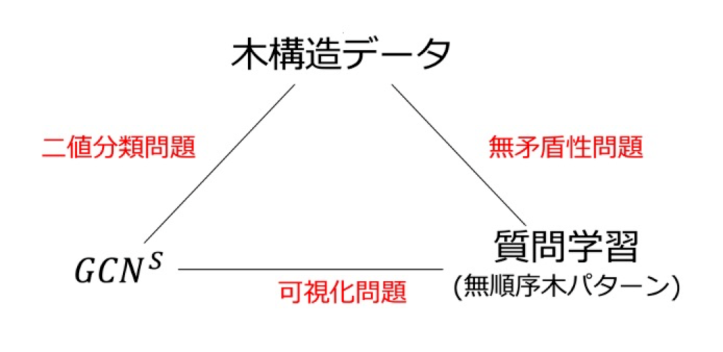
\includegraphics[scale=0.5]{fig/fig-relation.eps}
  \caption{データとモデルの関係性: 木構造データ$S$は無順序木の正例集合$S_+$と負例集合$S_-$の和集合である.$S$を訓練データとした学習済みGCNを$GCN^S$と記す.}\label{fig:relation}
\end{figure}

協調モデルを効率的に解析するために,1つのサイズ$N$の正例を入力とするとき,所属性質問を$O(N)$回用いる新たな質問学習アルゴリズムを提案し,その性能を実験的に評価する.このアルゴリズムは,少数の質問回数で正確な結果を得ることを目的としており,従来の手法に比べて効果的である.また,ある特定のグラフ畳み込み層と組み合わせることで高い精度を達成する.さらに,今後の研究の方向性として,順序木における構造のバランス化を通じた効率化を検討する.具体的には,順序木のバランス化を行うことで,その高さを抑制し,構造の深さに依存する処理を軽減することを目指す.このアプローチにより,特に木構造間のマッチング判定において,高速な解析が可能となることが期待される.この手法は,本論文が提案する質問学習アルゴリズムのさらなる発展の基盤となる.

%\section*{本論文の構成}
%第2章では,本論文の基礎となる内容として,グラフの基本的な用語,線形無順序木パターン,および線形順序項木パターンの定義について述べる.
%第3章では,線形無順序木パターンに対する質問学習モデルと所属性質問について述べ,無順序木パターンの無矛盾性問題がNP完全であることを証明する.その後,一つの正例とそのサイズに比例した回数の所属性質問を用いる新たな質問学習アルゴリズムを提案し,その正当性を理論的および実験的に示す.
%第4章では,オラクルとしてGCNを用いる質問学習モデルを定義し,その性能を実験的に評価する.
%第5章では,バランス化推論システムについて述べる.
%第6章では,本論文の結果をまとめるとともに,本研究の今後の課題について述べる.

% 2 準備
% 2
%\chapter{準備}
\section{準備}

% 2.1
\subsection{基本的用語}
集合$A$の$k$個の要素からなる部分集合の族を$[A]^k$で表す.グラフとは,$E\subseteq [V]^2$を満たす集合の組$G=(V,E)$のことである.$V$の要素をグラフ$G$の頂点と,$E$の要素を$G$の辺と呼ぶ.頂点$v$と辺$e$に対して,$v\in e$となるとき,$v$は$e$に接続するといい,$e$を$v$の接続辺と呼ぶ.1つの辺に接続する2つの頂点はその辺の端点と呼ぶ.頂点$v$の接続辺で$E$に属すもの全体の集合を$E(v)$で表す.グラフ$G$に辺$\{x,y\}$があるとき,$G$の2つの頂点$x,y$は隣接するといい,互いに他方の隣接点と呼ぶ.$G=(V,E)$と$G'=(V',E')$を2つのグラフとする.その頂点集合の間の全単射$\phi :V\rightarrow V'$で,全ての$x,y\in V$に対して$\{x,y\}\in E\Leftrightarrow \{\phi(x),\phi(y)\}\in E'$を満たすとき$G$と$G'$は同型であるという.$G\cup G'= (V\cup V',E\cup E'),G\cap G'= (V\cap V',E\cap E')$とおく.$G\cap G'=\emptyset$のとき$G$と$G'$は交わらない.$V'\subseteq V$かつ$E'\subseteq E$ならば,$G'$を$G$の部分グラフと呼ぶ.$G'\subseteq G$であり,$G'$が$x,y\in V'$となる辺$\{x,y\}\in E$をすべて含むとき,$G'$は$G$の誘導部分グラフであるという.頂点$v$の次数$d_G(v)$とは,$v$の接続辺の個数$|E(v)|$である.$G$が明らかなときは,$d_G(v)$を単に$d(v)$と記す.次数の最大値$\Delta (G)= \max \{d(v)\mid v\in V\}$を最大次数という.道とは次のように与えられる空でないグラフ$P=(V,E)$のことである.
\begin{align*}
  V & = \{x_0,x_1,\ldots,x_k\},\\
  E & = \{\{x_0,x_1\},\{x_1,x_2\},\ldots,\{x_{k-1},x_k\}\}\\
    & (x_i\neq x_j,0\leq i<j\leq k)
\end{align*}
$U$を任意の頂点(または辺)の集合とするとき,$G+U$は,$G$に$U$に属す頂点とその接続辺をすべて追加して得られるグラフである.$P$が道で,$k\geq 3$のとき,グラフ$C=P+\{\{x_{k-1},x_0\}\}$を閉路と呼ぶ.グラフ$G$に対して,その頂点集合を$V(G)$,辺集合を$E(G)$と記す.頂点の集合$A,B$に対して,$V(P)\cap A=\{x_0\}$かつ$V(P)\cap B=\{x_k\}$となるとき,$P=(x_0\ldots x_k)$を$A$-$B$道と呼ぶ.$A=\{x\},B=\{y\}$のとき,$A$-$B$道を単に$x$-$y$道と呼ぶ.2つの頂点$x,y$の距離$d_G(x,y)$とは,$G$における最短の$x$-$y$道の長さである.

% 2.2
\subsection{木}
グラフ理論において,木とはすべての頂点が連結しており,閉路(サイクル)を持たないグラフを指す.特に,根と呼ばれる頂点を1つ指定した木のことを\textbf{根付き木(rooted tree)}と呼ぶ.特別な注釈がない限り,本論文では木という用語は根付き木を意味するものとし,以降は根付き木を単に木と記述する.

$\Sigma$および$\Lambda$を有限アルファベット,$X$を無限アルファベットとする.ただし,$(\Sigma\cup\Lambda)\cap X=\emptyset$が成り立つものとする.また,頂点集合$V_T$と辺集合$E_T$を持つ木を$T = (V_T, E_T)$とする.$\{u,v\}\in E_T$に対して$u$が$v$より根に近いとき,辺$\{u,v\}$を順序対$(u,v)$で表す.以降,本論文では$(u,v)\in E_T$を$\{u,v\}\in E_T$かつ$u$が$v$より根に近いという意味で用いる.さらに,$(u,v)\in E_T$のとき,頂点$u$を$v$の親,$v$を$u$の子と呼ぶ.また,根ではない次数が1の頂点を葉と呼び,葉に接続する辺または変数を\textbf{葉辺(leaf edge)}と呼ぶ.木の頂点集合$V_T$の各頂点には$\Sigma$に属す記号が,辺集合$E_T$の各辺には$\Lambda$に属す記号がそれぞれラベル付けされているものとする.$\Sigma$に属す記号を頂点ラベル,$\Lambda$に属す記号を辺ラベルと呼ぶ.また,$X$に属す記号を変数ラベルと呼び,各$x \in X$にはランクと呼ばれる1以上の整数が割り当てられていると仮定する.

% 図2.1
\begin{figure}[tb]
  \centering
  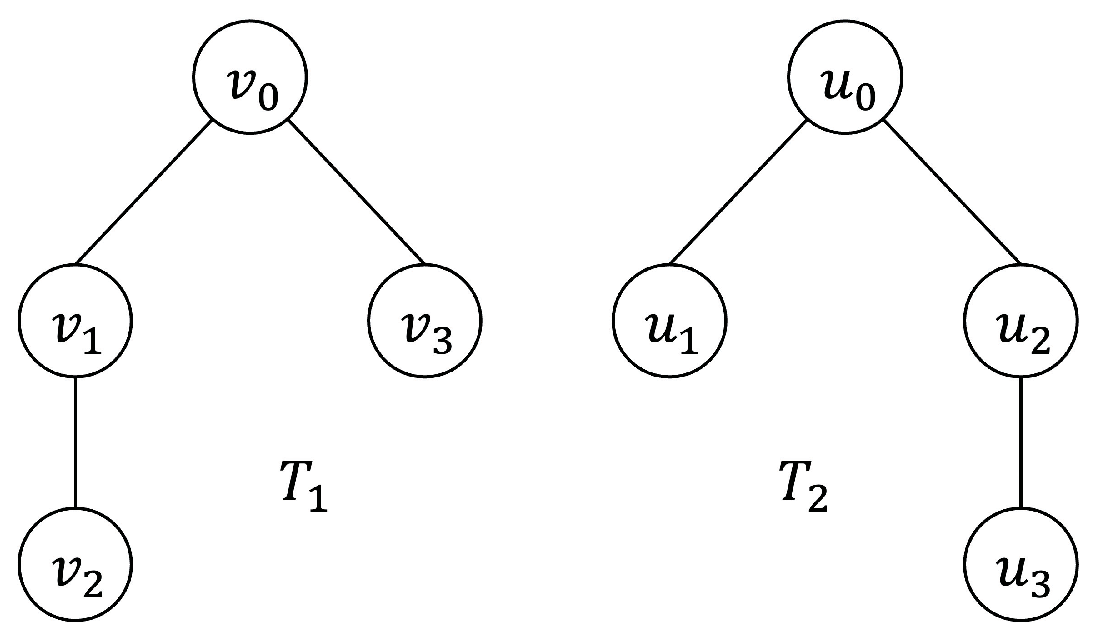
\includegraphics[scale=0.28]{fig-sibling_relationship.eps}
  \caption{$T_1$と$T_2$は,無順序木のときは同型,順序木のときは同型ではない.}\label{fig:sibling_relationship}
\end{figure}

% 2.3
% 無順序木パターン
% 2.3
\subsection{無順序木パターン}
\textbf{無順序木(unordered tree)}とは,後述する順序木と異なり同じ親を持つ頂点に順序関係(兄弟関係)を持たない木のことである.図\ref{fig:sibling_relationship}の2つの木は描き方は異なるが同じ木と扱われる.

% 定義1
\begin{define}{\bf 無順序木における変数}\par
  $\ell$を1以上の整数とする.$T=(V_T,E_T)$の変数とは,次の条件(1)--(3)を満たす$V_T$に含まれる頂点のリスト$h=[v_0,v_1,\ldots,v_{\ell}]$である.
  \begin{enumerate}
    \item[(1)] 頂点$v_0$は子を持つ.
    \item[(2)] $v_1,v_2,\ldots,v_{\ell}$ $(v_i \in V_T, 1\leq i\leq \ell)$は$v_0$の子である.% 順序木のときは「の連続した子である」
    \item[(3)] 変数$h$にはランクが$\ell+1$の変数ラベル$x\in X$がラベル付けされている.
  \end{enumerate}
  $v_0$を変数$h$の親ポート,$v_1,v_2,\ldots,v_{\ell}$を変数$h$の子ポートと呼ぶ.変数の次元とは,その変数に含まれる頂点数のことである.従って,変数$h=[v_0,v_1,\ldots,v_{\ell}]$の次元は$\ell+1$である.\par
  本論文では,変数を図\ref{fig:variable}のように四角で表す.四角に囲まれた文字は変数ラベルを表し,その変数が含む頂点を四角と数字付きの線で結ぶ.数字は変数におけるその頂点の順番を表す.線上の数字は,子ポートの数が1のときは省略する.
  図\ref{fig:variable}では変数ラベル$x$を持つ変数$h=[v_0,v_1,v_2,v_3]$を表す.$h$の次元は4である.
\end{define}

% 図2.2
\begin{figure}[tb]
  \centering
  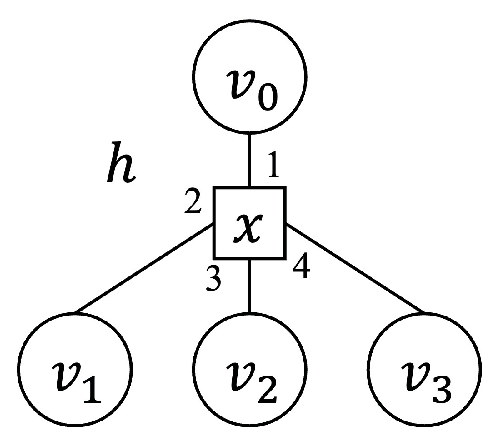
\includegraphics[scale=0.28]{fig-variable.eps}
  \caption{変数ラベル$x$を持つ変数$h=[v_0,v_1,v_2,v_3]$}\label{fig:variable}
\end{figure}

% 定義2
\begin{define}{\bf 無順序項木パターン(unordered term tree pattern)}\par
  $T=(V_T,E_T)$を無順序木とし,$H_T$を$T$の変数の集合とする.ただし,任意の異なる2つの変数$h_1,\,h_2\in H_T$に対して,$h_1$と$h_2$に共通して現れる頂点は高々1つであるとする.無順序項木パターンとは,次の条件(1)--(4)を満たす3つ組$t=(V_t,E_t,H_t)$である:
  \begin{enumerate}
    \item[(1)] $V_t=V_T$,
    \item[(2)] $E_t=E_T\setminus \left(\bigcup_{[v_0,v_1,\ldots,v_{\ell}]\in H_T}\{(v_0,v_i)\in E_T\mid 1\leq i\leq \ell\}\right)$,
    \item[(3)] $H_t=H_T$,
    \item[(4)] $V_t$に属す頂点の頂点ラベル,$E_t$に属す辺の辺ラベルは,それぞれに対応する$V_T$の頂点ラベル,$E_T$の辺ラベルと同じである.
  \end{enumerate}
\end{define}

% 定義2
\begin{define}{\bf 無順序項木パターンの束縛と代入}\par
  $x\in X$をランク$\ell+1$の変数ラベル,$g$を$\ell+1$個以上の頂点を持つ無順序項木パターンとする.$u_0$を$g$の根とし,$u_1,\ldots,u_{\ell}$を$g$の根以外の互いに異なる$\ell$個の頂点とし,$\sigma=[u_0,u_1,\ldots,u_{\ell}]$とする.このとき,形式$x:=[g,\sigma]$を$g$の$\sigma$による$x$への\textbf{束縛(binding)}または単に$x$の束縛という.
  $f=(V_{f},E_{f},H_{f})$を無順序項木パターンとする.ランク$\ell+1$の変数ラベル$x$を持つ変数が$f$に存在するとき,その変数を$h_1,\ldots,h_k$ $(k\geq 0)$とする.束縛$x:=[g,\sigma]$を変数$h_1,\ldots,h_k$に次のように同時に適用して得られる無順序項木パターンを$f\{x:=[g,\sigma]\}$と書く:
  \begin{enumerate}
    \item[(1)] $g_1,\ldots,g_k$を無順序項木パターン$g$と同型な無順序項木パターンとする.
    \item[(2)] 変数$h_j=[v_0^{(j)},v_1^{(j)},\ldots,v_{\ell}^{(j)}]$ $(1\leq j\leq k)$に関して,$H_f$から変数$h_j$を削除し,$g$の頂点$u_0,u_1,\ldots,u_{\ell}$に対応する$g_j$の頂点$u_0^{(j)},u_1^{(j)},\ldots,u_{\ell}^{(j)}$を,この順序で変数$h_j$の頂点$v_0^{(j)},v_1^{(j)},\ldots,v_{\ell}^{(j)}$と同一視する.同一視後の頂点ラベルは,頂点$v_0^{(j)},v_1^{(j)},\ldots,v_{\ell}^{(j)}$の頂点ラベルを継承する.
  \end{enumerate}
  \textbf{代入(substitution)}とは,$x_i\,(1\leq i\leq n)$が$X$の異なる変数ラベルであるような束縛の有限集合$\theta=\{x_1:=[g_1,\sigma_1],\ldots,x_n:=[g_n,\sigma_n]\}$である.
  ただし,$g_{1},\ldots,g_{n}$には変数ラベル$x_1,\ldots,x_n$を持つ変数が現れないと仮定する.
  代入$\theta$による$f$の\textbf{インスタンス(instance)}とは,$f$に対して,$\theta$の全ての束縛$x_i:=[g_i,\sigma_i]$ $(1\leq i\leq n)$を適用して得られる無順序項木パターンである.代入$\theta$による$f$のインスタンスを$f\theta$と書く.

  無順序木(順序木) $T_1$と$T_2$が無順序木(順序木)として同型であるとき,$T_1\equiv T_2$と書く.

  % 図2.3
  \begin{figure}[tb]
    \centering
    \includegraphics[scale=0.28]{fig-lutp.eps}
    \caption{線形無順序木パターン$t$と無順序木$t\theta \equiv T$を示す.無順序木の場合,代入後の$T$と下に示す$T_1,T_2,\ldots ,T_n$は同型である.}\label{fig:lutp} % 無順序木パターン$t$と無順序木$t\theta\equiv T$
  \end{figure}

  $\Sigma,\Lambda$をそれぞれ頂点ラベルの集合,辺ラベルの集合とする無順序木の全体を${\cal UT}_{\Sigma,\Lambda}$とする.また,$\Sigma,\Lambda,X$をそれぞれ頂点ラベルの集合,辺ラベルの集合,変数ラベルの集合とする無順序項木パターンの全体を${\cal UTTP}_{\Sigma,\Lambda,X}$とする.次のように${\cal UTTP}_{\Sigma,\Lambda,X}$の部分集合を定める:
  \begin{align*}
    {\cal LUTTP}_{\Sigma,\Lambda,X} & = \{t=(V_t,E_t,H_t)\in{\cal UTTP}_{\Sigma,\Lambda,X}\mid\\
    & \hspace*{12pt}\forall h_1,\,h_2\in H_t\,(h_1\not= h_2)\mbox{に対して,}\\
    & \hspace*{12pt}\mbox{変数}h_1\mbox{と}h_2\mbox{の変数ラベルは異なる}\},\\
    {\cal LUTP}_{\Sigma,\Lambda,X} & = \{t=(V_t,E_t,H_t)\in{\cal LUTTP}_{\Sigma,\Lambda,X}\mid\\
    & \hspace*{12pt}\forall h\in H_t\mbox{の次元は2であり,かつ}\\
    & \hspace*{12pt}\mbox{$h$の子ポートは葉である}\}.
  \end{align*}
  
  \noindent
  ${\cal LUTTP}_{\Sigma,\Lambda,X}$に属す無順序項木パターンを\textbf{線形無順序項木パターン(linear unordered term tree pattern)}と呼ぶ.また,${\cal LUTP}_{\Sigma,\Lambda,X}$に属す線形無順序項木パターンを\textbf{線形無順序木パターン(linear unordered tree pattern)}と呼ぶ.

  以降,無順序木$T=(V_T,E_T)$を,変数を持たない無順序項木パターン$T=(V_T,E_T,\emptyset)$とみなす.
\end{define}

% 定義4
\begin{define}{\bf 無順序項木パターン言語}\par
  無順序項木パターン$t\in {\cal UTTP}_{\Sigma,\Lambda,X}$に対して,$t$の無順序項木パターン言語$L(t)\subseteq {\cal UT}_{\Sigma,\Lambda}$を次のように定義する:
  $$L(t)=\{t\theta\in {\cal UT}_{\Sigma,\Lambda}\mid \mbox{$\theta$は$t$の変数への任意の代入}\}.$$
  \noindent
  線形無順序木パターン$t$に対して,$T\in L(t)$となる無順序木$T$の例を図\ref{fig:lutp}にあげる.
\end{define}


無順序項木パターン$t$と無順序木$T$に対して,代入$\theta$が存在して$t\theta\equiv T$となるとき,$t$は$T$にマッチするという.
%無順序項木パターン照合問題は次のように定義される決定問題である:
%
%\medskip
%\noindent
%\textbf{無順序項木パターン照合問題}(${\cal MP}$-${\cal UTTP}$)\\
%\textbf{入力}: 無順序項木パターン$t$と無順序木$T$;\\
%\textbf{問題}: $t$は$T$にマッチするか?
%\medskip
%
%上記問題と同様に,無順序項木パターンを線形無順序項木パターンに限定した\textbf{線形無順序項木パターン照合問題}(${\cal MP}$-${\cal LUTTP}$)を定める.無順序項木パターン照合問題は,$t$が線形無順序項木パターンであったとしても,次元4以上の変数が存在すればNP完全である\cite{shoudai-ieice2018}.一方,全ての変数の次元が2であれば,線形無順序項木パターン$t$に対する無順序項木パターン照合問題には入力サイズの多項式時間アルゴリズムが存在する\cite{shoudai-ieice2018}.従って,線形無順序木パターン$t\in{\cal LUTP}_{\Sigma,\Lambda,X}$に対する無順序項木パターン照合問題は入力サイズの多項式時間で計算可能である.
%無順序項木パターンに対する無矛盾性問題を次のように定義する.\par
%
%\medskip
%\noindent
%\textbf{無順序項木パターンに対する無矛盾性問題}(${\cal CP}$-${\cal UTTP}$)\\
%\textbf{入力}: 無順序木の有限集合$S_+\subseteq {\cal UT}_{\Sigma,\Lambda}$と$S_-\subseteq {\cal UT}_{\Sigma,\Lambda}$,ただし$S_+\cap S_-=\emptyset$.\\
%\textbf{問題}: $S_+\subseteq L(t)$かつ$S_-\cap L(t)=\emptyset$を満たす無順序項木パターン$t\in {\cal UTTP}_{\Sigma,\Lambda,X}$は存在するか?
%\medskip
%
%上記問題と同様に,無順序項木パターンを線形無順序項木パターンに限定した\textbf{線形無順序項木パターンに対する無矛盾性問題}(${\cal CP}$-${\cal LUTTP}$)を定める.Miyanoら\cite{miyano-ngc2000}は正規パターンに対して定義された無矛盾性問題がNP完全であることを示した.その結果から,${\cal CP}$-${\cal LUTTP}$がNP完全であることが導かれる.

% 定義5
\begin{define}{\bf 左深さ優先木}\par
  順序木において,左側の子を優先して深さ優先探索を行い,訪れた頂点の深さを並べた整数列を\textbf{深さ列(Depth Sequence)}と呼ぶ.順序木$T$における深さ列は$DS(T)$で表す.この深さ列は,木の構造における頂点の探索順序とその深さに基づいており,深さ優先探索における頂点訪問の順番を整数列として記録したものである.

  一方,無順序木の場合,子の順序が決まっていないため,子の順序を入れ替えることによって異なる順序木を構成することが可能である.無順序木においては,それと同型な様々な順序木表現が構成されるが,その中でも深さ列として辞書式順序で最大の値を持つものを\textbf{左深さ優先木(left depth first search tree)}と呼ぶ.この左深さ優先木がその無順序木を代表する順序木表現と考え,これを\textbf{左深さ優先無順序木(left depth first search unordered tree)}とする(図\ref{fig:left_dfs}).%左深さ優先木は,深さ優先探索において左側の子を優先的に探索するという特性を持つ.
  %具体的には,2つの無順序木が同型である場合,それらの左深さ優先木の深さ列は等しくなる.これは、無順序木の構造においてどのように子の順序を選んでも,左深さ優先木が持つ深さ列が唯一であることを意味している.
\end{define}

% 図2.4
\begin{figure*}[tb]
  \centering
  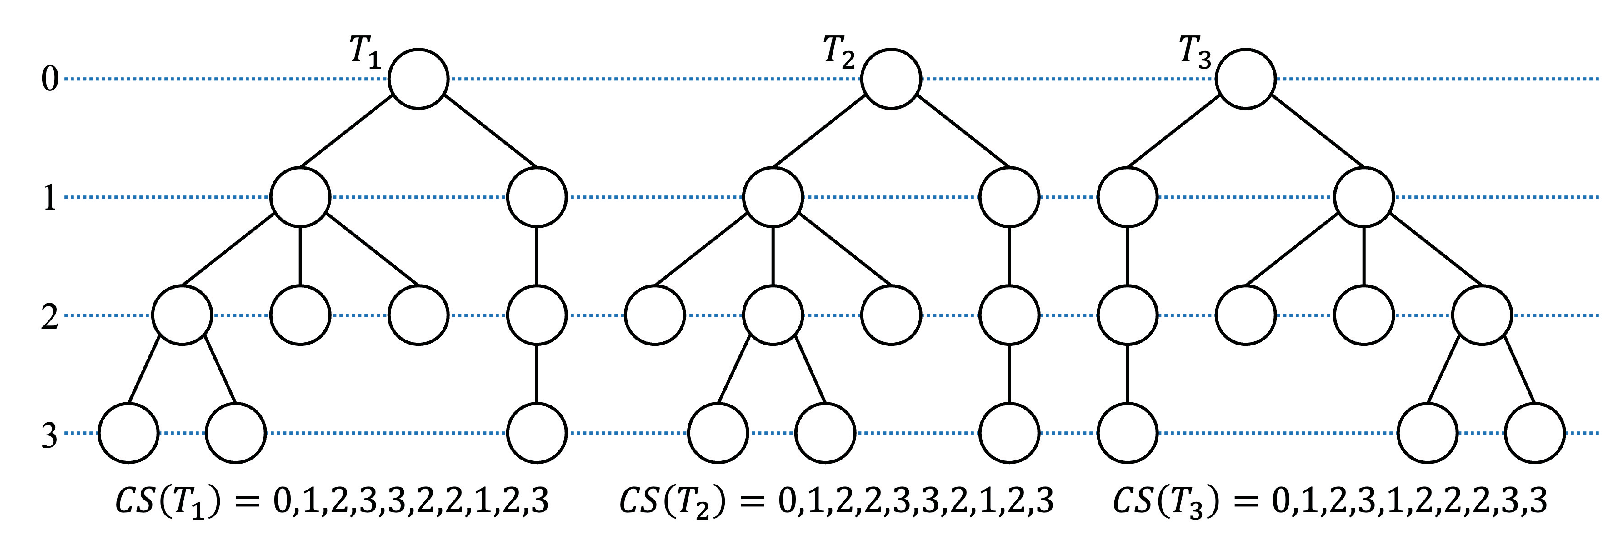
\includegraphics[scale=0.5]{fig-left_dfs.eps}
  \caption{$T_1,T_2,T_3$は同型の無順序木で,左深さ優先木を定めると$T_1$に一意に定まる.}\label{fig:left_dfs}
\end{figure*}

% 2.4
% 順序木
%% 2.4
\section{順序項木パターン}
\textbf{順序木(ordered tree)}とは,同じ親を持つ頂点に順序関係(兄弟関係)を持つ木のことである.順序木の例を図\ref{fig:sibling_relationship}に示す.これらの木は異なる木として扱われる.

% 定義6
\begin{define}{\bf 順序木における変数}\par
  $\ell$を1以上の整数とする.$T=(V_T,E_T)$を順序木とする.順序木$T$の変数とは,次の条件(1)--(3)を満たす$V_T$に含まれる頂点のリスト$h=[v_0,v_1,\ldots,v_{\ell}]$である.
  \begin{enumerate}
    \item[(1)] 頂点$v_0$は子を持つ.
    \item[(2)] $v_1,v_2,\ldots,v_{\ell}$ $(v_i \in V_T, 1\leq i\leq \ell)$は$v_0$の連続した子である.
    \item[(3)] 変数$h$にはランクが$\ell+1$の変数ラベル$x\in X$がラベル付けされている.
  \end{enumerate}
  無順序木における変数と同様に,$v_0$を変数$h$の親ポート,$v_1,v_2,\ldots,v_{\ell}$を変数$h$の子ポートと呼び,変数$h=[v_0,v_1,\ldots,v_{\ell}]$の次元を$\ell+1$とする.
\end{define}

% 定義7
\begin{define}{\bf 順序項木パターン(ordered term tree pattern)}\par
$T=(V_T,E_T)$を順序木とし,$H_T$を$T$の変数の集合とする.ただし,任意の異なる2つの変数$h_1,\,h_2\in H_T$に対して,$h_1$と$h_2$に共通して現れる頂点は高々1つであるとする.順序項木パターンとは,次の条件(1)--(4)を満たす3つ組$t=(V_t,E_t,H_t)$である:
\begin{enumerate}
  \item[(1)] $V_t=V_T$,
  \item[(2)] $E_t=E_T\setminus \left(\bigcup_{[v_0,v_1,\ldots,v_{\ell}]\in H_T}\{(v_0,v_i)\in E_T\mid 1\leq i\leq \ell\}\right)$,
  \item[(3)] $H_t=H_T$,
  \item[(4)] $V_t$に属す頂点の頂点ラベル,$E_t$に属す辺の辺ラベルは,それぞれに対応する$V_T$の頂点ラベル,$E_T$の辺ラベルと同じである.
\end{enumerate}
\end{define}

% 定義8
\begin{define}{\bf 順序項木パターンの束縛と代入}\par
  $x\in X$をランク$\ell+1$の変数ラベル,$g$を$\ell+1$個以上の頂点を持つ順序項木パターンとする.また,$u_0$を$g$の根とし,$u_1,\ldots,u_{\ell}$を$g$の根以外の互いに異なる$\ell$個の葉で,$u_i$が$u_{i+1}$ $(1\leq i\leq \ell-1)$より左の葉であるとき,$\sigma=[u_0,u_1,\ldots,u_{\ell}]$とする.このとき,形式$x:=[g,\sigma]$を$x$の\textbf{束縛(binding)}という.
  $f=(V_{f},E_{f},H_{f})$を順序項木パターンとする.ランク$\ell+1$の変数ラベル$x$を持つ変数が$f$に存在するとき,その変数を$h_1,\ldots,h_k$ $(k\geq 0)$とする.束縛$x:=[g,\sigma]$を変数$h_1,\ldots,h_k$に次のように同時に適用して得られる順序項木パターンを$f\{x:=[g,\sigma]\}$と書く:
  \begin{enumerate}
    \item[(1)] $g_1,\ldots,g_k$を順序項木パターン$g$と同型な順序項木パターンとする.
    \item[(2)] 変数$h_j=[v_0^{(j)},v_1^{(j)},\ldots,v_{\ell}^{(j)}]$ $(1\leq j\leq k)$に関して,$H_f$から変数$h_j$を削除し,$g$の頂点$u_0,u_1,\ldots,u_{\ell}$に対応する$g_j$の頂点$u_0^{(j)},u_1^{(j)},\ldots,u_{\ell}^{(j)}$を,この順序で変数$h_j$の頂点$v_0^{(j)},v_1^{(j)},\ldots,v_{\ell}^{(j)}$と同一視する.同一視後の頂点ラベルは,頂点$v_0^{(j)},v_1^{(j)},\ldots,v_{\ell}^{(j)}$の頂点ラベルを継承する.
  \end{enumerate}
  束縛による兄弟関係は,$f$と$g$の兄弟関係を拡張して定める\cite{suzuki-tcs2006}.
  \textbf{代入(substitution)}とは,$x_i\,(1\leq i\leq n)$が$X$の異なる変数ラベルであるような束縛の有限集合$\theta=\{x_1:=[g_1,\sigma_1],\ldots,x_n:=[g_n,\sigma_n]\}$である.
  ただし,$g_{1},\ldots,g_{n}$には変数ラベル$x_1,\ldots,x_n$を持つ変数が現れないと仮定する.
  代入$\theta$による$f$の\textbf{インスタンス(instance)}とは,$f$に対して,$\theta$の全ての束縛$x_i:=[g_i,\sigma_i]$ $(1\leq i\leq n)$を適用して得られる順序項木パターンである.代入$\theta$による$f$のインスタンスを$f\theta$と書く.

  $\Sigma,\Lambda$を頂点ラベルの集合,辺ラベルの集合とする順序木の全体を${\cal OT}_{\Sigma,\Lambda}$とする.また,$\Sigma,\Lambda,X$を頂点ラベルの集合,辺ラベルの集合,変数ラベルの集合とする順序項木パターンの全体を${\cal OTTP}_{\Sigma,\Lambda,X}$とする.次のように${\cal OTTP}_{\Sigma,\Lambda,X}$の部分集合を定める:
  \begin{eqnarray*}
  {\cal LOTTP}_{\Sigma,\Lambda,X} & = & \{t=(V_t,E_t,H_t)\in{\cal OTTP}_{\Sigma,\Lambda,X}\mid\\
  & & \hspace*{12pt}\forall h_1,\,h_2\in H_t\,(h_1\not= h_2)\mbox{に対して,$h_1$と$h_2$の変数ラベルは異なる}\}
  \end{eqnarray*}

  \noindent
  ${\cal LOTTP}_{\Sigma,\Lambda,X}$に属す順序項木パターンを\textbf{線形順序項木パターン(linear ordered term tree pattern)}と呼ぶ.

  以降,順序木$T=(V_T,E_T)$を,変数を持たない順序項木パターン$T=(V_T,E_T,\emptyset)$とみなす.
\end{define}

% 図2.5
\begin{figure}[tb]
  \centering
  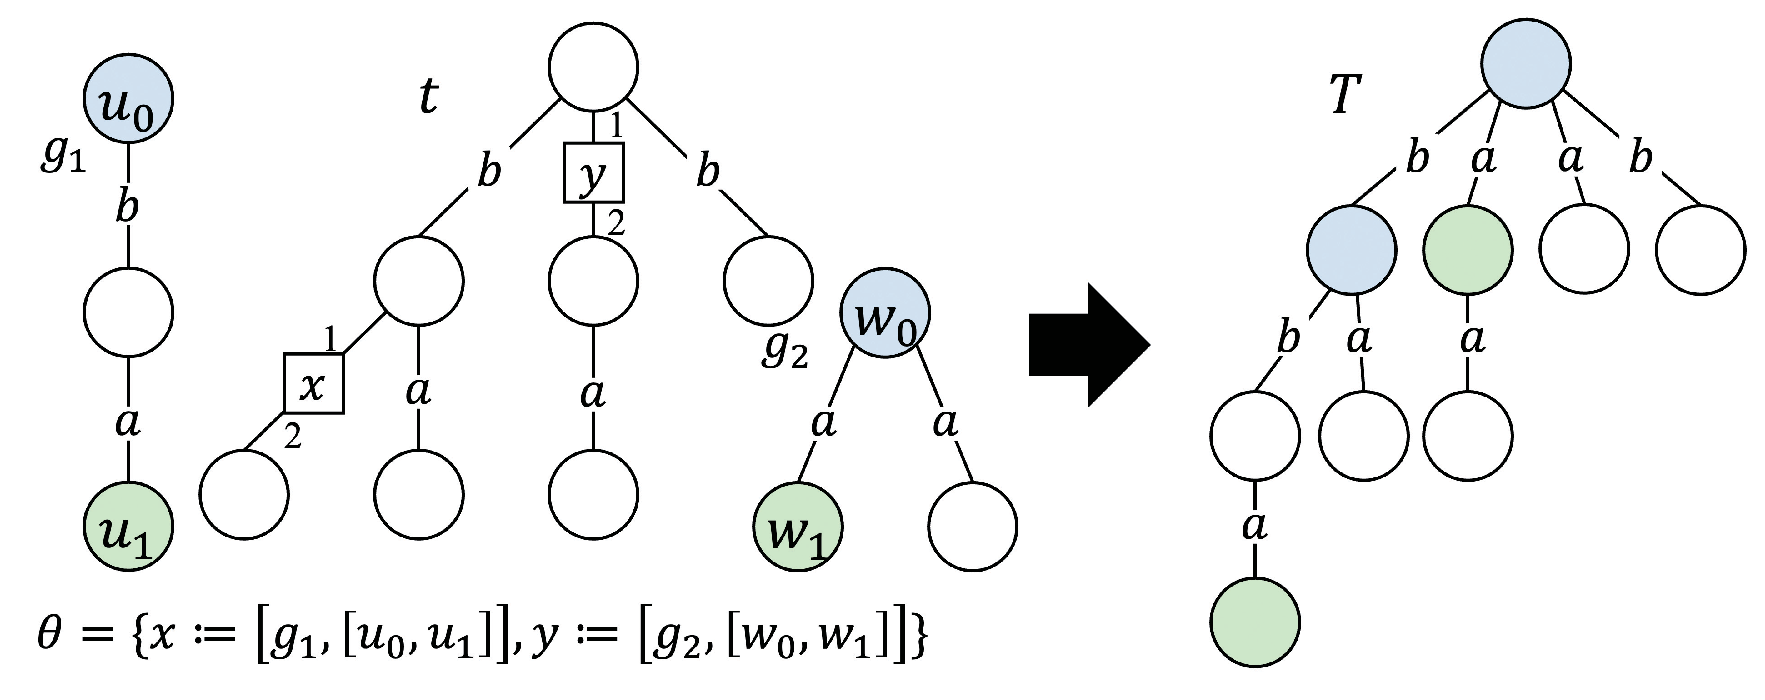
\includegraphics[scale=0.5]{fig-lottp.eps}
  \caption{線形順序項木パターン$t$と順序木$t\theta \equiv T$}\label{fig:lottp}
\end{figure}

% 定義9
\begin{define}{\bf 順序項木パターン言語}\par
  順序項木パターン$t\in {\cal OTTP}_{\Sigma,\Lambda,X}$に対して,$t$の順序項木パターン言語$L(t)\subseteq {\cal OT}_{\Sigma,\Lambda}$を次のように定義する:
  $$L(t)=\{t\theta\in {\cal OT}_{\Sigma,\Lambda}\mid \mbox{$\theta$は$t$の変数への任意の代入}\}.$$

  \noindent
  順序項木パターン$t$に対して,$T\in L(t)$となる順序木$T$の例を図\ref{fig:lottp}にあげる.
\end{define}

線形順序項木パターン$t$と順序木$T$に対して,$t\theta\equiv T$となるような代入$\theta$が存在するとき,$t$は$T$にマッチするという.線形順序項木パターン照合問題は次のように定義される決定問題である:

\medskip
\noindent
\textbf{線形順序項木パターン照合問題}(${\cal LOTTP}$-${\cal MP}$)\\
\textbf{入力}: 線形順序項木パターン$t$と順序木$T$.\\
\textbf{問題}: $t$は$T$にマッチするか?
\medskip

Suzuki et al.\cite{suzuki-tcs2006}は,線形順序項木パターン照合問題を解く$O(nN)$時間逐次アルゴリズムを提案した.$n$と$N$はそれぞれ線形順序項木パターン及び順序木の頂点数である.

% 2.5
% 質問学習モデル
% 2.5
\subsection{質問学習モデル}
質問学習モデルはAngluin\cite{angluin-ml1988}により提案された計算論的学習理論における機械学習モデルの一つである.質問学習モデルにおいては,学習対象に関する質問に正しく答えることができる完全な教師を仮定する.この教師の役割は,現実的には実現するのが難しい状況が多く,その意味で\textbf{オラクル(oracle)}と呼ぶ.学習対象に関する質問に対して,オラクルを仮定して計算量などの解析を行う.

質問学習モデルにおいて最もよく用いられる質問として所属性質問と等価性質問がある.学習対象の概念$C$に関する所属性質問とは「任意に与えられた要素$x$が$C$に属するか否か」を問い,$Yes$か$No$のどちらかで答えを受け取る質問である(図\ref{fig:ql}).等価性質問は,学習の過程で生徒が仮説$G$を見つけたとするとき,「$G$は正しい学習対象$C$と等しいですか?」と問い,もし等しければ$Yes$と,そうでなければその反例をひとつ受け取る質問である.

% 図2.6
\begin{figure}[tb]
  \centering
  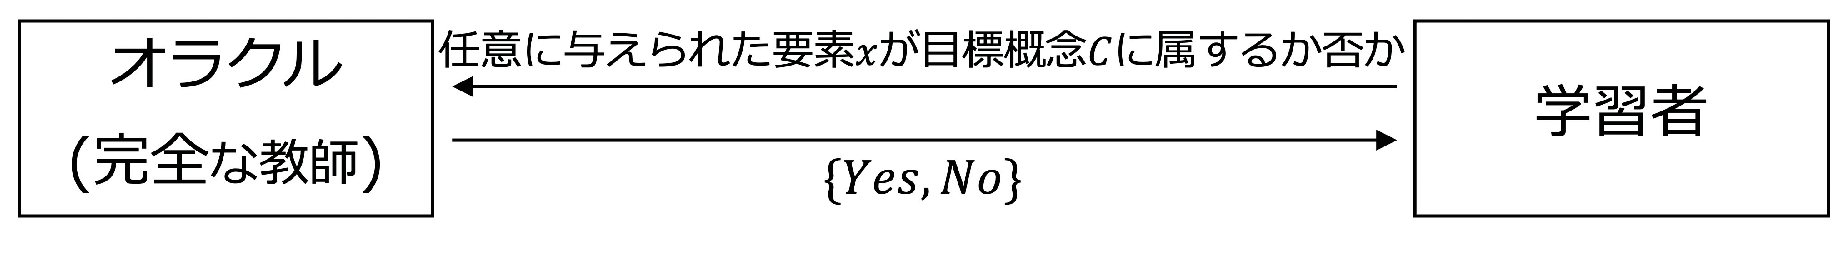
\includegraphics[scale=0.28]{fig-ql.eps}
  \caption{一般に学習対象の概念$C$に関する所属性質問}\label{fig:ql}
\end{figure}


% 3 理論的解析
% 3
%\chapter{線形無順序木パターンの質問学習}
\section{線形無順序木パターンの質問学習}

%2023年6月29日木曜日から7月1日土曜日まで沖縄科学技術大学院大学カンファレンス・センターにて行われた第143回数理モデル化と問題解決(MPS)と,2024年9月4日水曜日から9月6日金曜日まで広島工業大学五日市キャンパスにて行われた第23回情報科学技術フォーラム(FIT2024)で口頭発表を行った内容である.

% 3.1
\subsection{無順序木パターン言語の計算問題}
本章では,線形無順序木パターンの計算問題の時間計算量について述べる.
無順序項木パターン$t\in{\cal UTTP}_{\Sigma,\Lambda,X}$と無順序木$T=(V_T,E_T)$が与えられたとき,$T\in L(t)$か否かを決定する問題を次のように定義する.

\medskip
\noindent
\textbf{無順序項木パターン照合問題}(${\cal UTTP}$-${\cal MP}$)\\
\textbf{入力}: 無順序項木パターン$t\in {\cal UTTP}$と無順序木$T\in {\cal UT}$.\\
\textbf{問題}: $t$は$T$にマッチするか?
\medskip

無順序項木パターン照合問題は,$t$が線形無順序項木パターンであったとしても,次元4以上の変数が存在すればNP完全である\cite{shoudai-ieice2018}.
一方,全ての変数の次元が2であれば,無順序項木パターン$t\in {\cal UTTP}$と無順序木$T\in {\cal UT}$に対する無順序項木パターン照合問題は,$n$を$t$の頂点数,$N$を$T$の頂点数とするとき,$O(nN^{1.5})$時間で計算可能である\cite{shoudai-ieice2018}.従って,以下に示す線形無順序木パターン$t\in{\cal LUTP}_{\Sigma,\Lambda,X}$に対する無順序項木パターン照合問題は入力サイズの多項式時間で計算可能である.

\medskip
\noindent
\textbf{線形無順序木パターン照合問題}(${\cal LUTP}$-${\cal MP}$)\\
\textbf{入力}: 線形無順序木パターン$t\in {\cal LUTP}$と無順序木$T\in {\cal UT}$.\\
\textbf{問題}: $t$は$T$にマッチするか?
\medskip

次に,無順序項木パターン$t\in {\cal UTTP}$に対する無矛盾性問題を次のように定義する.

\medskip
\noindent
\textbf{無順序項木パターンに対する無矛盾性問題}(${\cal UTTP}$-${\cal CP}$)\\
\textbf{入力}: 無順序木の有限集合$S_+\subseteq {\cal UT}_{\Sigma,\Lambda}$と$S_-\subseteq {\cal UT}_{\Sigma,\Lambda}$,ただし$S_+\cap S_-=\emptyset$.\\
\textbf{問題}: $S_+\subseteq L(t)$かつ$S_-\cap L(t)=\emptyset$を満たす無順序項木パターン$t\in {\cal UTTP}_{\Sigma,\Lambda,X}$は存在するか?
\medskip

上記問題と同様に,無順序項木パターンを線形無順序項木パターン$t\in {\cal LUTTP}$に限定した\textbf{線形無順序項木パターンに対する無矛盾性問題}(${\cal LUTTP}$-${\cal CP}$)を次のように定める.

\medskip
\noindent
\textbf{線形無順序項木パターンに対する無矛盾性問題}(${\cal LUTTP}$-${\cal CP}$)\\
\textbf{入力}: 無順序木の有限集合$S_+\subseteq {\cal UT}_{\Sigma,\Lambda}$と$S_-\subseteq {\cal UT}_{\Sigma,\Lambda}$,ただし$S_+\cap S_-=\emptyset$.\\
\textbf{問題}: $S_+\subseteq L(t)$かつ$S_-\cap L(t)=\emptyset$を満たす線形無順序項木パターン$t\in {\cal LUTTP}_{\Sigma,\Lambda,X}$は存在するか?
\medskip

Miyanoら\cite{miyano-ngc2000}は正則パターンに対して定義された無矛盾性問題がNP完全であることを示した.次章で,${\cal LUTP}$-${\cal CP}$がNP完全であることを証明する.

% 3.2
\subsection{線形無順序木パターンに対する無矛盾性問題のNP完全性}
無順序木パターンは葉を子ポートとする次元2の変数しか現れない線形無順序項木パターンである.本章では,無順序木パターンの機械学習,特に二値分類問題に密接に関連する決定問題${\cal LUTP}$-${\cal CP}$がNP完全であることを証明する.

\medskip
\noindent
\textbf{線形無順序木パターンに対する無矛盾性問題}(${\cal LUTP}$-${\cal CP}$)\\
\textbf{入力}: 無順序木の有限集合$S_+\subseteq {\cal UT}_{\Sigma,\Lambda}$と$S_-\subseteq {\cal UT}_{\Sigma,\Lambda}$,ただし$S_+\cap S_-=\emptyset$.\\
\textbf{問題}: $S_+\subseteq L(t)$かつ$S_-\cap L(t)=\emptyset$を満たす無順序木パターン$t\in {\cal LUTP}_{\Sigma,\Lambda,X}$は存在するか?

以下では,$S_+$に属す無順序木を正例,$S_-$に属す無順序木を負例と呼ぶ.

% 定理1
\begin{theorem}
線形無順序木パターンに対する無矛盾性問題${\cal LUTP}$-${\cal CP}$はNP完全である.
\end{theorem}

\begin{proof}
線形無順序木パターンに対する無矛盾性問題がクラスNPに属すことは自明である.
NP完全であることが知られている充足可能性問題(3-SAT)から${\cal LUTP}$-${\cal CP}$への多項式時間帰着を示す.
$x_{1},\ldots,x_{n}$を$n$ $(n\geq 0)$個の論理変数とし,$x_{1},\ldots,x_{n}$の3つのリテラルからなる節を$C_{1},\ldots,C_{m}$ $(m\geq 0)$とする.
$F=C_{1}\vee\cdots\vee C_{m}$を3-CNFの論理式とする.
任意の$i$ $(1\leq i\leq n)$と$k$ $(1\leq k\leq m)$に対して,$C_{k}$はリテラル$x_i$と$\bar{x_i}$を両方とも含むことはないとしても一般性を失わない.
$F$が充足可能であるとき,そのときに限り,${\cal LUTP}$-${\cal CP}$の問題における条件を満たす線形無順序木パターン$t\in {\cal LUTP}_{\Sigma,\Lambda,X}$が存在するように$S_{+}$と$S_{-}$を構成する.
頂点ラベル,辺ラベルの集合をそれぞれ$\Sigma=\{\varepsilon\}$, $\Lambda=\{0,1,2,\textrm{a},\textrm{b}\}$とする.ここで,$\varepsilon$は空語を表す.
$T$を図\ref{fig:sample-tree}に定める最大深さ$n+1$の無順序木とする.
\begin{enumerate}
\item[(1)] 論理変数$x_{i}$ ($1\leq i\leq n$)に対する無順序木の正例$T_{i}^{(+)}$と負例$T_{i}^{(-)}$ $(1\leq i\leq n)$を次のように構成する:
$T$の深さ$i+1$ $(1\leq i\leq n)$の同じ親を持つ深さ$i+2$の3つの葉のうち,$0$を親への辺の辺ラベルとする葉を削除して得られる無順序木を$T_{i}^{(+)}$ ($1\leq i\leq n$)とする.また,$T$の深さ$i+1$ $(1\leq i\leq n)$の同じ親を持つ深さ$i+2$の3つの葉のうち,$1$または$2$を親への辺の辺ラベルとする葉の1つを削除して,他方の辺ラベルを$0$に変更して得られる無順序木を$T_{i}^{(-)}$ ($1\leq i\leq n$)とする(図\ref{fig:sample-tree}).
$T_{i}^{(+)}$の深さ$i+1$における葉のうち,親への辺の辺ラベル$1$は$x_{i}$の値が$true$であることを,親への辺の辺ラベル$2$は$x_{i}$の値が$false$をあることを表す.
線形無順序木パターン$t$で,$T_{i}^{(+)}\in L(t)$かつ$T_{i}^{(-)}\not\in L(t)$となるものが存在するならば,深さ$i+2$の葉に繋がる辺の辺ラベルによって,$L(t)$に属する無順序木か否かが判断されることに注意する.
なぜなら,$T_{i}^{(+)}$と$T_{i}^{(-)}$の違いは深さ$i+2$の葉に繋がる辺の辺ラベルだけであるからである.
さらに,$T_{i}^{(-)}$の深さ$i+1$の葉の親への辺の辺ラベルが$0$であることから,線形無順序木パターン$t$の深さ$i+1$の葉の親への辺には,辺ラベル$1$または$2$を持つものが存在しなければならない.
\item[(2)] 節$C_{k}$ ($1\leq k\leq m$)に対する無順序木を次のように構成する:
節$C_k$ $(1\leq k\leq m)$が論理変数$x_p,x_q,x_r$ $(1\leq p < q < r \leq n)$のリテラルを含むとき,$T$の深さ$p+1,q+1,r+1$の葉を次のように変更して,負例$T_{n+k}^{(-)}$ $(1\leq k\leq m)$を作成する(図\ref{fig:clause-tree}): $C_k$が含む論理変数$x_p$に対して,$T$の深さ$p+1$の同じ親を持つ3つの葉のうち,$0$を親への辺の辺ラベルとする葉を削除して,$x_p$が正のリテラルのとき,残りの2つの葉の親への辺の辺ラベルを両方とも$2$に,$x_p$が負のリテラルのとき,残りの2つの葉の親への辺の辺ラベルを両方とも$2$にする.$x_q$と$x_r$のリテラルに対しても,$T$の深さ$q+1$と$r+1$の葉に対して同様の操作を行う.このようにして構成した無順序木$T_{n+k}^{(-)}$ $(1\leq k\leq m)$は,$C_{k}$に含まれるリテラルが同時に$false$にならないことを表す.
\end{enumerate}
$S_{+}=\{T_1^{(+)},T_2^{(+)},\ldots,T_n^{(+)}\}\subseteq {\cal UT}_{\Sigma,\Lambda}$,$S_{-}=\{T_1^{(-)},T_2^{(-)},\ldots,T_{n}^{(-)}\}\cup\{T_{n+1}^{(-)},\ldots,T_{n+m}^{(-)}\}\subseteq {\cal UT}_{\Sigma,\Lambda}$とする.図\ref{fig:example_npc}に例をあげる.

\medskip

% 図3.1
\begin{figure}[tb]
  \centering
  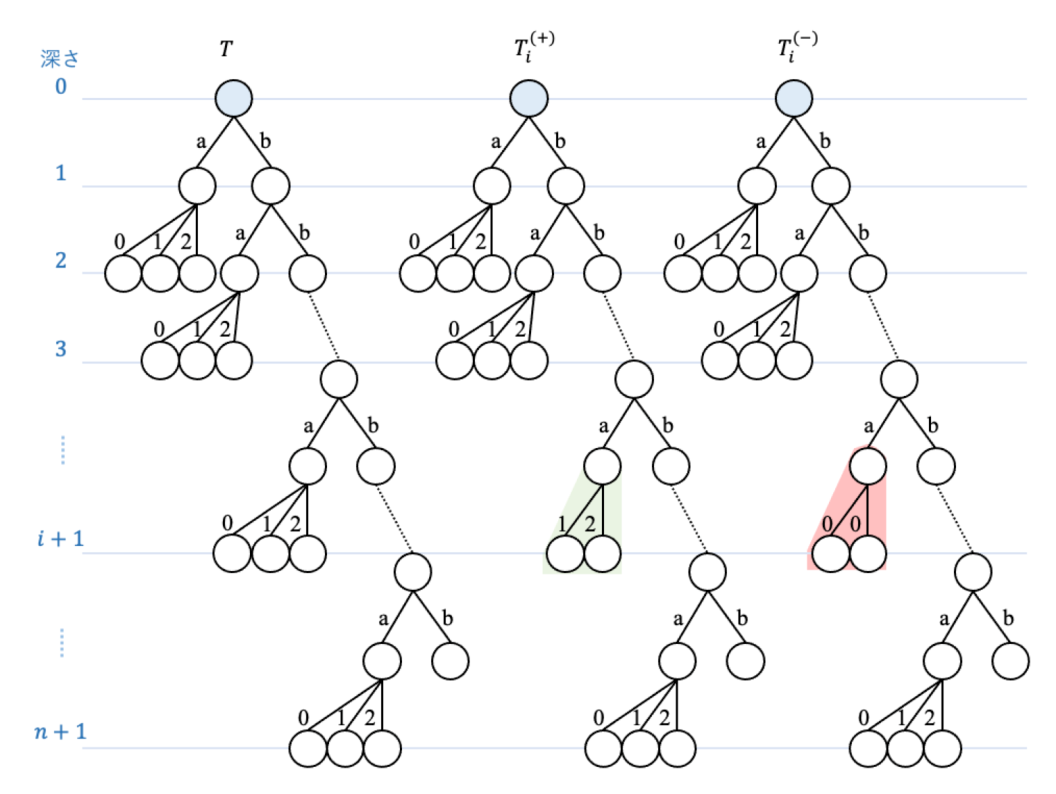
\includegraphics[scale=0.5]{fig/sample-tree.eps}
  \caption{正例と負例の元となる無順序木$T$と正例の無順序木$T_{i}^{(+)}$,負例の無順序木$T_{i}^{(-)}$ $(1\leq i\leq n)$}\label{fig:sample-tree}
\end{figure}

% 図3.2
\begin{figure}[tb]
  \centering
  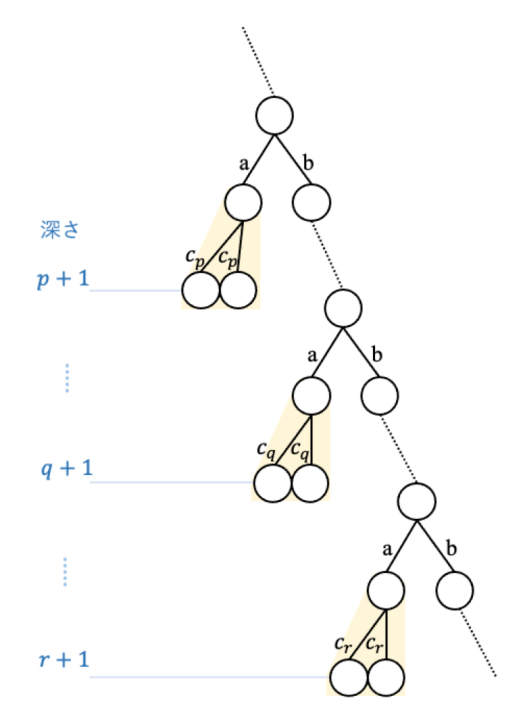
\includegraphics[scale=0.5]{fig/clause-tree.eps}
  \caption{論理変数$x_p,x_q,x_r$ $(1\leq p < q < r \leq n)$のリテラルを含む節$C_k$ $(1\leq k\leq m)$に対する$T$ (図\ref{fig:sample-tree})の変更箇所}\label{fig:clause-tree}
\end{figure}

% 図3.3
\begin{figure*}[tb]
  \centering
  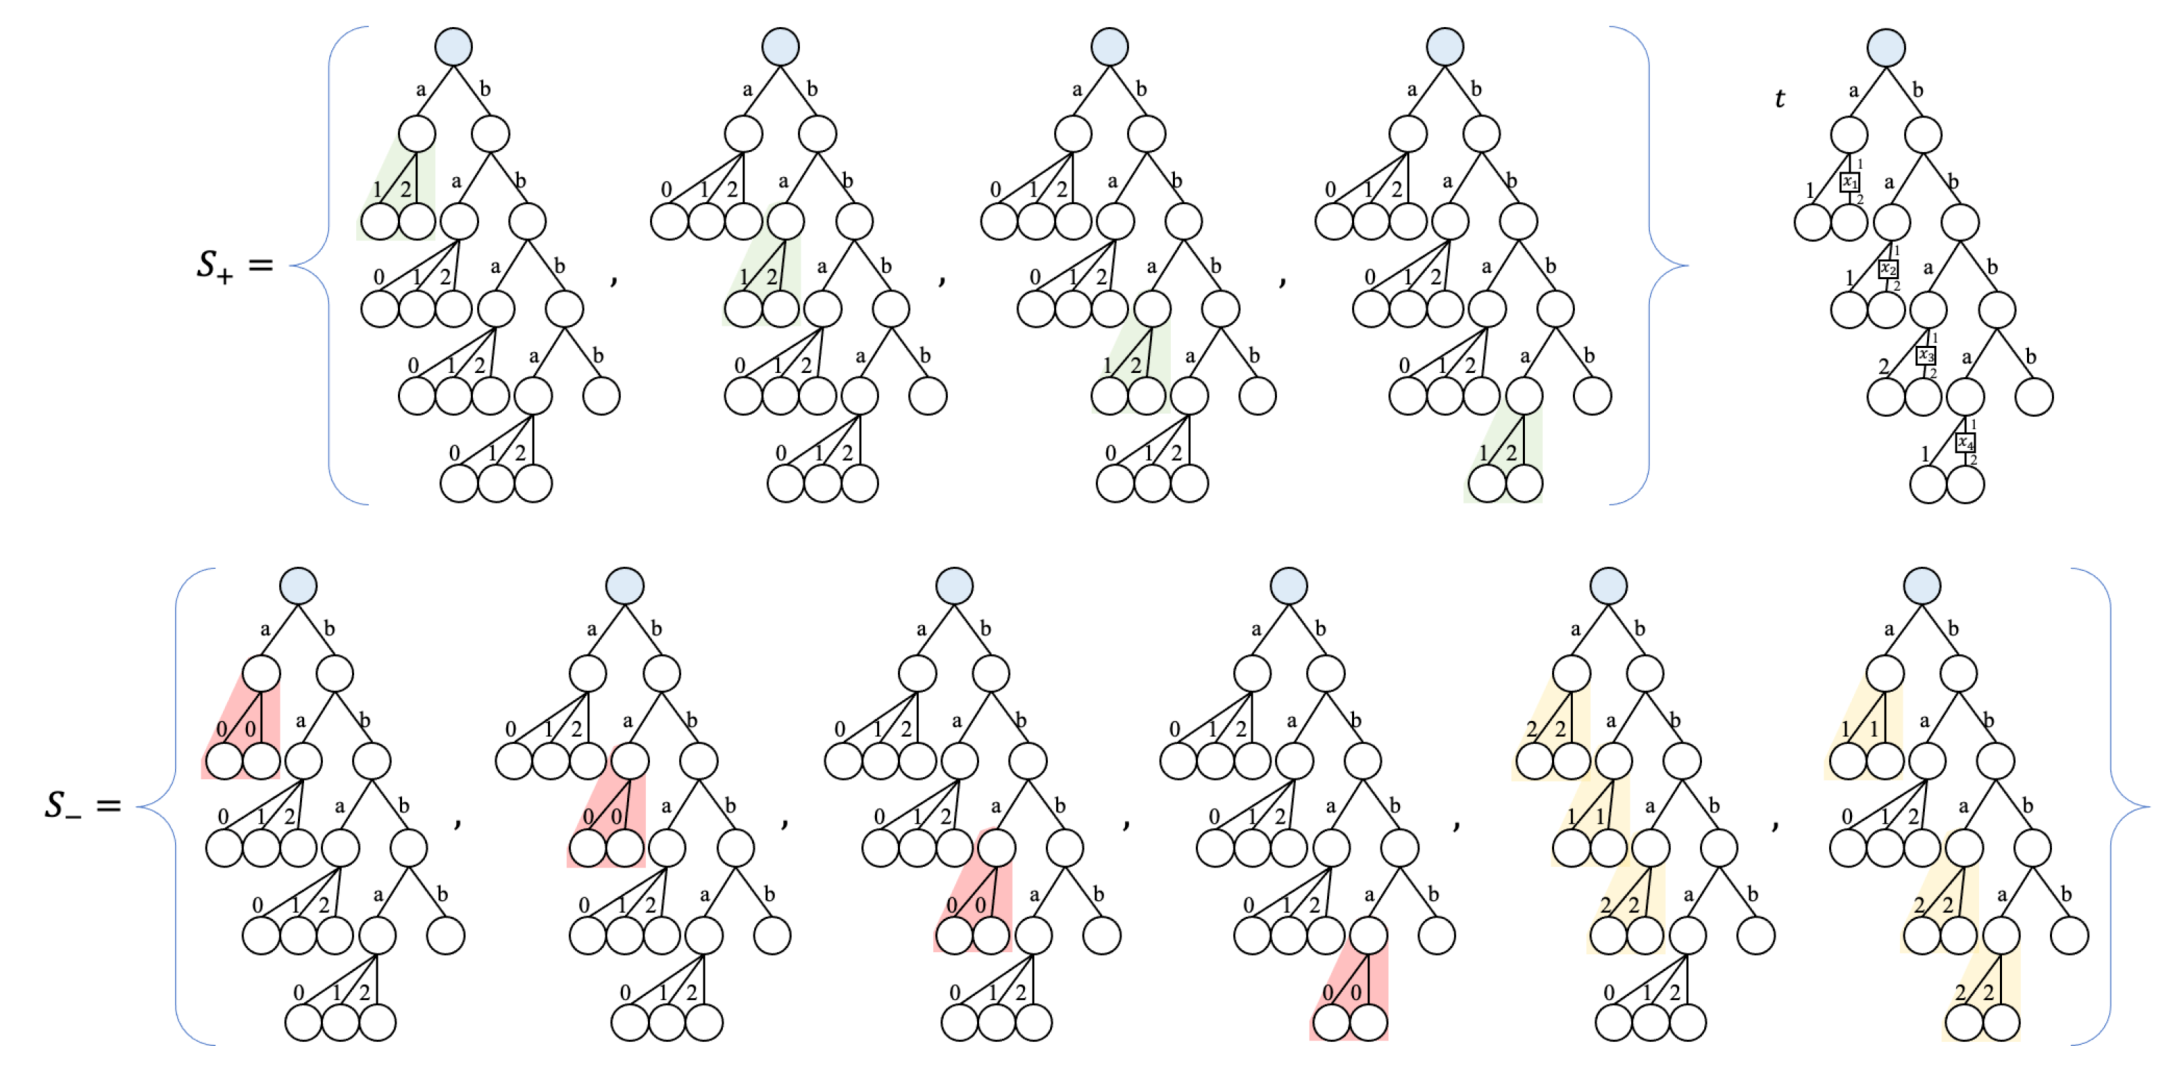
\includegraphics[scale=0.42]{fig/example_npc.eps}
  \caption{多項式時間帰着の例: 3-CNF$F=(x_{1}\vee \bar{x_{2}}\vee x_{3})\wedge(\bar{x_{1}}\vee x_{3}\vee x_{4})$に対する$S_{+}$と$S_{-}$及び,$S_+\subseteq L(t)$かつ$S_-\cap L(t)=\emptyset$を満たす線形無順序木パターン$t\in {\cal LUTP}_{\Sigma,\Lambda,X}$}\label{fig:example_npc}
\end{figure*}

\noindent
\textbf{主張 1.}
3-CNF $F$から$S_{+}, S_{-}$への変換は多項式時間で計算可能である.
\smallskip

\noindent
(主張1の証明)
$F$に現れる論理変数$x_{1},\ldots,x_{n}$から,$T_{1}^{(+)},\ldots,T_{n}^{(+)}$及び$T_{1}^{(-)},\ldots,T_{n}^{(-)}$を得るには,論理変数$x_{i}$に対して,$T$の深さ$i+1$の葉の位置を求めるだけなので,全ての論理変数に対して$n\times O(n) = O(n^{2})$時間で計算することができる.次に,$F$に現れる節$C_k$ $(1\leq k\leq m)$に対して,その節$C_k$が論理変数$x_p,x_q,x_r$ $(1\leq p < q < r \leq n)$のリテラルを含むとき,$T$の深さ$p+1, q+1, r+1$の葉の位置を求めるだけなので,全ての節に対して$m\times O(n) = O(mn)$時間で計算することができる.以上より,この変換は$n$と$m$に関する多項式時間で計算することができる.
(主張1の証明終わり)

\medskip

\noindent
\textbf{主張 2.}
3-CNF $F$を充足可能とする論理変数への論理値割り当てが存在するならば,線形無順序木パターン$t$で$S_{+}\subseteq L(t)$かつ$S_{-}\cap L(t)=\emptyset$となるものが存在する.
\smallskip

\noindent
(主張2の証明)
$F$を充足可能とする論理変数の論理値割り当てにおいて,$x_{i}$ ($1\leq i\leq n$)の論理値が$true$のとき,$T$の深さ$i+1$ ($1\leq i\leq n$)の同じ親を持つ葉の親への辺で辺ラベル$0$の辺を変数とし,$2$を辺ラベルとする親へ辺を持つ葉を削除する.また,$x_{i}$ ($1\leq i\leq n$)の論理値が$false$のとき,$T$の深さ$i+1$ ($1\leq i\leq n$)の同じ親を持つ葉の親への辺で辺ラベル$0$の辺を変数とし,$1$を辺ラベルとする親へ辺を持つ葉を削除する.このようにして,$T$から線形無順序木パターン$t$を構成する.こうして構成した線形無順序木パターンは,$S_{+}$と$S_{-}$の構成方法から,$S_{+}\subseteq L(t)$かつ$S_{-}\cap L(t)=\emptyset$を満たす.
(主張2の証明終わり)

\medskip

\noindent
\textbf{主張 3.}
線形無順序木パターン$t$で$S_{+}\subseteq L(t)$かつ$S_{-}\cap L(t)=\emptyset$となるものが存在すれば,3-CNF $F$を充足可能とする論理変数への論理値割り当てが存在する.
\smallskip

\noindent
(主張3の証明)
線形無順序木パターン$t$が$S_{+}\subseteq L(t)$かつ$S_{-}\cap L(t)=\emptyset$を満たすとする.
$t$の高さ,すなわち葉の深さの最大値は$n+1$でなければならない.なぜなら,$T_{n}^{(+)}\in L(t)$かつ$T_{n}^{(-)}\not\in L(t)$が満たされており,それら2つの無順序木の違いは同じ親を持つ深さ$n+1$の葉の親への辺ラベルだけだからである.
$t$の各頂点の子の数は高々$2$である.
$t$の根は$2$つの子を持つ.
一方の辺ラベルは$a$であり,他方は$b$である.
$a$の辺ラベルを持つ辺で繋がった根からの頂点は高々$2$つの子を持つ.
そのうち1つは,同じ深さで$3$つの子を持つ$T_{2}^{(+)},\ldots,T_{n}^{(+)}$が全て$L(t)$に属することから,変数で繋がった子となる.
一方,もう1つのこは$T_{1}^{(-)}\not\in L(t)$であることから,辺ラベル$1$または$2$を持つ辺で繋がった子である.
同様の議論により,深さ$i+1$ ($2\leq i\leq n$)の同じ親を持つ葉は2つであり,1つは$1$または$2$を辺ラベルとして持つ辺で親と繋がり,他方は変数で親と繋がる.
ここで,深さ$n-1$の葉でない頂点は2つあるが,そのうち1つは辺ラベル$b$を持つ辺で葉と繋がるか,または変数で葉と繋がるかのいずれかである.
この線形無順序木パターン$t$から,次のようにして論理変数$x_{1},\ldots,x_{n}$への論理値割り当てを構成する.
深さ$i+1$ ($1\leq i\leq n$)の同じ親を持つ2つの葉に繋がる変数でない葉の親への辺ラベルが$1$のときは,$x_{i}$の論理値を$true$に,辺ラベルが$2$のときは,$x_{i}$の論理値を$false$にする.この論理値割り当ては,各節$C_{k}$ ($1\leq k\leq m$)に対する無順序木$T_{n+k}^{(-)}$が$L(t)$に含まれないことから,$C_{k}$に現れるリテラルが全て$false$になることはない.
したがって,$S_{+}\subseteq L(t)$かつ$S_{-}\cap L(t)=\emptyset$となる線形無順序木パターン$t$が存在すれば,3-CNF $F$を充足する論理変数の論理値割り当てが存在する.
(主張3の証明終わり)

\medskip

\noindent
主張1,2,3より,${\cal LUTP}$-${\cal CP}$はNP完全である.
\end{proof}

%\end{document}

% O(N^2)
% 3.3
\subsection{$O(N^2)$回の所属性質問による質問学習アルゴリズム}
線形無順序木パターン$t_*\in {\cal LUTP}_{\Sigma,\Lambda,X}$の所属性質問に答えるオラクルを${\cal O}(t_*)$と書く.アルゴリズム${\cal LUTP}$-${\cal QUERY}_{{\cal O}(t_{\ast})}^{Square}$ (アルゴリズム\ref{alg:lutp-query-square})は,Amoth\cite{amoth-ml2001}により提案されたアルゴリズムを応用したものである.ただし,Amothのアルゴリズムは,頂点を変数とみなす無順序木構造パターンに対するアルゴリズムであるので,辺を変数とみなす本論文の線形無順序木パターンでは,もし$|\Sigma|\not=\infty$かつ$|\Lambda|\not=\infty$ならば,そのままでは正しく動作しない.

$t_*$にマッチする無順序木$T$を入力とする.このとき,${\cal LUTP}$-${\cal QUERY}_{{\cal O}(t_{\ast})}^{Square}$は,もし$|\Sigma|=\infty$または$|\Lambda|=\infty$ならば,線形無順序木パターン$t\in {\cal LUTP}_{\Sigma,\Lambda,X}$で$L(t_*)=L(t)$となる$t$を,${\cal O}(t_*)$に対して$O(N^2)$回の所属性質問を行なって正しく出力することができる.ただし,$N$は$T$の頂点数である.そのときアルゴリズム{\sc Make\_Min\_Pos\_Tree\_Sqr} (アルゴリズム\ref{alg:lutp-query-square-step1})は$t_*$にマッチする$T$を入力とした場合,その出力として,$t_*$と同じ頂点数を持ち,かつ頂点数が最小となる正例を返す.まず$T$のうち,根から最も深い頂点とその頂点に接続する辺を削除し,これを$T'$とする.次に,オラクル${\cal O}(t_*)$に$T'$を問い合わせ,${\cal O}(t_*)(T')=Yes$であれば,$T$を$T'$で更新し,${\cal O}(t_*)(T')=No$であれば,削除した頂点と辺を元に戻す.さらに,処理がいくつか進んだ後に頂点や辺の削除が成功した場合,最も深い頂点から再び順に処理を行う.この操作を再帰的に繰り返し,$T$が変化しなくなると処理を終了する.この処理により,入力された$T$が$t_*$の構造を崩すことなく正確に反映しながら特定していく.その後,頂点数最小となった無順序木$T'$を入力とするとき,もし$|\Sigma|=\infty$または$|\Lambda|=\infty$ならば,アルゴリズム\ref{alg:lutp-query-square-step2} {\sc Variable\_Specify\_Sqr}は$t_*$と同型な$t$を出力する.

具体的には,正例の子の数を$c$とするとき,$T$に現れない頂点ラベルまたは辺ラベルを貼り付けた$c+1$個の辺と頂点(熊手型)を葉に接続し,${\cal O}(t_*)(T')=Yes$であればその葉を端点とする辺を変数に置き換え,${\cal O}(t_*)(T')=No$であれば変数に置き換えず,辺のままとする.このように熊手型を代入することにより変数か否かを決定する.しかし,もし$|\Sigma|\not=\infty$かつ$|\Lambda|\not=\infty$ならば,後述する図\ref{fig:counter_leaf_to_rake}のように変数を同定できないことがある.

% アルゴリズム1
\begin{algorithm}[tb]
\caption{{\sc Make\_Min\_Pos\_Tree\_Sqr};} \label{alg:lutp-query-square-step1}
\begin{algorithmic}[1]
  \Require{$t_{\ast}\in {\cal LUTP}$の正例$T\in L(t_{\ast})$, $t_{\ast}\in {\cal LUTP}$に対する所属性質問に答えるオラクル${\cal O}(t_{\ast})$;}
  \Ensure{$T\in L(t_{\ast})$;}
  \Function{Make\_Min\_Pos\_Tree\_Sqr}{$T$};
    \State $L\coloneqq T$の葉の集合;
    \While{$L\not= \emptyset$}
      \State $T'\coloneqq T$;
      \State $\ell$を$L$の葉の1つとする;
      \State $V'$から$\ell$,$E'$から$(p(\ell),\ell)$を削除,ただし$V'$と$E'$は$T'$の頂点集合と辺集合である;
      \If{${\cal O}(t_{\ast})(T')="Yes"$}
        \State $T\coloneqq T'$;
        \State $L\coloneqq T$の葉の集合;
      \Else
        \State $L$から$\ell$を削除;
      \EndIf
    \EndWhile
    \State \Return $T$;
  \EndFunction
\end{algorithmic}
\end{algorithm}

% アルゴリズム2
\begin{algorithm}[tb]
\caption{{\sc Variable\_Specify\_Sqr};} \label{alg:lutp-query-square-step2}
\begin{algorithmic}[1]
  \Require{最小正例$T\in L(t_{\ast})$, $t_{\ast}\in {\cal LUTP}$に対する所属性質問に答えるオラクル${\cal O}(t_{\ast})$;}
  \Ensure{$t\in {\cal LUTP}$;}
  \Function{Variable\_Specify\_Sqr}{$T$}
    \State $L\coloneqq T$の葉の集合; \,$c\coloneqq \max(\deg(T))$;
    \State$t\coloneqq T$;
    \For{$\ell\in L$}
      \State $T'\coloneqq T$の$\ell$に$c+1$個の子を接続;
      \If{${\cal O}(t_{\ast})(T')="Yes"$}
        \State $T\coloneqq T'$;
        \State $T'$の$(p(\ell),\ell)$に対応する$t$の辺ラベルを変数ラベルに更新;
      \EndIf
    \EndFor
    \State \Return $t$;
  \EndFunction
\end{algorithmic}
\end{algorithm}

% アルゴリズム3
\begin{algorithm}[tb]
\caption{${\cal LUTP}$-${\cal QUERY}_{{\cal O}(t_{\ast})}^{Square}$} \label{alg:lutp-query-square}
\begin{algorithmic}[1]
  \Require{$t_{\ast}\in {\cal LUTP}$の正例$T\in L(t_{\ast})$, $t_{\ast}\in {\cal LUTP}$に対する所属性質問に答えるオラクル${\cal O}(t_{\ast})$;}
  \Ensure{$t\in {\cal LUTP}$;}
  \State $T\coloneqq $ \Call{Make\_Min\_Tree\_Sqr}{$T$};
  \State $t\coloneqq $ \Call{Variable\_Specify\_Sqr}{$T$};
\end{algorithmic}
\end{algorithm}

% O(N)
% 3.4
\subsection{$O(N)$回の所属性質問による質問学習アルゴリズム}
本章では,1つの正例を入力とするアルゴリズム${\cal LUTP}$-${\cal QUERY}_{{\cal O}(t_{\ast})}^{Linear}$が正例のサイズの線形回数の所属性質問を用いて目標とする線形無順序木パターンを同定できることを示す.一般に次のように記号を定める.無順序木$T$と無順序木パターン$t$に対して,$\Theta_t(T)= \{\theta \mid t\theta\equiv T\}$とする.また,$T$と$t$の深さ$d$の葉の集合をそれぞれ$V_d(T)$と$V_d(t)$とする.$T$の高さを$h_T$とする.

学習対象である無順序木パターンを$t_{\ast}$とし, 無順序木$T\in L(t_{\ast})$を最初に与えられる正例とする.$\Theta_{t_{\ast}}(T)\neq\emptyset$である.$T$の葉を$v$とする.$v$から根に至る道を$P_v$とするとき,$P_v$上の頂点で,子の数2以上の頂点の最大深さを$\delta_v$とする.$P$上に子の数2以上の頂点がなければ$\delta_v=0$と定める.$t_{\ast}$の変数集合を$X(t_{\ast})$とする.$x\in X(t_{\ast})$に対して,$x$の子頂点の深さを$d_x$で表す.$X_j(t_{\ast})=\{x\in X(t_{\ast}\mid j=d_x)\}$とする.$t_{\ast}$への代入$\theta=\{x\coloneqq [T_x,\sigma_x]\mid x\in X(t_{\ast})\}$が$t_{\ast}\theta \equiv T$となるとき,$\theta$によって$x$に束縛される$T$の部分木$T_x$の葉$x$と$\sigma_v$のペアの全体を$\lambda_{\theta}(x)=\{v\mid v$は$\theta$における$T_x$の葉$\}$とし,$\lambda_{(\theta,k)}(x)=\{v\mid v\in \lambda_{\theta}(x)\land \lambda_v=k\}$とする.

% アルゴリズム4
\begin{algorithm}[tb]
\caption{{\sc Variable\_Number\_Specify\_Ln};} \label{alg:lutp-query-linear-step1}
\begin{algorithmic}[1]
  \Require{$t_{\ast}\in {\cal LUTP}$の正例$T\in L(t_{\ast})$, $t_{\ast}\in {\cal LUTP}$に対する所属性質問に答えるオラクル${\cal O}(t_{\ast})$;}
  \Ensure{$T\in L(t_{\ast})$;}
  \Function{Variable\_Number\_Specify\_Ln}{$T$}
    \State $h\coloneqq T$の高さ;
    \For{$d\in [1,2,\ldots,h]~(h\geq 1)$}
      \State $L_d\coloneqq T$の深さ$d$の葉の集合;
    \EndFor
    \For{$d\in [h,h-1,\ldots,1]~(h\geq 1)$}
      \For{$\ell_d\in L_d$}
        \State $T'\coloneqq T$の$\ell_d$に$P_{h-d+1}$となるように接続;
        \If{${\cal O}(t_{\ast})(T')="Yes"$}
          \State $T\coloneqq T'$;
        \EndIf
      \EndFor
      \For{$v\in L_{d-1}$}
        \State $C := \{c_i\mid T[c_i]\equiv P_{h-d+2}(1\leq i\leq n)\}$,ただし$c_1,\ldots,c_n(n\geq 2)$は$v$の子;
        \For{$c\in C$}
          \If{$|C|>1$}
            \State $C$から$c$を削除; % $c$ \textit{from} $C$
            \State $T$から$T[c],c,(p(c),c)$を削除;
            \If{${\cal O}(t_{\ast})(T')="Yes"$}
              \State $T\coloneqq T'$;
            \EndIf
          \EndIf
        \EndFor
      \EndFor
    \EndFor
    \State \Return $T$;
  \EndFunction
  %\State 長さ$k$のチェーン(長さ$k$の道だけからなる木,$k\geq 1$)に対して,次数1の頂点を根と定めた無順序木を$P_k$で表す.
  %\State 頂点$v$の親頂点を$p(v)$で表す
  %\State $T$の頂点$v$を根とする$T$の部分無順序木を$T[v]$と記述する
  %\State $h \gets \max(depth(T))$
\end{algorithmic}
\end{algorithm}

% 補題1
\begin{lemma}\label{lemma3.1}
  アルゴリズム{\sc Variable\_Number\_Specify\_Ln} (アルゴリズム\ref{alg:lutp-query-linear-step1})の入力を$T\in L(t_{\ast})$とする.このとき関数\Call{Variable\_Number\_Specify\_Ln}{$T$}は深さ$h+1$の葉の数が$t_{\ast}$の変数の数と等しい$t_{\ast}$の正例を出力する.
  深さ$d$に対する分岐を最小にする処理終了後の$T$を$T_d$とする.任意の$\theta\in\Theta_{(t_{\ast})}(T_d)$に現れる変数$x\in X_j(t_{\ast})$に対して,$j<d$のとき,任意の$k\geq d$に対して$\abs{\lambda_{(\theta,k)}(x)}=0$,$j\geq d$のとき,$\abs{\lambda_{\theta}(x)}=1$である.
\end{lemma}

% 証明
\begin{proof}
  深さ$d$に対する高さを揃える処理終了直後の正例を$T'_d$,分岐を最小にする処理終了直後の正例を$T_d$とする.$t_{\ast}$の高さは$h_T$以下であるので,もし$t_{\ast}$の正例に深さ$h_T+1$の頂点があれば,それは$t_{\ast}$の変数に束縛される無順序木の頂点である.\\

  $d=h_T$のとき:
  \begin{enumerate}
  \item[1] $\exists\theta\in \Theta_{t_{\ast}} (T)\forall v\in V_{h_T}(T)[\tilde{v}\in V_{h_T+1}(T_{h_T})\Leftrightarrow\exists x\in X(t_{\ast})[v\in\Delta_\theta(x)]],$
  \item[2] $\forall\theta\in\Theta_{t_{\ast}}(T_{h_T})\forall\tilde{v}\in V_{h_T+1}(T_{h_T})[\exists x\in X(t_{\ast})[\Delta_\theta(x)=\{\tilde{v}\}]\lor\forall x\in X(t_{\ast})[\tilde{v}\notin\Delta_{\theta,h_t-1}(x)]]$
  \end{enumerate}
  が成り立つ.これより,$d=h_T$のとき主張が示される.\\

  $1\leq d\leq h_T$のとき:
  \begin{enumerate}
    \item[1] $\exists\theta\in\Theta_{t_{\ast}}(T_{d+1})\forall v\in \bigcup_{k=d}^{h_T}V_k(T_{d+1})[\tilde{v}\in V_{h_T+1}(T_d)\Leftrightarrow\exists x\in X(t_{\ast})[v\in\Delta_\theta(x)]]$
  \end{enumerate}
  が成り立つ.なぜなら,$t_{\ast}$において深さ$d$の葉$u$が変数の子でないとき,任意の$\theta\in\Theta_{t_{\ast}}(T_d)$に対して,$T_d$の$u$に対応する頂点$v$は$T_d$の変数に束縛される葉ではない.したがって,$\tilde{v}\notin V_{h_t+1}(T_d)$である.
  
  深さ$d-1$以上において主張が正しいと仮定する.
  \begin{enumerate}
    \item[2] $\forall\theta\in\Theta_{t_{\ast}}(T_d)\forall\tilde{v}\in V_{h_T+1}(T_d)[\exists x \in X(t_{\ast})[\Delta_\theta(x)=\{\tilde{v}\}]\lor\forall x \in X(t_{\ast})\forall j\geq d-1[\tilde{v}\notin\Delta_{\theta,j}(x)]]$
  \end{enumerate}
  深さ$d$において,次の式が成り立つ.したがって,帰納的に主張が示される.
\end{proof}


% アルゴリズム5
\begin{algorithm}[tb]
\caption{{\sc Make\_Min\_Pos\_Tree\_Ln};} \label{alg:lutp-query-linear-step2}
\begin{algorithmic}[1]
  \Require{分岐数最小正例$T\in L(t_{\ast})$, $t_{\ast}\in {\cal LUTP}$に対する所属性質問に答えるオラクル${\cal O}(t_{\ast})$;}
  \Ensure{$T\in L(t_{\ast})$;}
  \Function{Make\_Min\_Pos\_Tree\_Ln}{$T$}
    \For{$d\in [1,2,\ldots,h]~(h\geq 1)$}
      \State $V_d\coloneqq L$の深さ$d$の部分集合;
      \For{$v\in V_d$}
        \If{$T[v]\equiv P_{h-d+1}$}
          \State $T$から$T[v]$を削除,ただし,$v$と$(p(v),v)$は削除しない;
          \If{$d\neq \max(depth(T))-1$}
            \If{${\cal O}(t_{\ast})(T')="Yes"$}
              \State $T\coloneqq T'$;
            \EndIf
          \Else
            \State $T\coloneqq T'$;
          \EndIf
        \EndIf
      \EndFor
    \EndFor
    \State \Return $T$;
  \EndFunction
\end{algorithmic}
\end{algorithm}


% 補題2
\begin{lemma}\label{lemma3.2}
  関数\Call{Variable\_Number\_Specify\_Ln}{$T$}の出力を$T\in L(t_{\ast})$とする.このときアルゴリズム\ref{alg:lutp-query-linear-step2} \Call{Make\_Min\_Pos\_Tree\_Ln}{$T$}は$t_{\ast}$の変数を辺に置き換えて得られる$t_{\ast}$の最小正例を出力する.
  深さ$d$に対する関数\Call{Make\_Min\_Pos\_Tree\_Ln}{$T$}終了後の$T$を$T_d$とする.任意の$\theta\in\Theta_{t_{\ast}}(T_d)$に対して,$\theta$に現れる変数$x\in X_j(t_{\ast})(1\geq j\geq d)$に束縛される無順序木はただ1つの辺から成る.
\end{lemma}


% 証明
\begin{proof}
  関数\Call{Variable\_Number\_Specify\_Ln}{$T$}終了後の$T$を$T_0$とする.任意の$\theta\in\Theta_{t_{\ast}}(T_{d-1})(d\geq1)$に対して,変数$x\in X_d(t_{\ast})$には,$P_{h_T-d+2}$が束縛されている.深さ$d$の処理後,$\abs{V_d(T_d)}=\abs{V_d(t_{\ast})}$となる.
  したがって,主張が示される.
\end{proof}


% アルゴリズム6
\begin{algorithm}[tb]
\caption{{\sc Variable\_Specify\_Ln};} \label{alg:lutp-query-linear-step3}
\begin{algorithmic}[1]
  \Require{最小正例$T\in L(t_{\ast})$, $t_{\ast}\in {\cal LUTP}$に対する所属性質問に答えるオラクル${\cal O}(t_{\ast})$;}
  \Ensure{$t\in {\cal LUTP}$;}
  \Function{Variable\_Specify\_Ln}{$T$}
    \State $h\coloneqq \max(depth(T))$
    \State $T=(V,E)$を左深さ優先木に更新;
    \For{$v\in V$}
      \State $c_1,\ldots,c_n(c\geq 2)\coloneqq v$の子,ただし,$T[c_1],T[c_2],\ldots,T[c_n]$は降順である;
      \For{$c\in [c_1,c_2,\ldots,c_n]$}
        \If{$T[c]$が長さ0以上のチェーン}
          \State $l\coloneqq T[c]$の葉;
          \State $T'\coloneqq T[c]$に$P_{h-d+1}$となるように接続;
          \If{${\cal O}(t_{\ast})(T')="Yes"$}
            \State $T\coloneqq T'$;
            \State $(p(v),v)$を変数$[p(v),v]$に更新;
          \EndIf
        \EndIf
      \EndFor
    \EndFor
    \State \Return $t$;
  \EndFunction
\end{algorithmic}
\end{algorithm}


関数\Call{Make\_Min\_Pos\_Tree\_Ln}{$T$}の出力$T$の頂点を左深さ優先順に処理する.以下では任意の$ v\in V(T)$の子$c_1,c_2,\ldots,c_m(m\geq2)$を根とする部分木$T[c_1],T[c_2],\ldots,T[c_m]$は左深さ優先順であるとする.頂点$v\in V(T)$の深さを$d_v$で表す.\par
$T$の子の数2以上の子孫を持つ頂点を左深さ優先順に帰りがけ順で並べた頂点列を$v_1,\ldots,v_{n'}(n'\geq1)$とする.$v_1,\ldots,v_{n'}$は処理が実行される頂点で,この頂点順に処理が終了する.すなわち,$v_{n'}$は$T$の根である.(本論文では,頂点$v$は$v$自身の子孫であるとする.)
また,アルゴリズム\ref{alg:lutp-query-linear-step3} {\sc Variable\_Specify\_Ln}内において,深さ$d_{v_i}$にある頂点$v_i$を根とする部分木$T[v_i]$の変数を特定する処理をFind\_Variable($T[v_i],d_{v_i}$)と記す.


% 補題3
\begin{lemma}\label{lemma3.3}
  関数\Call{Make\_Min\_Pos\_Tree\_Ln}{$T$}の出力を$T\in L(t_{\ast})$とする.このとき関数\Call{Variable\_Specify\_Ln}{$T$}は$t_{\ast}$を出力する.
  任意の$k(1\leq k\leq n')$に対して,$i(1\leq i\leq k)$に対するFind\_Variable($T[v_i],d_{v_i}$)が$t_{\ast}$の変数に対応する$T[v_i]$の辺を正しく特定しているとき,Find\_Variable($T[v_k],d_{v_k}$)は$t_{\ast}$の変数に対応する$T[v_k]$の辺を正しく特定する.
\end{lemma}


% 証明
\begin{proof}
  $v_{k-1},v_k(1<k\leq n')$の関係について場合分けにより証明する.
  \begin{enumerate}
    \item[(i)] $v_1$について:\\
                $T[v_1]$は左深さ優先順である.変数位置の特定には深さが$h_T+1$になるよう道を付加するので,$T[v_1]$が左深さ優先で最左であることが常に保証される.故にFind\_Variable($T[v_1],d_{v_1}$)は$t_{\ast}$の変数に対応する$T[v_1]$の辺を正しく特定する.
    \item[(ii)] $v_k$が$v_{k-1}$の親であるとき:\\
                $v_k$の子に対するFind\_Variableは全て正しく終了している.よって,$t_{\ast}$の変数に対応する$T[v_k]$の辺は既に正しく特定されている.
    \item[(iii)] $v_k$が$v_{k-1}$の兄弟であるとき:\\
                $v$を$v_k$の任意の真の先祖,$v$の子を$c_1,\ldots,c_m(m\geq2)$とし,$T[c_j](1\leq j\leq m)$が$v_k$を含むとする.$c_1,\ldots,c_m$に対応する$t_{\ast}$の頂点を$c'_1,\ldots,c'_m(m\geq2)$とする.Find\_Variable($T[c_j],d_{c_j}$)が実行されているとき,任意の$\beta(j<\beta\leq m)$に対して,$T[c_\beta]$が$T[c_j]$と異なる深さ列を持つならば,$t_{\ast}[c'_j]$が$T[c_\beta]$にマッチすることはない.\\
                なぜなら,無順序木パターンがその深さ列より小さい無順序木にマッチすることはないからである.$T_[c_\beta]$が$T[c_j]$と同じ深さ列を持つならば,$T[c_j]$の処理における$t_{\ast}[c'_j]$の変数位置は,$T[c_\beta]$に対応する$t_\ast [c'_j]$の変数位置より深さ優先で特定される.\\
                一方,任意の$\alpha(1\leq\alpha<j)$では,既にFind\_Variable($T[c_\alpha],d_{c_\alpha}$)の実行は終了しているので,$T[c_\alpha]$における$t_\ast [c'_\alpha]$に対応する変数の位置は特定されている.もし,Find\_Variable($T[c_j],d_{c_j}$)を実行中の$T[c_j]$に$\gamma '(\gamma '<j)$が存在して$t_\ast[c'_{\gamma '}]$がマッチすれば,$\gamma(\gamma<j)$が存在して$t_\ast [c'_j]$はすでに変数位置が特定されている$T[c_\gamma]$にマッチする.\\
                このとき$T[c_\gamma]$の深さ列は$T[c_j]$のそれ以上なので,Find\_Variable($T[c_j],d_{c_j}$)の実行中に変数判定を行う辺は,$T[c_\gamma]$において既に変数であると判定されている.したがってFind\_Variable($T[c_j],d_{c_j}$)は$T[c_j]$の変数位置を正確に特定する.
                以上より,Find\_Variable($T[c_j],d_{c_j}$)で実行されるFind\_Variable($T[v_k],d_{v_k}$)も$t_\ast$の変数に対応する$T[v_k]$の辺を正しく特定する.
    \item[(iv)] $v_k$が$v_{k-1}$の兄弟の子孫であるとき:\\
                $v_k$と$v_{k-1}$の共通の先祖$v$について(iii)と同様に示される.
  \end{enumerate}
\end{proof}

% アルゴリズム7
\begin{algorithm}[tb]
\caption{${\cal LUTP}$-${\cal QUERY}_{{\cal O}(t_{\ast})}^{Linear}$} \label{alg:lutp-query-linear}
\begin{algorithmic}[1]
  \Require{$t_{\ast}\in {\cal LUTP}$の正例$T\in L(t_{\ast})$, $t_{\ast}\in {\cal LUTP}$に対する所属性質問に答えるオラクル${\cal O}(t_{\ast})$;}
  \Ensure{$t\in {\cal LUTP}$;}
  \State $T\coloneqq $ \Call{Variable\_Number\_Specify\_Ln}{$T$};
  \State $T\coloneqq $ \Call{Make\_Min\_Tree\_Ln}{$T$};
  \State $t\coloneqq $ \Call{Variable\_Specify\_Ln}{$T$};
\end{algorithmic}
\end{algorithm}

% 定理2
\begin{theorem}\label{theorem3}
  無順序木パターン$t_{\ast}\in {\cal LUTP}_{\Sigma, \Lambda, X}$に対する所属性質問に答えるオラクル${\cal O}(t_{\ast})$を仮定する.
  頂点数$N(N\geq 5)$の正例$T\in L(t_{\ast})$が与えられたとき,${\cal O}(t_{\ast})$への高々$4N$回の所属性質問を行うことで,$t_\ast$の表現,すなわち$L(t_\ast)=L(t)$となる線形無順序木パターン$t\in{\cal LUTP}$を同定可能である.
  %(1)線形無順序木パターン$t_{\ast}\in{\cal LUTP}_{\Sigma,\Lambda,X}$に対する所属性質問に答えるオラクル${\cal O}(t_{\ast})$を仮定する.頂点数$N$の正例$T\in L(t_{\ast})$が与えられたとき,${\cal O}(t_{\ast})$への$O(N)$回の所属性質問を行うことで,$L(t_{\ast})=L(t)$となる無順序木パターン$t\in{\cal LUTP}_{\Sigma,\Lambda,X}$を同定可能である.
  %(2)無順序木パターン$t_{\ast}\in {\cal LUTP}_{\Sigma, \Lambda, X}$に対する所属性質問に答えるオラクル$\mathcal{O}(t_{\ast})$を仮定する.頂点数$N(N\geq 5)$の正例$T\in L(t_{\ast})$が与えられたとき,$\mathcal{O}(t_{\ast})$への高々$4N$回の所属性質問により,$t_{\ast}$の表現,すなわち$t=(V_t, E_t, H_t)$を同定可能である.
\end{theorem}

\begin{proof}
  正例の無順序木の頂点数を$N$とするとき,アルゴリズム\ref{alg:lutp-query-linear-step1}の6--12行において,深さごとにチェーン型の無順序木を代入して,オラクルに問い合わせを行う回数は高々$N$回,15--23行において,深さごとに分岐を削除して,オラクルに問い合わせを行う回数は高々$N$回である.アルゴリズム\ref{alg:lutp-query-linear-step2}において,根に近い道の長いチェーン型の無順序木を順に短くして,オラクルに問い合わせを行う回数は高々$N$回である.アルゴリズム\ref{alg:lutp-query-linear-step3}において,葉にチェーン型の無順序木を代入して,高々$N$回オラクルへの所属性質問で変数か否かを判定する.したがって,合計で${\cal O}(t_{\ast})$への高々$4N$回の所属性質問を行うことで,$t_\ast$の表現,すなわち$L(t_\ast)=L(t)$となる線形無順序木パターン$t\in{\cal LUTP}$を同定可能である.アルゴリズムの正当性は,補題\ref{lemma3.1}, \ref{lemma3.2}, \ref{lemma3.3}より証明される.以上より,本定理が得られる.
\end{proof}

% 3.5
\subsection{質問戦略に関する考察}
これより,アルゴリズム${\cal LUTP}$-${\cal QUERY}_{{\cal O}(t_{\ast})}^{Linear}$(アルゴリズム\ref{alg:lutp-query-linear})を設計するにあたり,発生した問題点と改善点を述べる.

まず,はじめのアプローチとして,最小正例の発見と変数の特定を同時に行うために正例集合に現れる子の頂点数$c$に1を加えた$c+1$個の葉を持つ構造を生成し,これを熊手型と呼ばれる無順序木として葉に代入する手法(以降,熊手戦略と呼ぶ)を採用した.具体的には,アルゴリズム${\cal LUTP}$-${\cal QUERY}_{{\cal O}(t_{\ast})}^{Square}$では関数\Call{Make\_Min\_Tree\_Sqr}{$T$}において辺を削除することで最小正例を発見し,関数\Call{Variable\_Specify\_Sqr}{$T$}において熊手戦略を用いることによって変数を特定していた.そこで,この2つのステップを同時に行うことで既存手法より質問回数の少ないアルゴリズムを開発し,目標の線形無順序木パターンを発見することを試みた.しかし,図\ref{fig:counter_leaf_to_rake}に示す例によりパターンを発見することが困難であることが確認できた.具体的には,葉に直接,熊手型を接続するため,無順序木の性質上,接続された熊手型の無順序木が,同様の構造を持つ他の部分木にも適用されてしまう可能性がある.その結果,線形無順序木パターンから見ると本来は代入すべきでない箇所にも誤って熊手型の無順序木が代入されてしまい,対象とする構造が正確に反映されない問題が生じる.このように,構造を横方向に広げて処理を進める熊手戦略は,無順序木のように見かけ上一意に定まらない構造に対しては不適切であることが確認できた.

熊手戦略では,無順序木の性質に起因する誤代入が生じやすく,正例の構造を正確に反映することが困難である.そこで,正例となる無順序木の高さを$H_T$とした場合,葉に対して$H_T$よりも1長い位置まで道を付加する方法を取る.この手法は,構造を縦方向に広げながら処理を進めることからチェーン戦略と呼ぶ.チェーン戦略の特徴は,縦方向に構造を拡張することで分岐を持たない無順序木を代入する点にある.このアプローチにより,無順序木の特性に依存した代入の曖昧性が解消され,他の部分木に誤って適用されることがない.結果として,正例の構造を正確に反映しながら,正確な処理が可能となる.チェーン戦略は,無順序木における構造の一意性を保証し,パターンの特定において重要な役割を果たす.

% 図3.4
\begin{figure*}[tb]
  \centering
  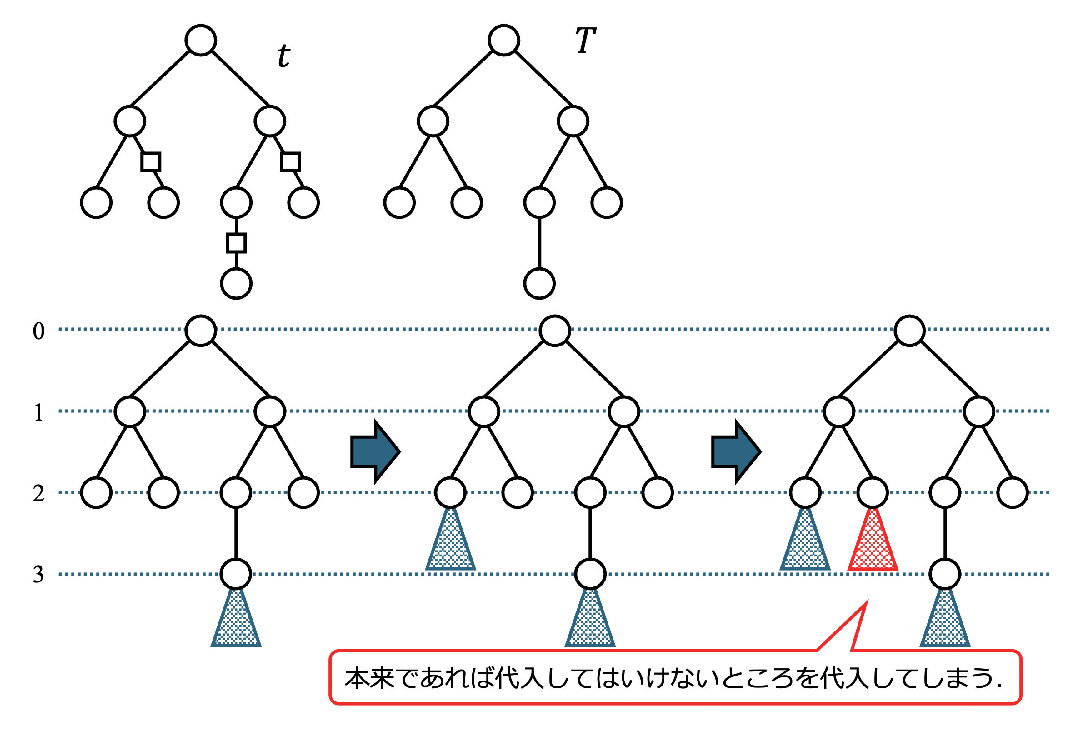
\includegraphics[scale=0.6]{fig/fig-counter_leaf_to_rake.eps}
  \caption{線形無順序木パターン$t$と正例となる無順序木$T$に対して,熊手戦略を用いて辺縮約と変数同定を同時に処理すると,本来であれば変数として扱うべきでない辺を誤って変数と位置づけてしまう問題が生じる.}\label{fig:counter_leaf_to_rake}
\end{figure*}

次に,チェーン型の無順序木を葉に代入し,高さを揃えることで目標とする線形無順序木パターンを発見できることが確認できた.一見すると関数\Call{Make\_Min\_Tree\_Sqr}{$T$}まででパターンを発見できているように見えるがそうではない.図\ref{fig:counter_step1_2}に具体例を示す.上段では,関数\Call{Variable\_Number\_Specify\_Ln}{$T$}の処理を示している.このアルゴリズムが終了した段階では,正例として与えられる無順序木の高さ$H_T$を超える位置に道を追加することで,変数の数と分岐の数が一致することを確認できる.この処理により,無順序木における変数の位置や数が適切に特定され,次の処理への準備が整う.
一方で,最小の正例を特定する関数\Call{Make\_Min\_Tree\_Ln}{$T$}(図\ref{fig:counter_step1_2}の下段)では,無順序木の持つ特性が障害となる場合がある.具体的には,削除を行う順番が影響を及ぼし,削除が完了した部分が定数として誤って解釈される可能性が生じる.このような場合,処理の進行中に本来変数とみなすべき箇所が定数とみなされることで,意図した通りの変数の位置を特定できなくなるリスクがある.そのため,最小の正例を発見する処理とは別で変数を特定する処理が必要である.

% 図3.5
\begin{figure*}[tb]
  \centering
  \includegraphics[scale=0.5]{fig/fig-counter_step1_2.eps}
  \caption{線形無順序木パターン$t$と正例となる無順序木$T$に対して,最小正例を発見するまでで処理を終了すると,熊手型の無順序木が存在する箇所と変数であるべき位置が一致しないため,パターンの発見には至らない.}\label{fig:counter_step1_2}
\end{figure*}

しかし,関数\Call{Make\_Min\_Tree\_Sqr}{$T$}終了後,無順序木を対象としているため,必ずしも見かけ上同型の最小正例を発見することができない.そこで,本研究では無順序木の構造を一意に定めるために左深さ優先木を導入した.左深さ優先木とは,無順序木における各頂点の子の順序を深さ列が最大となるように並び替えて構築される一意に定められる木構造である.この定義に基づき,まず無順序木を左深さ優先木に変換して,構造を一意化する.これにより,アルゴリズム処理における誤解釈の可能性を取り除くことで正確な処理が可能となる.さらに,左深さ優先木への変換によって得られる一意性は,変数の位置特定の処理において重要な役割を果たす.図\ref{fig:counter_ldfs_tree}では,左深さ優先木に変換した場合と変換しない場合の違いを具体的に示している.上段は,図\ref{fig:counter_step1_2}の続きから左深さ優先木に変換しない場合を示しており,この場合,変数を特定する順番が一意に定まらず,代入が正しく行われない場合がある.その結果,変数を正確に特定することができず,対象とする木構造を完全には反映できない.一方,下段では左深さ優先木に変換した場合の結果を示している.この場合,左深さ優先の基準に基づいて木構造を一意に定めている.その上で,チェーン戦略を用いることにより,変数を特定することが可能になる.具体的には,代入したチェーン型の無順序木の深さ列が左の部分木の深さ列を超えることがないため,変数の代入が正確に行われる.この手法により,元の無順序木パターンを忠実に再現することが可能になる.

% 図3.6
\begin{figure*}[tb]
  \centering
  \includegraphics[scale=0.5]{fig/fig-counter_ldfs_tree.eps}
  \caption{線形無順序木パターン$t$と正例となる無順序木$T$に対して,最小正例が得られた場合でも,無順序木である特性上,変数を特定する順番によっては元のパターンを再現できないことがある(図上).一方で,左深さ優先木に変換することで無順序木が一意に定まるため,元のパターンを正確に再現することが可能となる(図下).}\label{fig:counter_ldfs_tree}
\end{figure*}

% 3.6
\subsection{アルゴリズム${\cal LUTP}$-${\cal QUERY}_{{\cal O}(t_{\ast})}^{Linear}$の実験的解析}
人工データを用いて行なった2つの計算機実験による解析結果を報告する.本実験では${\cal LUTP}$の所属性質問を行う際のオラクルとして,Shoudaiら\cite{shoudai-ieice2018}によって提案された線形無順序項木パターンの多項式時間マッチングアルゴリズムを使用した.このアルゴリズムは,学習目標である無順序木パターン$t_\ast\in{\cal LUTP}$から照合のためのルールを作成して無順序木$T$の頂点と$t_\ast$の頂点の間の対応関係を求める.それにより$t_\ast$が$T$とマッチするか否かを判定する.

% 3.6.1
\subsubsection{最小正例から同定する際の質問回数の解析} \label{qltimes_input_min}
オラクル${\cal O}(t_\ast)$を用いた質問学習アルゴリズム${\cal LUTP}$-${\cal QUERY}_{{\cal O}(t_{\ast})}^{Linear}$の入力を$t_\ast$の変数を辺とみなした無順序木$T_{t_\ast}$として各ステップでオラクル${\cal O}(t_\ast)$に所属性質問を行う回数を求める.すなわち,アルゴリズム${\cal LUTP}$-${\cal QUERY}_{{\cal O}(t_{\ast})}^{Linear}$への入力を,学習目標である$t_\ast\in{\cal LUTP}$の頂点数最小の正例とする.ここでは,あらかじめ定められた頂点数を持つ全ての無順序木を解析対象とするために,無順序木の列挙アルゴリズム\cite{nii-nakano_uno2003,cs-nakano_uno2004}を使用して,頂点数21まで全無順序木を生成した.生成した各無順序木の葉辺を変数に置き換えることによって,全ての無順序木パターンを作成して,頂点数と所属性質問を行う回数に関する解析を行った.ただし,頂点数2から13は全ての無順序木パターンに対して解析を行なったが,頂点数14以降は計算時間が非常に大きくなるため,頂点数13の無順序木パターンの数409963個を参考に410000個の無順序木パターンをランダムに生成して解析を行った.

実験結果の折れ線グラフを図\ref{fig:qltimes_input_min}に,その数値結果を表\ref{tbl:qltimes_input_min}に示す.横軸に頂点数,縦軸に質問回数を表す.各頂点の質問回数に対して最大値を青色,最小値を緑色,平均値を橙色でプロットして折れ線グラフで表現する.いずれも定数倍で増加していることが確認できる.全ての無順序木パターンを解析した頂点数13までの結果から,頂点数を$N(N\geq5)$とするとき,質問回数の最大値が$4(N-2)$(図\ref{fig:qltimes_input_min}: 青破線),最小値が4(図\ref{fig:qltimes_input_min}: 緑破線)であることが確認できる.
実験により,質問回数が最大となる無順序木パターン$t_{max}$は,$N\geq5$の場合,葉辺が変数である長さ2のチェーンが1つと葉辺に変数を持つ長さ1のチェーンが2以上ある場合であることが確認できる(図\ref{fig:qltimes_max_min}(左)).これは根と$N-1$個の葉が接続された無順序木パターンに比べ,アルゴリズム\ref{alg:lutp-query-linear-step2}で深さ1または2のどちらが変数であるか検証する必要があるため質問回数が多くなる.$N=2,3,4$の場合の最大質問回数はそれぞれ3,6,9である.また,質問回数が最小となる無順序木パターン($N\geq3$)は図\ref{fig:qltimes_max_min}の右に示す無順序木パターン$t_{min}$である.図\ref{fig:qltimes_max_min}では$t_{min}$の頂点集合を$\{u_1,u_2,\ldots,u_n\}~(n=N,N\geq3)$としている.根$u_1$から頂点$u_{n-2}$まで分岐を持たない頂点が接続されており,$u_{n-2}$に接続する長さ1のチェーンで葉辺が変数であるものが1つ,葉辺が辺であるものが1つ持つ場合である.この無順序木パターンは,頂点数$N$のチェーンである無順序木パターンに比べ,アルゴリズム\ref{alg:lutp-query-linear-step2}でのチェーンを短くするための質問を行う必要がない.そのため,質問回数が最小となる.

% 図3.7, 表3.1
\begin{figure}[tb]
  \begin{center}
  % 図
 % \begin{minipage}[c]{0.5\hsize}
 %   \centering
    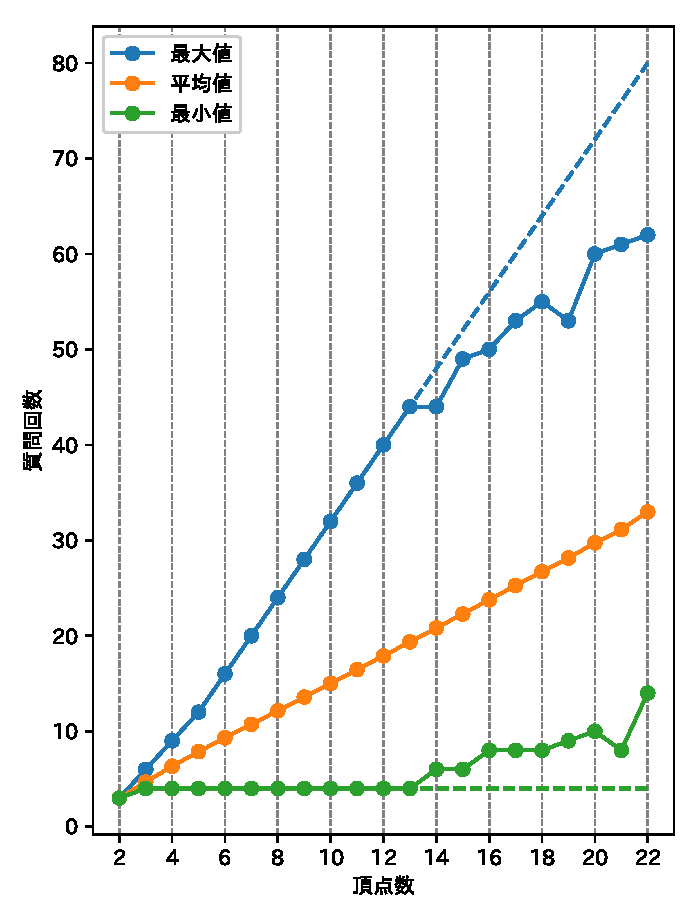
\includegraphics[scale=0.7]{fig/fig-qltimes_input_min.eps}
    \caption{入力が最小正例とするときの質問回数の推移}\label{fig:qltimes_input_min}
 % \end{minipage}
  %\hspace{0.02\hsize} % ここで隙間作成
  \vspace*{10.5pt}
  % 表
 % \begin{minipage}[c]{0.5\hsize} % 表を並べることが可能
 %   \centering
    \tblcaption{図\ref{fig:qltimes_input_min}の数値結果}\label{tbl:qltimes_input_min}
    \begin{tabular}{rrrrr} \hline
      頂点数 &  木の数 & 最大値 & 最小値 & 平均値 \\ \hline\hline
          2 &      1 &     3 &     3 &  3.00 \\
          3 &      3 &     6 &     4 &  4.67 \\
          4 &      9 &     9 &     4 &  6.33 \\
          5 &     28 &    12 &     4 &  7.86 \\
          6 &     88 &    16 &     4 &  9.31 \\
          7 &    284 &    20 &     4 & 10.73 \\
          8 &    927 &    24 &     4 & 12.15 \\
          9 &   3074 &    28 &     4 & 13.57 \\
         10 &  10300 &    32 &     4 & 15.01 \\
         11 &  34880 &    36 &     4 & 16.45 \\
         12 & 119109 &    40 &     4 & 17.90 \\
         13 & 409963 &    44 &     4 & 19.35 \\
         14 & 410000 &    44 &     6 & 20.82 \\
         15 & 410000 &    49 &     6 & 22.28 \\
         16 & 410000 &    50 &     8 & 23.77 \\
         17 & 410000 &    53 &     8 & 25.27 \\
         18 & 410000 &    55 &     8 & 26.72 \\
         19 & 410000 &    53 &     9 & 28.14 \\
         20 & 410000 &    60 &    10 & 29.73 \\
         21 & 410000 &    61 &     8 & 31.12 \\ \hline
    \end{tabular}
 % \end{minipage}
  \end{center}
\end{figure}
0
% 図3.8
\begin{figure}[tb]
  \centering
  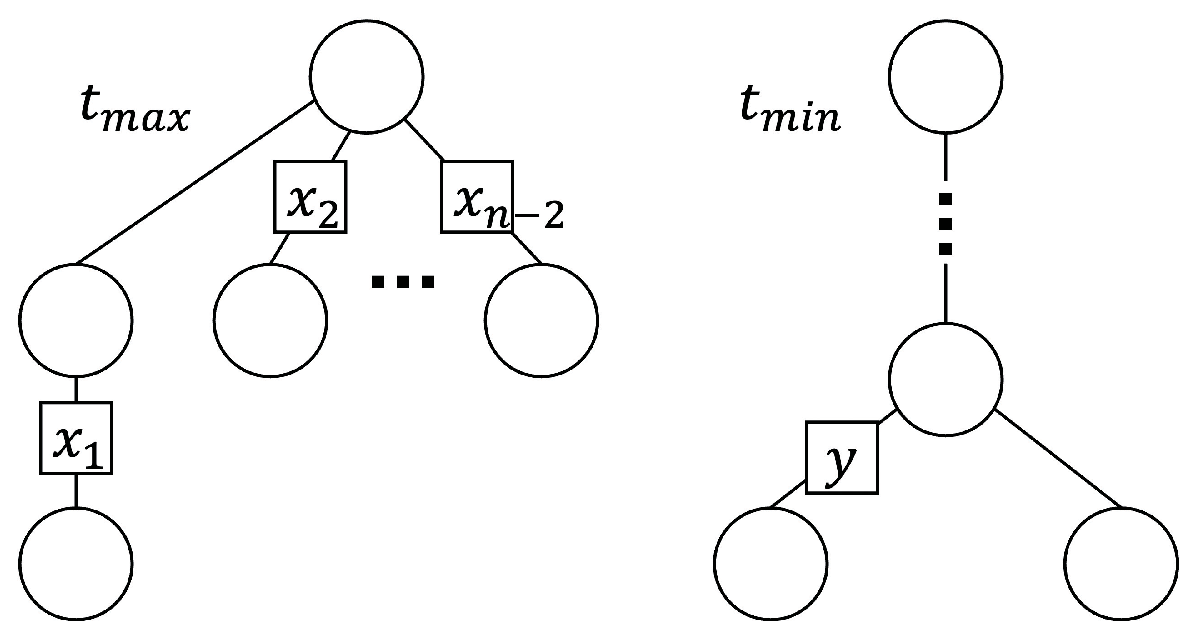
\includegraphics[scale=0.34]{fig/fig-qltimes_max_min.eps}
  \caption{頂点数が同じとき質問回数が$4(N-2)$~($N$は入力となる正例の頂点数)で最大となる無順序木パターン$t_{max}$と,4で最小となる無順序木パターン$t_{min}$}\label{fig:qltimes_max_min}
\end{figure}

% 3.6.2
\subsubsection{正例の葉の数に関する質問回数の解析}
アルゴリズム${\cal LUTP}$-${\cal QUERY}_{{\cal O}(t_{\ast})}^{Linear}$への入力の頂点数を,学習目標である$t_\ast\in{\cal LUTP}$の頂点数の1倍から2倍まで変化させて,正例の葉の数に関する質問回数の解析を行なった.\ref{qltimes_input_min}項において全ての無順序木パターンを調査することができた頂点数13を対象とし,頂点数13から成る無順序木パターン$t_\ast$に対して,正例となる頂点数26の無順序木をランダムに100個生成した.生成した正例の集合を$S_+$とする.$S_+$に属す無順序木を${\cal LUTP}$-${\cal QUERY}_{{\cal O}(t_{\ast})}^{Linear}$の入力として,アルゴリズム\ref{alg:lutp-query-linear-step1}まで行う.これをランダムに40000回繰り返した.異なる入力(無順序木)であっても学習目標である無順序木パターン$t_\ast$が同じであれば,無順序木の頂点数に関わらずアルゴリズム\ref{alg:lutp-query-linear-step2}とアルゴリズム\ref{alg:lutp-query-linear-step3}の質問回数は変わらないので,本実験はアルゴリズム\ref{alg:lutp-query-linear-step1}まで実行する.その結果を下記に解析する.

実験結果の折れ線グラフを図\ref{fig:qltimes_input_twice}に,その数値結果を表\ref{tbl:qltimes_input_twice}に示す.入力となる無順序木の頂点数を固定した場合,質問回数は無順序木の葉の数に比例して増加することが確認できる.質問回数は,無順序木の頂点数に関わらず,葉の数のみに依存する.また,アルゴリズム\ref{alg:lutp-query-linear-step1}までの質問回数は葉の数の2倍以下であることが確認できる.これは,葉にチェーン型を代入するステップと分岐を減らすステップを同じ深さで行っているからである.すなわち,定理\ref{theorem3}と同じ結果になることが確認できる.

% 図3.9, 表3.2
\begin{figure}[tb]
  \begin{center}
  % 図
  %\begin{minipage}[c]{0.5\hsize}
  %  \centering
    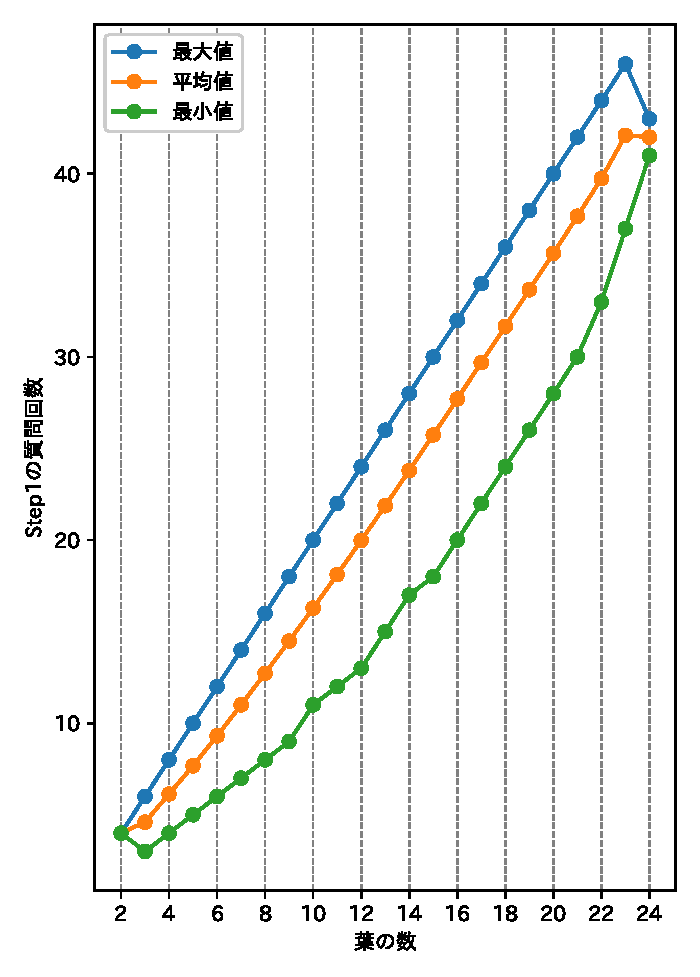
\includegraphics[scale=0.7]{fig/fig-qltimes_input_twice.eps}
    \caption{入力が最小正例とするときの質問回数の推移}\label{fig:qltimes_input_twice}
  %\end{minipage}
  %\hspace{0.02\hsize} % ここで隙間作成
  \vspace*{10.5pt}
  % 表
  %\begin{minipage}[c]{0.5\hsize} % 表を並べることが可能
  %  \centering
    \tblcaption{図\ref{fig:qltimes_input_twice}の数値結果}\label{tbl:qltimes_input_twice}
    \begin{tabular}{rrrrr} \hline
      葉の数 &   木の数 & 最大値 & 最小値  & 平均値 \\ \hline\hline
          2 &       1 &     4 &     4  &  4.00 \\
          3 &      15 &     6 &     3  &  4.60 \\
          4 &     238 &     8 &     4  &  6.13 \\
          5 &    3747 &    10 &     5  &  7.67 \\
          6 &   30859 &    12 &     6  &  9.31 \\
          7 &  168767 &    14 &     7  & 11.00 \\
          8 &  646945 &    16 &     8  & 12.73 \\
          9 & 1802648 &    18 &     9  & 14.49 \\
         10 & 3764760 &    20 &     11 & 16.29 \\
         11 & 6030044 &    22 &     12 & 18.12 \\
         12 & 7557200 &    24 &     13 & 19.98 \\
         13 & 7537840 &    26 &     15 & 21.88 \\
         14 & 6050538 &    28 &     17 & 23.80 \\
         15 & 3945616 &    30 &     18 & 25.74 \\
         16 & 2099413 &    32 &     20 & 27.71 \\
         17 &  914576 &    34 &     22 & 29.69 \\
         18 &  324500 &    36 &     24 & 31.67 \\
         19 &   92965 &    38 &     26 & 33.67 \\
         20 &   21257 &    40 &     28 & 35.66 \\
         21 &    3855 &    42 &     30 & 37.68 \\
         22 &     484 &    44 &     33 & 39.73 \\
         23 &      30 &    46 &     37 & 42.10 \\
         24 &       2 &    43 &     41 & 42.00 \\ \hline
    \end{tabular}
 % \end{minipage}
\end{center}
\end{figure}


% 4 実験的解析
% 4
%\chapter{${\cal LUTP}$に対するGCNをオラクルとする質問学習モデル}%線形無順序木パターンに対するグラフ畳み込みネットワークをオラクルとする質問学習モデル
\section{${\cal LUTP}$に対するGCNをオラクルとする質問学習モデル}%線形無順序木パターンに対するグラフ畳み込みネットワークをオラクルとする質問学習モデル

%2023年3月2日木曜日から3月4日土曜日まで電気通信大学にて行われた情報処理学会第85回全国大会と,2023年6月29日木曜日から7月1日土曜日まで沖縄科学技術大学院大学カンファレンス・センターにて行われた第143回数理モデル化と問題解決(MPS)と,2024年9月4日水曜日から9月6日金曜日まで広島工業大学五日市キャンパスにて行われた第23回情報科学技術フォーラム(FIT2024)で口頭発表を行った内容である.

% 4.1
\subsection{グラフ畳み込みネットワーク(GCN)}

%\subsection{使用する中間層}
%グラフ構造におけるノード間の情報伝播を実現するための手法であり,隣接行列とその次数行列を用いてノードの特徴量を集約する.GraphConvの主な特徴は,隣接行列を二重に正規化する点にある.このアプローチは,隣接ノードの特徴量を単に加重平均するのではなく,次数の平方根で正規化することによって,グラフ構造をより精緻に反映させることを目的としている.まず,隣接行列を次数行列の逆平方根で左および右に正規化し,その後,隣接ノードの特徴量を加重平均することで,各ノードの新たな特徴量が算出される.この手法は,グラフ上のノードが持つ情報を隣接ノードの情報と効果的に融合させることができるため,グラフの構造を反映した学習が可能となる.GraphConvの計算式は以下のように表される:
\textbf{GCNConv}\footnote{\url{https://pytorch-geometric.readthedocs.io/en/2.5.2/generated/torch_geometric.nn.conv.GCNConv.html}}\cite{pyg-gcnconv}は,頂点の次数に基づく正規化を行うことで,異なる次数を持つ頂点間での特徴ベクトルを正規化する役割を果たす.この正規化により,次数の差異が学習に与える影響を軽減し,頂点間の関係性をより適切に反映した特徴抽出が可能となる.これにより,グラフ全体にわたる情報の伝播が効率的に行われるよう設計されている.式(\ref{eq:gcnconv})に頂点$v$の特徴ベクトル$x_v$を更新するグラフ畳み込み層GCNConvの計算式を示す.ここで,$\textbf{A}$を頂点数$n$~$(n\geq 1)$の入力グラフの隣接行列とする.$\hat{\textbf{A}}=\textbf{A}+\textbf{I}$は,自己ループを持つ隣接行列を表し,$\hat{\textbf{D}}$は,$\hat{D}_{ij}=\sum_{k=1}^{n}\hat{A}_{ik}$~$(i=j)$,$\hat{D}_{ij}=0$~$(i\not=j)$である対角次数行列を表す.ただし,$\hat{A}_{ij}$と$\hat{D}_{ij}$はそれぞれ$\hat{\textbf{A}}$と$\hat{\textbf{D}}$の$(i,j)$成分を表す.すなわち,$\hat{\textbf{D}}^{-\frac{1}{2}}\hat{\textbf{A}}\hat{\textbf{D}}^{-\frac{1}{2}}$で正規化が行われる.
\begin{equation}
  \label{eq:gcnconv}
  \bm{x}'_{v} = \hat{\textbf{D}}^{-\frac{1}{2}}\hat{\textbf{A}}\hat{\textbf{D}}^{-\frac{1}{2}}\bm{x}_{v}\Theta.
\end{equation}

\textbf{GraphConv}\footnote{\url{https://pytorch-geometric.readthedocs.io/en/2.5.3/generated/torch_geometric.nn.conv.GraphConv.html}}\cite{pyg-graphconv}は,特徴量を隣接頂点と自己ループから集約して更新する.つまり,全ての隣接頂点の特徴ベクトルは単純な和として計算される.そのため,頂点の次数が高いほど,より多くの情報を集約することになる.この手法により,次数の影響がそのまま情報集約の範囲に反映され,頂点の重要度に基づいた学習が行われる.式(\ref{eq:graphconv})に頂点$v$の特徴ベクトル$x_v$を更新するグラフ畳み込み層GraphConvの計算式を示す.ここで,$x'_v$は更新した特徴ベクトルを,$\textbf{W}_1,\textbf{W}_2$は重み行列を,$N(v)$は頂点$v$における隣接頂点の集合を表す.また,$e_{\{u,v\}}$は辺$\{u,v\}$に与えられた数値を表す.
\begin{equation}
  \label{eq:graphconv}
  \bm{x}'_{v}=\textbf{W}_{1}\bm{x}_{v}+\textbf{W}_{2}\sum_{v'\in N(v)}e_{\{u,v\}}\bm{x}_{u}.
\end{equation}

\textbf{RGCNConv}\footnote{\url{https://pytorch-geometric.readthedocs.io/en/2.6.1/generated/torch_geometric.nn.conv.RGCNConv.html}}\cite{pyg-rgcnconv}は,関係性を特徴としてGCNConvを拡張した手法である.$R$を辺ラベルの集合とする.ここでは辺ラベルが関係性を表すとする.各辺ラベル$r\in R$に対して専用の重み行列を持つことが特徴である.辺ラベルごとに異なる重み行列を使用し,特徴量を集約して更新することにより,新たな特徴ベクトルを生成する.この過程により,異なる関係性に基づく意味的な差異を捉えることができ,関係性ごとに情報を適切に集約することが可能となる.式(\ref{eq:rgcnconv})に頂点$v$の特徴ベクトル$x_v$を更新するグラフ畳み込み層RGCNConvの計算式を示す.ここで,$x'_v$は更新した特徴ベクトルを,$\textbf{W}_1,\textbf{W}_r$~$(r\in R)$は重み行列を,$N_r(v)$は頂点$v$における辺ラベル$r\in R$ごとに異なる隣接頂点の集合を表す.
\begin{equation}
  \label{eq:rgcnconv}
  \bm{x}'_{v}=\textbf{W}_{1}\bm{x}_{v}+\sum_{r\in R}\left(\sum_{v'\in N_{r}(v)}\frac{1}{|N_{r}(v)|}\textbf{W}_{r}\bm{x}_{v'}\right).
\end{equation}

% 4.2
\subsection{GCNをオラクルとする線形無順序木パターンに対する所属性質問}
線形無順序木パターン$t_*$を目標概念(学習目標)とする.$t_*$において,その所属性質問に正確に回答する完全な教師(オラクル)を${\cal O}(t_{\ast})$と書く.${\cal O}(t_*)$をオラクルとする質問学習モデルを${\cal LUTP}$-${\cal QUERY}_{{\cal O}(t_{\ast})}$とする.${\cal LUTP}$-${\cal QUERY}_{{\cal O}(t_{\ast})}$において,無順序木$T\in{\cal LUTP}$が$T\in L(t_{\ast})$を満たす場合,$T$を$t_{\ast}$の正例と呼び,それ以外の場合を負例と呼ぶ.${\cal LUTP}$-${\cal QUERY}_{{\cal O}(t_{\ast})}$では$L(t_*)$に関する質問に対して正確に回答するオラクル${\cal O}(t_{\ast})$に問い合わせを行うことができる.さらに,$S_{+}\subseteq L(t_{\ast})$と$S_{-}\cap L(t_{\ast})=\emptyset$を満たす無順序木の集合$S_+$と$S_-$が存在すれば,$S_{+}\subseteq L(t)$と$S_{-}\cap L(t)=\emptyset$を満たす線形無順序木パターン$t$が必ず存在する.${\cal O}(t_{\ast})$は無順序木$T$が$L(t_{\ast})$に含まれている場合``$Yes$''を返し,そうでない場合には``$No$''を返す.すなわち,無順序木$T$の所属性質問に対する${\cal O}(t_{\ast})$の回答を${\cal O}(t_{\ast})(T)$で表すとき,${\cal O}(t_{\ast})(T)\in\{Yes,\,No\}$となる(図\ref{fig:ql_oracle}参照).学習目標$L(t_*)$に対して,質問学習アルゴリズム${\cal A}$が$L(t)=L(t_*)$を満たす$t\in {\cal LUTP}$を出力するとき,質問学習アルゴリズム${\cal A}$は$L(t_*)$を同定したという.

% 図4.1
\begin{figure}[tb]
  \centering
  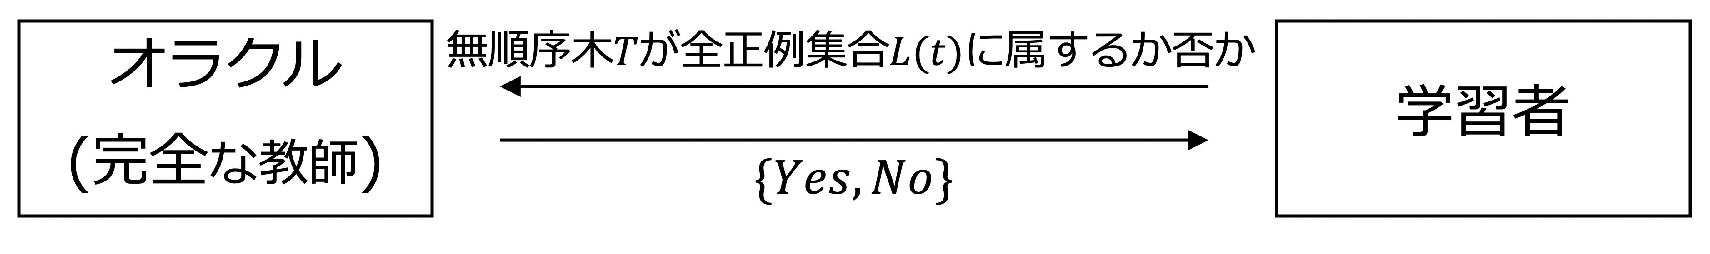
\includegraphics[scale=0.29]{fig/fig-ql_oracle.eps}
  \caption{線形無順序木パターンに対する所属性質問}\label{fig:ql_oracle}
\end{figure}

データセット$S$で学習したGCNを$GCN^S$とするとき,$GCN^S$をオラクルとする質問学習モデルを${\cal LUTP}$-${\cal QUERY}_{GCN^S}$とする.これは,質問学習の一連のプロセスにおいて,${\cal O}(t_{\ast})$を$GCN^S$に置き換え,GCNを活用して学習を協調的に進めるモデルである.これは無順序木を識別するための新しい形式のオラクルとして機能する.${\cal LUTP}$-${\cal QUERY}_{GCN^S}$でも,${\cal LUTP}$-${\cal QUERY}_{{\cal O}(t_{\ast})}$と同様に,正例の無順序木$T\in {\cal LUTP}$を入力とするとき,無順序木パターン$t$が1つだけ出力される.ただし,${\cal LUTP}$-${\cal QUERY}_{GCN^S}$は,不完全な教師であるため,$L(t_{\ast})=L(t)$となる無順序木パターン$t\in{\cal LUTP}$の同定に至らない可能性があることに注意する(図\ref{fig:ql_gcn}参照).

% 図4.2
\begin{figure}[tb]
  \centering
  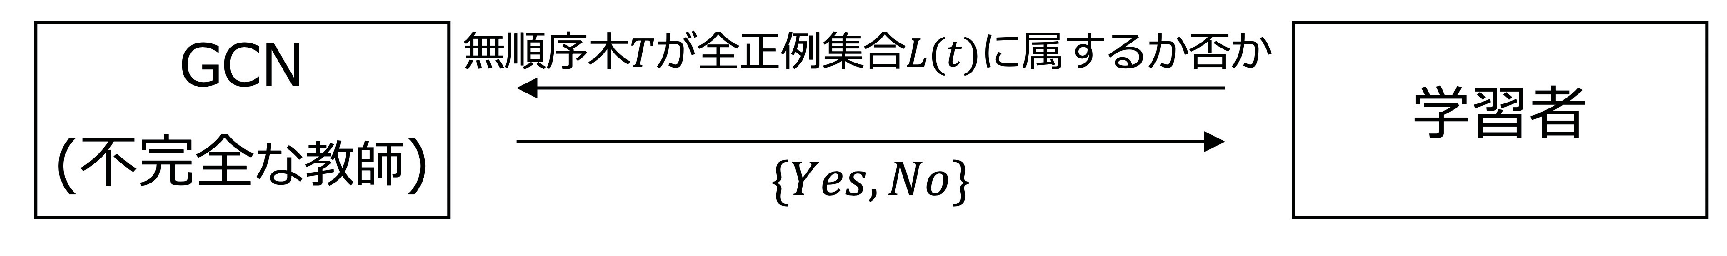
\includegraphics[scale=0.29]{fig/fig-ql_gcn.eps}
  \caption{GCNをオラクルとする線形無順序木パターンに対する所属性質問}\label{fig:ql_gcn}
\end{figure}

% 4.3
\subsection{実験的評価}
混同行列は,機械学習の分類問題において多く使われている評価指標で,TP(True Positive),FP(False Positive),FN(False Negative),TN(True Negative)を実際の値に対する予測の値の結果より分類される結果の値で表される.具体的には,各項\ref{subsec4.3.1}, \ref{subsec4.3.2}, \ref{subsec4.3.3}において定義する.

\textbf{再現率(recall)}とは,真の正例を正しく正例と予測した割合のことで,式(\ref{recall})で計算する.また,\textbf{適合率(precision)}とは,正例と予測したデータのうち真の正例の割合のことで,式(\ref{precision})で計算する.
\begin{equation}
  \label{recall}
  Recall=\frac{TP}{TP+FN},
\end{equation}
\begin{equation}
  \label{precision}
  Precision=\frac{TP}{TP+FP}.
\end{equation}

\textbf{F値(F1-score)}とは,再現率と適合率の調和平均である.F値は式(\ref{f1score})で計算する.本論文では,データセットの分類問題の評価指標としてF値を用いる.
\begin{equation}
  \label{f1score}
  F1 score=\frac{2\times Precision\times Recall}{Precicion+Recall}.
\end{equation}


% 4.3.1
\subsubsection{二値分類問題}\label{subsec4.3.1}
$S_+$と$S_-$を無順序木の集合とする.ただし,$S_+\cap S_-=\emptyset$と仮定する.$S_+^G$と$S_-^G$を$GCN^S$が$S$の無順序木をそれぞれ$S_+$と$S_-$に属すと予測した無順序木の集合とする.学習済みGCNの分類精度を$F$値($F_G$)で評価する.ここで,$TP=|S_+\cap S_+^G|$, $FP=|S_-\cap S_+^G|$, $FN=|S_+\cap S_-^G|$, $TN=|S_-\cap S_-^G|$である.これらを用いて,二値分類問題の再現率,適合率,$F$値をそれぞれ式(\ref{recallg}),(\ref{precisiong}),(\ref{f1scoreg})で算出する.
\begin{equation}
  \label{recallg}
  Recall_G=\frac{|S_+\cap S_+^G|}{|S_+|},
\end{equation}
\begin{equation}
  \label{precisiong}
  Precision_G=\frac{|S_+\cap S_+^G|}{|S_+^G|},
\end{equation}
\begin{equation}
  \label{f1scoreg}
  F_G=\frac{2\times Precision_G\times Recall_G}{Precision_G+Recall_G}.
\end{equation}


% 4.3.2
\subsubsection{無矛盾性問題}\label{subsec4.3.2}
$S_+$と$S_-$を次の条件を満たす${\cal UTP}_{\Sigma,\Lambda,X}$の有限部分集合とする:
無順序木パターン$t_{\ast}\in {\cal LUTP}_{\Sigma,\Lambda,X}$が存在して,$S_+\subset L(t_{\ast})$かつ$S_-\cap L(t_{\ast})=\emptyset$ である.ここでは,NP完全である${\cal LUTP}$-${\cal CP}$の計算問題として,$S_+\subset L(t)$かつ$S_-\cap L(t)=\emptyset$を満たす無順序木パターン$t$を出力する問題を考える.

無順序木$T\in S_+$に対して,${\cal LUTP}$-${\cal QUERY}_{GCN^S}(T)$の出力を$t_T$とする.$S_{+}^{Q(T)}=S\cap L(t_T)$,$S_{-}^{Q(T)}=S\setminus L(t_T)$とする.無順序木パターン$t_T$の精度を$F$値($F_{Q(T)}$)で評価する.ここで,$TP=|S_+\cap S_+^{Q(T)}|$, $FP=|S_-\cap S_+^{Q(T)}|$, $FN=|S_+\cap S_-^{Q(T)}|$, $TN=|S_-\cap S_-^{Q(T)}|$である.これらを用いて,無矛盾性問題の再現率,適合率,$F$値をそれぞれ式(\ref{recallq}),(\ref{precisionq}),(\ref{f1scoreq})で算出する.
\begin{equation}
  \label{recallq}
  Recall_{Q(T)}=\frac{|S_+\cap S_{+}^{Q(T)}|}{|S_+|},
\end{equation}
\begin{equation}
  \label{precisionq}
  Precision_{Q(T)}=\frac{|S_+\cap S_{+}^{Q(T)}|}{|S_{+}^{Q(T)}|},
\end{equation}
\begin{equation}
  \label{f1scoreq}
  F_{Q(T)}=\frac{2\times Precision_{Q(T)}\times Recall_{Q(T)}}{Precision_{Q(T)}+Recall_{Q(T)}}.
\end{equation}

\noindent
最後に式(\ref{fqmax})を達成する無順序木パターン$t$を出力する.
\begin{equation}
  \label{fqmax}
  F_Q=\max_{T\in S_+}F_{Q(T)}.
\end{equation}


% 4.3.3
\subsubsection{可視化問題}\label{subsec4.3.3}
$GCN^S$の可視化としての本手法の精度を,新たに生成した無順序木データ${S'}={S'}_+\cup {S'}_-$ $({S'}_+\cap {S'}_-=\emptyset)$を用いて,$F$値($F'_{GQ}$)で評価する.${S'}_+^G$と${S'}_-^G$を$GCN^S$が$S'$の無順序木をそれぞれ${S'}_+$と${S'}_-$に属すと予測した無順序木の集合とする.式(\ref{fqmax})を達成する無順序木パターン$t$に対して,${S'}_+^Q=S'\cap L(t)$,${S'}_-^Q=S'\setminus L(t)$とする.ここで,$TP=|{S'}_+^{G}\cap {S'}_+^{Q}|$, $FP=|{S'}_-^{G}\cap {S'}_+^{Q}|$, $FN=|{S'}_+^{G}\cap {S'}_-^{Q}|$, $TN=|{S'}_-^{G}\cap {S'}_-^{Q}|$である.これらを用いて,可視化問題の再現率,適合率,$F$値をそれぞれ式(\ref{recallgq}),(\ref{precisiongq}),(\ref{f1scoregq})で算出する.
\begin{equation}
  \label{recallgq}
  Recall'_{GQ}=\frac{|{S'}_+^G\cap {S'}_+^Q|}{|{S'}_+^G|},
\end{equation}
\begin{equation}
  \label{precisiongq}
  Precision'_{GQ}=\frac{|{S'}_+^G\cap {S'}_+^Q|}{|{S'}_+^Q|},
\end{equation}
\begin{equation}
  \label{f1scoregq}
  F'_{GQ}=\frac{2\times Precision'_{GQ}\times Recall'_{GQ}}{Precision'_{GQ}+Recall'_{GQ}}.
\end{equation}


% 4.4
\subsection{協調モデルの解析}
実験手順をアルゴリズム\ref{alg:exp_ql-gcn}に示す.計算機実験では,$\abs{S_+}=5000, \abs{S_-}=5000, \abs{S_L}=6400, \abs{S_V}=1600, \abs{S_T}=2000, \abs{S'}=10000$とし,この条件下で実験を行った.実験では,グラフ畳み込み層として(1)\,GraphConv,(2)\,RGCNConv,(3)\,GCNConvを使用し,質問学習アルゴリズムとして(a)\,${\cal LUTP}$-${\cal QUERY}_{GCN^S}^{Linear}$,(b)\,${\cal LUTP}$-${\cal QUERY}_{GCN^S}^{Square}$をそれぞれ使用し,これらの全ての組み合わせに対して計算機実験を実施した.それぞれ5487回の試行を繰り返し,安定した結果を得るようにした.GCNの学習においては,無順序木の各頂点$v$に与える初期の特徴ベクトルを,以下の7つの特徴量から構成した.

\begin{enumerate}
  \item[(i)] $v$の根からの深さ,
  \item[(ii)] $v$の子の数,
  \item[(iii)] $v$の子孫の数($v$から深さ2まで),
  \item[(iv)]$v$の子孫の数($v$から深さ3まで),
  \item[(v)] $v$の子孫の数($v$から深さ4まで),
  \item[(vi)] $v$の子孫の数,
  \item[(vii)] $v$の親への辺ラベルのone-hotベクトル,ただし,辺ラベル集合は$\Lambda=\{a,b,c,d,e\}$とする.
\end{enumerate}

% アルゴリズム8
\begin{algorithm}[tb]
\caption{GCNをオラクルとする質問学習(${\cal LUTP}$-${\cal QUERY}_{GCN^S}$)の実験手順;} \label{alg:exp_ql-gcn}
\begin{algorithmic}[1]
  \Require{$t_{\ast}\in {\cal LUTP}$;}
  \State $S\coloneqq S_+\cup S_-~(S_+\subset L(t_{\ast})\land S_-\cap L(t_{\ast})=\emptyset)$を生成;
  \State $GCN^S\coloneqq S$を学習データ$S_L$,検証データ$S_V$,テストデータ$S_T$に分割し$GCN^S$を構築;
  \State $Rec=\frac{|{S}_+\cap {S}_+^G|}{|{S}_+|}$,
      $Prec=\frac{|{S}_+\cap {S}_+^G|}{|{S}_+^G|}$,
      $F_G=\frac{2\times Prec\times Rec}{Prec+Rec}$;
  \For{$T\in S_+$}
    \State $t_T\coloneqq {\cal LUTP}$-${\cal QUERY}_{GCN^S}^{Linear}(T)$の出力;
    \State $Rec=\frac{|S_+\cap S_{+}^{Q_{Linear}(t_T)}|}{|S_+|}$,
    $Prec=\frac{|S_+\cap S_{+}^{Q_{Linear}(t_T)}|}{|S_{+}^{Q_{Linear}(t_T)}|}$,
    $F_{Q_{Linear}(t_T)}=\frac{2\times Prec\times Rec}{Prec+Rec}$;
    \State $t_T\coloneqq {\cal LUTP}$-${\cal QUERY}_{GCN^S}^{Square}(t_T)$の出力;
    \State $Rec=\frac{|S_+\cap S_{+}^{Q_{Square}(t_T)}|}{|S_+|}$,
    $Prec=\frac{|S_+\cap S_{+}^{Q_{Square}(t_T)}|}{|S_{+}^{Q_{Square}(t_T)}|}$,
    $F_{Q_{Square}(t_T)}=\frac{2\times Prec\times Rec}{Prec+Rec}$;
  \EndFor
  \State $F_{Q_{Linear}}\coloneqq \max_{T\in S_+}F_{Q(T)_{Linear}}$, $F_{Q_{Square}}\coloneqq \max_{T\in S_+}F_{Q(T)_{Square}}$;
  \State $t_{Linear}\coloneqq F_{Q_{Linear}}$を達成する無順序木パターン;
  \State $t_{Square}\coloneqq F_{Q_{Square}}$を達成する無順序木パターン;

  \State $S'\coloneqq S'_+\cup S'_-~(S'_+\subset L(t_{\ast})\land S'_-\cap L(t_{\ast})=\emptyset)$を生成;
  \State $Recall\coloneqq\frac{|{S'}_+\cap {S'}_+^G|}{|{S'}_+|}$,
      $Precision\coloneqq\frac{|{S'}_+\cap {S'}_+^G|}{|{S'}_+^G|}$,
      $F'_G\coloneqq\frac{2\times Precision\times Recall}{Precision+Recall}$;
    \For{$T\in S'_+$}
      \State $Rec\coloneqq\frac{|{S'}_+\cap {S'}_{+}^{Q_{Linear}(T)}|}{|{S'}_+|}$,
      $Prec\coloneqq\frac{|{S'}_+\cap {S'}_{+}^{Q_{Linear}(T)}|}{|{S'}_{+}^{Q_{Linear}(T)}|}$,
      $F_{Q_{Linear}(T)}\coloneqq\frac{2\times Prec\times Rec}{Prec+Rec}$;
      \State $Rec\coloneqq\frac{|{S'}_+\cap {S'}_{+}^{Q_{Square}(T)}|}{|{S'}_+|}$,
      $Prec\coloneqq\frac{|{S'}_+\cap {S'}_{+}^{Q_{Square}(T)}|}{|{S'}_{+}^{Q_{Square}(T)}|}$,
      $F_{Q_{Square}(T)}\coloneqq\frac{2\times Prec\times Rec}{Prec+Rec}$;
    \EndFor
  \State ${F'}_{Q_{Linear}}\coloneqq\max_{T\in {S'}_+}{F'}_{Q_{Linear}(T)}$;
  \State ${F'}_{Q_{Square}}\coloneqq\max_{T\in {S'}_+}{F'}_{Q_{Square}(T)}$;
  \State $Rec\coloneqq\frac{|{S'}_+^G\cap {S'}_+^{Q_{Linear}}|}{|{S'}_+^G|}$,
  $Prec\coloneqq\frac{|{S'}_+^G\cap {S'}_+^{Q_{Linear}}|}{|{S'}_+^{Q_{Linear}}|}$,
  $F'_{GQ_{Linear}}\coloneqq\frac{2\times Prec\times Rec}{Prec+Rec}$;
  \State $Rec\coloneqq\frac{|{S'}_+^G\cap {S'}_+^{Q_{Square}}|}{|{S'}_+^G|}$,
  $Prec\coloneqq\frac{|{S'}_+^G\cap {S'}_+^{Q_{Square}}|}{|{S'}_+^{Q_{Square}}|}$,
  $F'_{GQ_{Square}}\coloneqq\frac{2\times Prec\times Rec}{Prec+Rec}$;
\end{algorithmic}
\end{algorithm}

%実験結果を示す.
グラフ畳み込み層にGraphConvを使用した実験結果を図\ref{fig:result_graphconv}と表\ref{tbl:result_graphconv}に,RGCNConvを使用した実験結果を図\ref{fig:result_rgcnconv}と表\ref{tbl:result_rgcnconv}に,GCNConvを使用した実験結果を図\ref{fig:result_gcnconv}と表\ref{tbl:result_gcnconv}に示す.

% 図4.3
\begin{figure*}[tb]
  \centering
  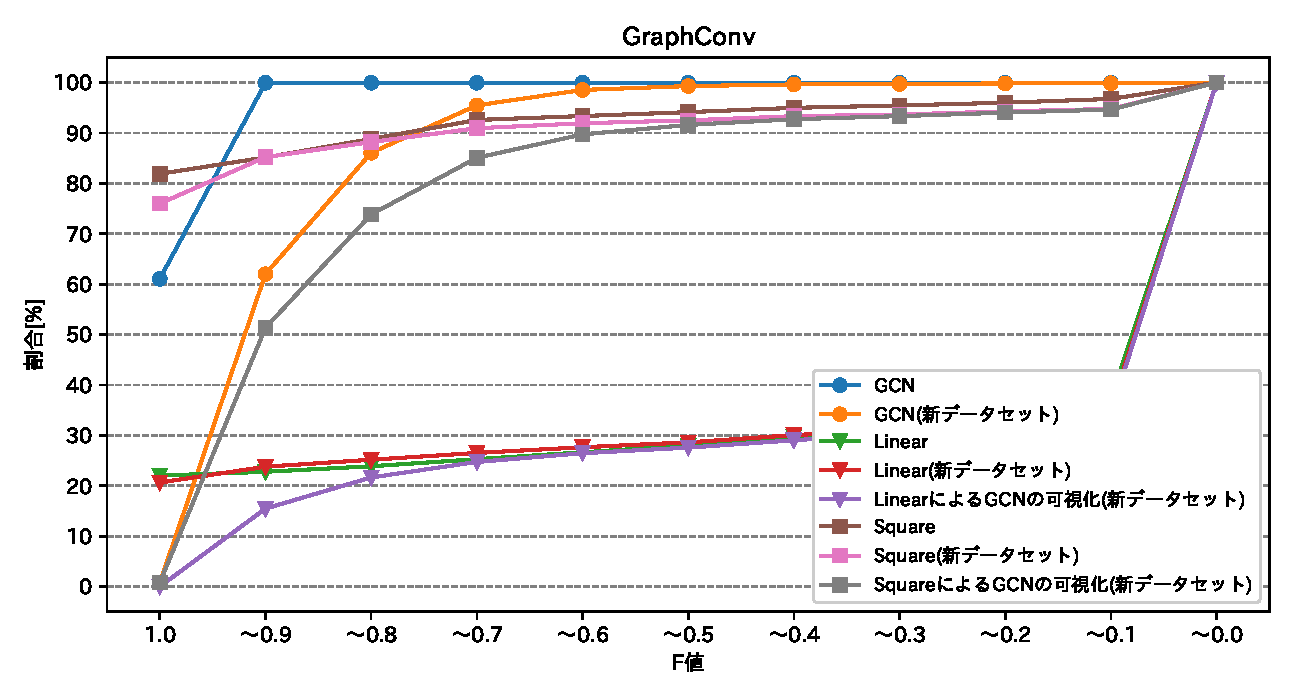
\includegraphics[scale=0.7]{fig/fig-exp_GraphConv.eps}
  \caption{横軸のF値超を達成した実験の割合(GraphConv)}\label{fig:result_graphconv}
\end{figure*}

% 表4.1
\begin{table*}[tb]
\caption{GraphConvの分類精度}\label{tbl:result_graphconv}
\centering
\begin{tabular}{|c|r|r|r|r|r|r|r|r|}\hline
  & \multicolumn{1}{|c|}{$F_{G}$} & \multicolumn{1}{|c|}{$F_{Q_{Linear}}$} & \multicolumn{1}{|c|}{$F_{Q_{Square}}$} & \multicolumn{1}{|c|}{$F'_{G}$} & \multicolumn{1}{|c|}{${F'}_{Q_{Linear}}$} & \multicolumn{1}{|c|}{${F'}_{Q_{Square}}$} & \multicolumn{1}{|c|}{${F'}_{GQ_{Linear}}$} & \multicolumn{1}{|c|}{${F'}_{GQ_{Square}}$}\\
  \hline
  \multicolumn{1}{|c|}{F値} & \multicolumn{1}{|c|}{割合} & \multicolumn{1}{|c|}{割合} & \multicolumn{1}{|c|}{割合} & \multicolumn{1}{|c|}{割合} & \multicolumn{1}{|c|}{割合} & \multicolumn{1}{|c|}{割合} & \multicolumn{1}{|c|}{割合} & \multicolumn{1}{|c|}{割合} \\
  \hline
  1.0   & 61.1 & 22.0 & 81.9 & 0.8 & 20.6 & 76.0 & 0.0 & 0.8 \\
  〜0.9 & 100.0 & 22.8 & 85.1 & 62.0 & 23.8 & 85.2 & 15.5 & 51.4 \\
  〜0.8 & 100.0 & 23.9 & 88.8 & 86.1 & 25.2 & 88.2 & 21.7 & 73.8 \\
  〜0.7 & 100.0 & 25.3 & 92.6 & 95.5 & 26.5 & 90.9 & 24.7 & 85.1 \\
  〜0.6 & 100.0 & 26.6 & 93.4 & 98.5 & 27.6 & 91.9 & 26.5 & 89.7 \\
  〜0.5 & 100.0 & 28.0 & 94.1 & 99.3 & 28.6 & 92.5 & 27.6 & 91.6 \\
  〜0.4 & 100.0 & 29.8 & 95.0 & 99.6 & 30.1 & 93.3 & 29.0 & 92.7 \\
  〜0.3 & 100.0 & 31.3 & 95.5 & 99.7 & 31.1 & 93.7 & 30.5 & 93.3 \\
  〜0.2 & 100.0 & 33.0 & 96.0 & 99.8 & 32.1 & 94.3 & 31.8 & 94.0 \\
  〜0.1 & 100.0 & 37.3 & 96.8 & 99.9 & 35.4 & 94.8 & 34.5 & 94.7 \\
  〜0.0 & 100.0 & 100.0 & 100.0 & 100.0 & 100.0 & 100.0 & 100.0 & 100.0 \\
  \hline
\end{tabular}
\end{table*}

% 図4.4
\begin{figure*}[tb]
  \centering
  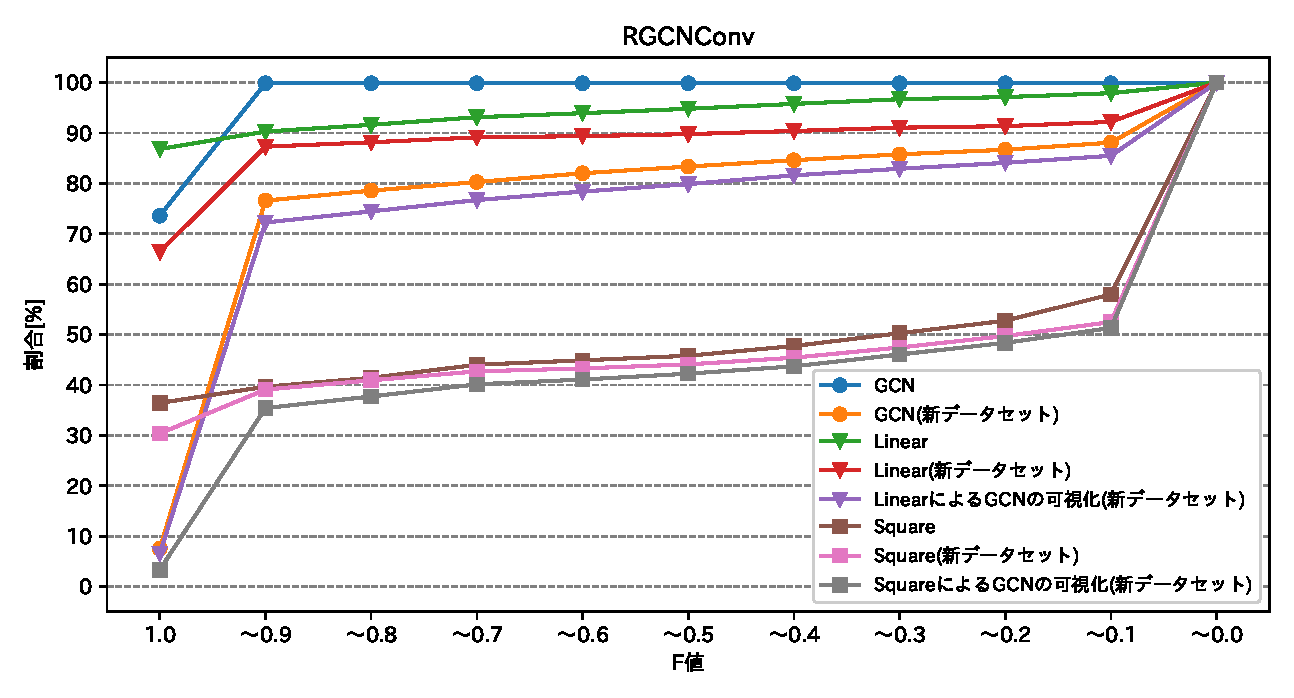
\includegraphics[scale=0.7]{fig/fig-exp_RGCNConv.eps}
  \caption{横軸のF値超を達成した実験の割合(RGCNConv)}\label{fig:result_rgcnconv}
\end{figure*}

% 表4.2
\begin{table*}[tb]
\caption{RGCNConvの分類精度}\label{tbl:result_rgcnconv}
\centering
\begin{tabular}{|c|r|r|r|r|r|r|r|r|}\hline
  & \multicolumn{1}{|c|}{$F_{G}$} & \multicolumn{1}{|c|}{$F_{Q_{Linear}}$} & \multicolumn{1}{|c|}{$F_{Q_{Square}}$} & \multicolumn{1}{|c|}{$F'_{G}$} & \multicolumn{1}{|c|}{${F'}_{Q_{Linear}}$} & \multicolumn{1}{|c|}{${F'}_{Q_{Square}}$} & \multicolumn{1}{|c|}{${F'}_{GQ_{Linear}}$} & \multicolumn{1}{|c|}{${F'}_{GQ_{Square}}$}\\
  \hline
  \multicolumn{1}{|c|}{F値} & \multicolumn{1}{|c|}{割合} & \multicolumn{1}{|c|}{割合} & \multicolumn{1}{|c|}{割合} & \multicolumn{1}{|c|}{割合} & \multicolumn{1}{|c|}{割合} & \multicolumn{1}{|c|}{割合} & \multicolumn{1}{|c|}{割合} & \multicolumn{1}{|c|}{割合} \\
  \hline
  1.0   & 73.6 & 86.8 & 36.4 & 7.5 & 66.4 & 30.4 & 6.5 & 3.3 \\
  〜0.9 & 99.9 & 90.3 & 39.7 & 76.6 & 87.3 & 39.1 & 72.2 & 35.4 \\
  〜0.8 & 99.9 & 91.6 & 41.4 & 78.6 & 88.2 & 40.9 & 74.4 & 37.7 \\
  〜0.7 & 99.9 & 93.1 & 44.0 & 80.3 & 89.1 & 42.7 & 76.7 & 40.1 \\
  〜0.6 & 99.9 & 93.9 & 44.9 & 82.0 & 89.4 & 43.3 & 78.4 & 41.1 \\
  〜0.5 & 99.9 & 94.8 & 45.8 & 83.3 & 89.8 & 44.1 & 79.9 & 42.2 \\
  〜0.4 & 99.9 & 95.8 & 47.7 & 84.6 & 90.4 & 45.4 & 81.6 & 43.7 \\
  〜0.3 & 99.9 & 96.7 & 50.3 & 85.8 & 91.1 & 47.4 & 82.9 & 46.1 \\
  〜0.2 & 99.9 & 97.1 & 52.7 & 86.7 & 91.4 & 49.7 & 84.1 & 48.4 \\
  〜0.1 & 99.9 & 97.9 & 58.0 & 88.1 & 92.2 & 52.5 & 85.5 & 51.3 \\
  〜0.0 & 100.0 & 100.0 & 100.0 & 100.0 & 100.0 & 100.0 & 100.0 & 100.0 \\
  \hline
\end{tabular}
\end{table*}

% 図4.5
\begin{figure*}[tb]
  \centering
  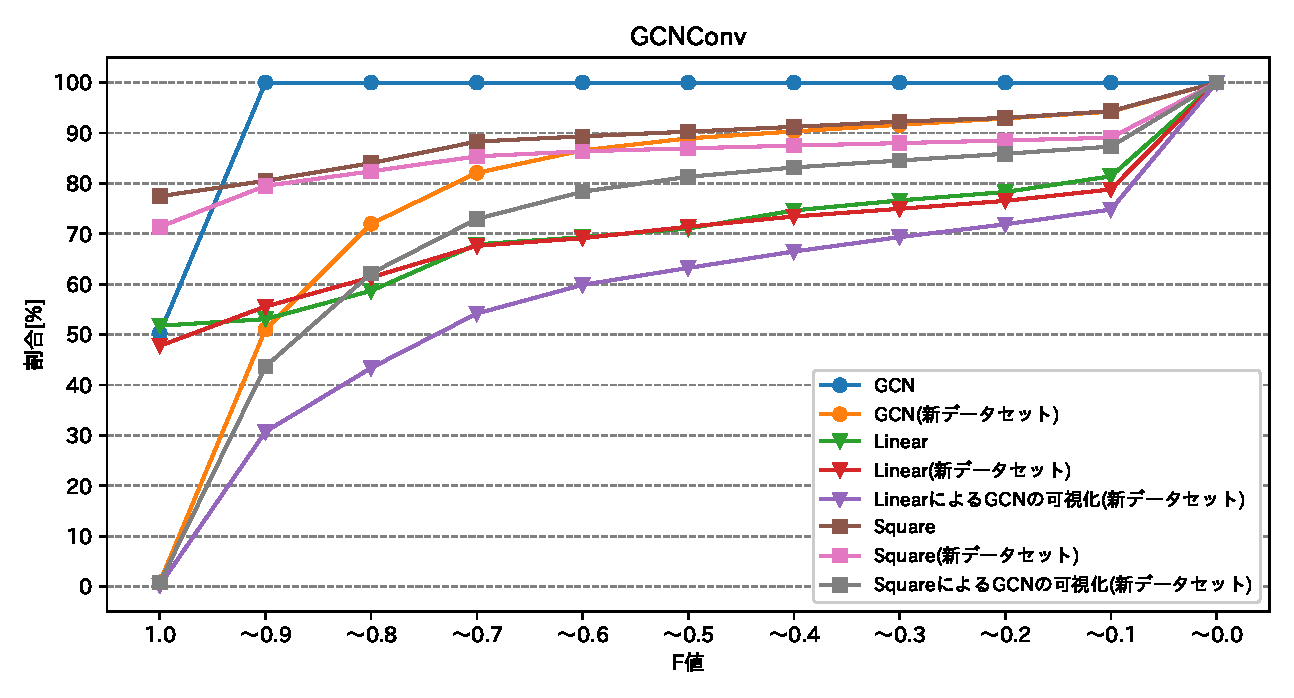
\includegraphics[scale=0.7]{fig/fig-exp_GCNConv.eps}
  \caption{横軸のF値超を達成した実験の割合(GCNConv)}\label{fig:result_gcnconv}
\end{figure*}

% 表4.3
\begin{table*}[tb]
\caption{GCNConvの分類精度}\label{tbl:result_gcnconv}
\centering
\begin{tabular}{|c|r|r|r|r|r|r|r|r|}\hline
  & \multicolumn{1}{|c|}{$F_{G}$} & \multicolumn{1}{|c|}{$F_{Q_{Linear}}$} & \multicolumn{1}{|c|}{$F_{Q_{Square}}$} & \multicolumn{1}{|c|}{$F'_{G}$} & \multicolumn{1}{|c|}{${F'}_{Q_{Linear}}$} & \multicolumn{1}{|c|}{${F'}_{Q_{Square}}$} & \multicolumn{1}{|c|}{${F'}_{GQ_{Linear}}$} & \multicolumn{1}{|c|}{${F'}_{GQ_{Square}}$}\\
  \hline
  \multicolumn{1}{|c|}{F値} & \multicolumn{1}{|c|}{割合} & \multicolumn{1}{|c|}{割合} & \multicolumn{1}{|c|}{割合} & \multicolumn{1}{|c|}{割合} & \multicolumn{1}{|c|}{割合} & \multicolumn{1}{|c|}{割合} & \multicolumn{1}{|c|}{割合} & \multicolumn{1}{|c|}{割合} \\
  \hline
  1.0   & 50.2 & 51.8 & 77.5 & 0.9 & 47.8 & 71.4 & 0.2 & 0.8 \\
  〜0.9 & 100.0 & 53.1 & 80.5 & 51.0 & 55.6 & 79.5 & 30.7 & 43.7 \\
  〜0.8 & 100.0 & 58.7 & 84.0 & 72.0 & 61.4 & 82.4 & 43.4 & 62.1 \\
  〜0.7 & 100.0 & 67.9 & 88.3 & 82.1 & 67.6 & 85.4 & 54.2 & 72.9 \\
  〜0.6 & 100.0 & 69.3 & 89.3 & 86.6 & 69.1 & 86.4 & 59.9 & 78.3 \\
  〜0.5 & 100.0 & 71.0 & 90.3 & 88.9 & 71.4 & 87.0 & 63.2 & 81.3 \\
  〜0.4 & 100.0 & 74.6 & 91.2 & 90.3 & 73.4 & 87.5 & 66.5 & 83.2 \\
  〜0.3 & 100.0 & 76.6 & 92.3 & 91.6 & 75.0 & 88.0 & 69.3 & 84.5 \\
  〜0.2 & 100.0 & 78.3 & 93.0 & 92.9 & 76.5 & 88.5 & 71.9 & 85.9 \\
  〜0.1 & 100.0 & 81.4 & 94.3 & 94.2 & 78.8 & 89.1 & 74.8 & 87.3 \\
  〜0.0 & 100.0 & 100.0 & 100.0 & 100.0 & 100.0 & 100.0 & 100.0 & 100.0 \\
  \hline
\end{tabular}
\end{table*}

%% 結果・考察
\subsection{協調モデルの解析に関する考察}
%$F$値の評価基準として,0.9を超えれば高精度,0.1以下であれば低精度とみなす.
%結果より,GraphConvに関して,高精度で分類することのできる線形無順序木パターンを,${\cal LUTP}$-${\cal QUERY}_{GCN^S}^{Linear}$では全実験5487回のうち22.8\%,${\cal LUTP}$-${\cal QUERY}_{GCN^S}^{Square}$では85.1\%の割合で発見することができた.一方で,RGCNConvに関して高精度で分類することのできる線形無順序木パターンを,${\cal LUTP}$-${\cal QUERY}_{GCN^S}^{Linear}$では90.3\%,${\cal LUTP}$-${\cal QUERY}_{GCN^S}^{Square}$では39.7\%の割合で発見することができた.このことから,GraphConvは${\cal LUTP}$-${\cal QUERY}_{GCN^S}^{Square}$を得意とし,RGCNConvは${\cal LUTP}$-${\cal QUERY}_{GCN^S}^{Linear}$を得意とすることが確認できる.これは,GraphConvは近接する頂点間の特徴,RGCNConvは同じ辺ラベルの特徴を捉えているからであると考えられる.
%
%次に学習の際に使用したデータセット$S$と新しいデータセット$S'$の比較を行う.精度の高かった(GraphConv, ${\cal LUTP}$-${\cal QUERY}_{GCN^S}^{Square}$),(RGCNConv, ${\cal LUTP}$-${\cal QUERY}_{GCN^S}^{Linear}$)ともに$F_G=1.0$であった実験の割合と$F'_G=1.0$の割合の差が著しい.このことから学習済みGCNは過学習を起こしている可能性が高いと言える.一方で,質問学習によって発見された線形無順序木パターンは,どちらのグラフ畳み込み層でも$F_G=1.0$であった実験の割合と$F'_G=1.0$の割合の差が小さい.このことは発見された線形無順序木パターンでは過学習を起こしにくいということを示唆している.過学習を起こしにくいことの理由の一つとして,線形無順序木パターンに対する質問学習モデルが無順序木であることを前提に行われていることがあげられる.
%
%中間層の特徴と使用するアルゴリズムの特徴によって顕著な差があることがわかった.そこで,相関関係について調査を行った.まず,任意のF値以上を達成した線形無順序木パターンの集合を$P$,達成できなかった集合を$N$とし,それぞれの線形無順序木パターンの葉のうち変数である割合を調べた.結果を表\ref{tbl:variable_ratio}に示す.結果より,F値と葉のうち変数である割合の間に相関は見られなかった.

%実験結果を3つの計算問題と照らし合わせてみる.%$F$値の評価基準として,0.9を超えれば高精度,0.1以下であれば低精度とみなすこととする.
\subsubsection*{二値分類問題に関する考察}
二値分類問題に関しては,$F_G$が0.9以上を獲得できた実験が全実験5487回のうち,GraphConvでは100.0\%,RGCNConvでは99.9\%,GCNConvでは100.0\%と,いずれのグラフ畳み込み層を使用した場合においても,非常に高い分類精度が達成されることが確認された.一方で,新しいデータセットでの分類精度$F'_G$は,GraphConvでは62.0\%,RGCNConvでは76.6\%,GCNConvでは51.0\%と大きく低下しており,学習データに依存した過学習が発生している可能性が示唆される.

\subsubsection*{無矛盾性問題に関する考察}
無矛盾性問題に関しては,使用するグラフ畳み込み層と質問学習アルゴリズムの組み合わせによって顕著な差が確認される.GraphConvを使用した場合,$F_{Q_{Linear}}$と$F_{Q_{Square}}$に対して0.9以上を獲得できた実験が全実験5487回のうち,アルゴリズム${\cal LUTP}$-${\cal QUERY}_{GCN^S}^{Linear}$で得られた線形無順序木パターンの分類精度$F_{Q_{Linear}}$は22.8\%にとどまった.一方,${\cal LUTP}$-${\cal QUERY}_{GCN^S}^{Square}$では85.1\%と大幅に高い分類精度$F_{Q_{Square}}$が達成されており,両アルゴリズム間で明確な差が見られる.さらに,図\ref{fig:result_graphconv}全体を確認すると,${\cal LUTP}$-${\cal QUERY}_{GCN^S}^{Linear}$による結果は図の下側を中心に位置している一方,${\cal LUTP}$-${\cal QUERY}_{GCN^S}^{Square}$の結果は図の上側を中心に位置していることがわかる.これらの結果は,GraphConvを用いた場合,アルゴリズム${\cal LUTP}$-${\cal QUERY}_{GCN^S}^{Square}$の方が学習効果が高いことを示している.RGCNConvを使用した場合,アルゴリズム${\cal LUTP}$-${\cal QUERY}_{GCN^S}^{Linear}$で得られた線形無順序木パターンの分類精度$F_{Q_{Linear}}$は90.3\%と非常に高精度である.一方,${\cal LUTP}$-${\cal QUERY}_{GCN^S}^{Square}$では39.7\%と低精度であり,RGCNConvを用いた場合でも両アルゴリズムで明確な差が見られる.さらに,図\ref{fig:result_rgcnconv}全体を確認すると,${\cal LUTP}$-${\cal QUERY}_{GCN^S}^{Linear}$による結果は図の上側を中心に位置している一方,${\cal LUTP}$-${\cal QUERY}_{GCN^S}^{Square}$の結果は図の下側を中心に位置している.これらの結果は,RGCNConvを用いた場合,アルゴリズム${\cal LUTP}$-${\cal QUERY}_{GCN^S}^{Linear}$の方が学習効果が高いことを示している.GCNConvでは,GraphConvやRGCNConvにおけるような大きな差は確認されていない.

\subsubsection*{可視化問題に関する考察}
可視化問題に関しては,無矛盾性問題と同様の傾向が確認される.具体的には,グラフ畳み込み層GraphConvでは,アルゴリズム${\cal LUTP}$-${\cal QUERY}_{GCN^S}^{Square}$の方が高い精度${F'}_{GQ_{Square}}$でGCNの予測根拠を可視化している.一方でRGCNConvでは,${\cal LUTP}$-${\cal QUERY}_{GCN^S}^{Linear}$の方が高い精度${F'}_{GQ_{Linear}}$でGCNの予測根拠を可視化していることが確認された.これらの結果は,GraphConvでは${\cal LUTP}$-${\cal QUERY}_{GCN^S}^{Square}$の方が,RGCNConvでは${\cal LUTP}$-${\cal QUERY}_{GCN^S}^{Linear}$の方が学習効果に優れており,分類精度の高い線形無順序木パターンを獲得することが可能であるため,GCNの予測根拠を可視化できていると考えられる.これらの結果から,GraphConvを使用した場合はアルゴリズム${\cal LUTP}$-${\cal QUERY}_{{\cal O}(t)}^{Square}$の精度が高く,RGCNConvを使用した場合はアルゴリズム${\cal LUTP}$-${\cal QUERY}_{{\cal O}(t)}^{Linear}$の精度が高いことが確認される.この違いは,使用するグラフ畳み込み層の特徴に起因していると考えられる.具体的には,GraphConvが隣接する頂点数に基づいて特徴を集約するのに対し,RGCNConvが辺ラベルの種類に基づいて特徴を集約するという両者の特性の違いがあり,それがGCNの学習効果に影響を与えていると考えられる.

% 表4.4
\begin{table*}[tb]
\caption{F値と変数の割合の関係}\label{tbl:variable_ratio}
\centering
\begin{tabular}{|c|rr|rr|rr|rr|rr|rr|}\hline
  \multicolumn{7}{|c|}{${\cal LUTP}$-${\cal QUERY}_{GCN^S}^{Linear}$} \\ \hline
  \multirow{2}{*}{F値} & \multicolumn{2}{|c|}{GraphConv} & \multicolumn{2}{|c|}{RGCNConv} & \multicolumn{2}{|c|}{GCNConv} \\ \cline{2-7}
  & P: 変数の割合 & N: 変数の割合 & P: 変数の割合 & N: 変数の割合 & P: 変数の割合 & N: 変数の割合 \\ \hline
  0.9 &   0.65479 &       0.44864 &       0.48297 &       0.61297 &       0.51224 &       0.47678 \\
  0.8 &   0.65618 &       0.44524 &       0.48568 &       0.60398 &       0.51343 &       0.47028 \\
  0.7 &   0.65786 &       0.44071 &       0.48811 &       0.59711 &       0.49702 &       0.49260 \\
  0.6 &   0.66183 &       0.43522 &       0.49024 &       0.57854 &       0.50064 &       0.48422 \\
  0.5 &   0.66332 &       0.43046 &       0.49199 &       0.56143 &       0.50260 &       0.47843 \\
  0.4 &   0.66015 &       0.42582 &       0.49272 &       0.56097 &       0.49799 &       0.48857 \\
  0.3 &   0.65904 &       0.42116 &       0.49446 &       0.52904 &       0.49900 &       0.48447 \\
  0.2 &   0.65975 &       0.41460 &       0.49543 &       0.50154 &       0.50081 &       0.47680 \\
  0.1 &   0.64320 &       0.40777 &       0.49629 &       0.46327 &       0.50252 &       0.46532 \\ \hline\hline
  \multicolumn{7}{|c|}{${\cal LUTP}$-${\cal QUERY}_{GCN^S}^{Square}$} \\ \hline
  0.9 &   0.47923 &       0.58944 &       0.44011 &       0.53207 &       0.46454 &       0.62384 \\
  0.8 &   0.48282 &       0.59703 &       0.44477 &       0.53155 &       0.46933 &       0.63387 \\
  0.7 &   0.48665 &       0.60732 &       0.44288 &       0.53705 &       0.47379 &       0.66021 \\
  0.6 &   0.48858 &       0.59438 &       0.44651 &       0.53559 &       0.47669 &       0.65409 \\
  0.5 &   0.48975 &       0.58943 &       0.45066 &       0.53358 &       0.47868 &       0.65255 \\
  0.4 &   0.49037 &       0.59473 &       0.45211 &       0.53532 &       0.47985 &       0.65921 \\
  0.3 &   0.49103 &       0.59171 &       0.45328 &       0.53837 &       0.48193 &       0.65842 \\
  0.2 &   0.49176 &       0.58812 &       0.45463 &       0.54133 &       0.48337 &       0.65775 \\
  0.1 &   0.49282 &       0.57859 &       0.46779 &       0.53397 &       0.48694 &       0.63974 \\ \hline
\end{tabular}
\end{table*}

\subsubsection*{精度と精度以外の相関関係に関する考察}
計算機実験ではランダムに生成した線形無順序木パターンを用いているが,協調モデルによって出力される線形無順序木パターンには精度が高いものと低いものが存在することが確認される.そこで,精度と精度以外の数値の相関関係について調査する.
まず,各F値に対して質問回数の多少について調査を行う.使用したGCNのグラフ畳み込み層と質問アルゴリズムのペアを順序対で表す.(GraphConv, ${\cal LUTP}$-${\cal QUERY}_{GCN^S}^{Linear}$)の結果を図\ref{fig:GraphConv_ln_ql_f1_nodes}に,(GraphConv, ${\cal LUTP}$-${\cal QUERY}_{GCN^S}^{Square}$)の結果を図\ref{fig:GraphConv_sqr_ql_f1_nodes}に,(RGCNConv, ${\cal LUTP}$-${\cal QUERY}_{GCN^S}^{Linear}$)の結果を図\ref{fig:RGCNConv_ln_ql_f1_nodes}に,(RGCNConv, ${\cal LUTP}$-${\cal QUERY}_{GCN^S}^{Square}$)の結果を図\ref{fig:RGCNConv_sqr_ql_f1_nodes}に,(GCNConv, ${\cal LUTP}$-${\cal QUERY}_{GCN^S}^{Linear}$)の結果を図\ref{fig:GCNConv_ln_ql_f1_nodes}に,(GCNConv, ${\cal LUTP}$-${\cal QUERY}_{GCN^S}^{Square}$)の結果を図\ref{fig:GCNConv_sqr_ql_f1_nodes}に示す.いずれの結果もF値と質問回数の間に相関は見られない.さらに,正例の総頂点数を加えて調査する.この調査では,質問回数と頂点数の間に正の相関が見られる.これは,正例の頂点数が質問回数に影響を与えることであり,自明な結果である.

% 図4.6
\begin{figure*}[tb]
  \centering
  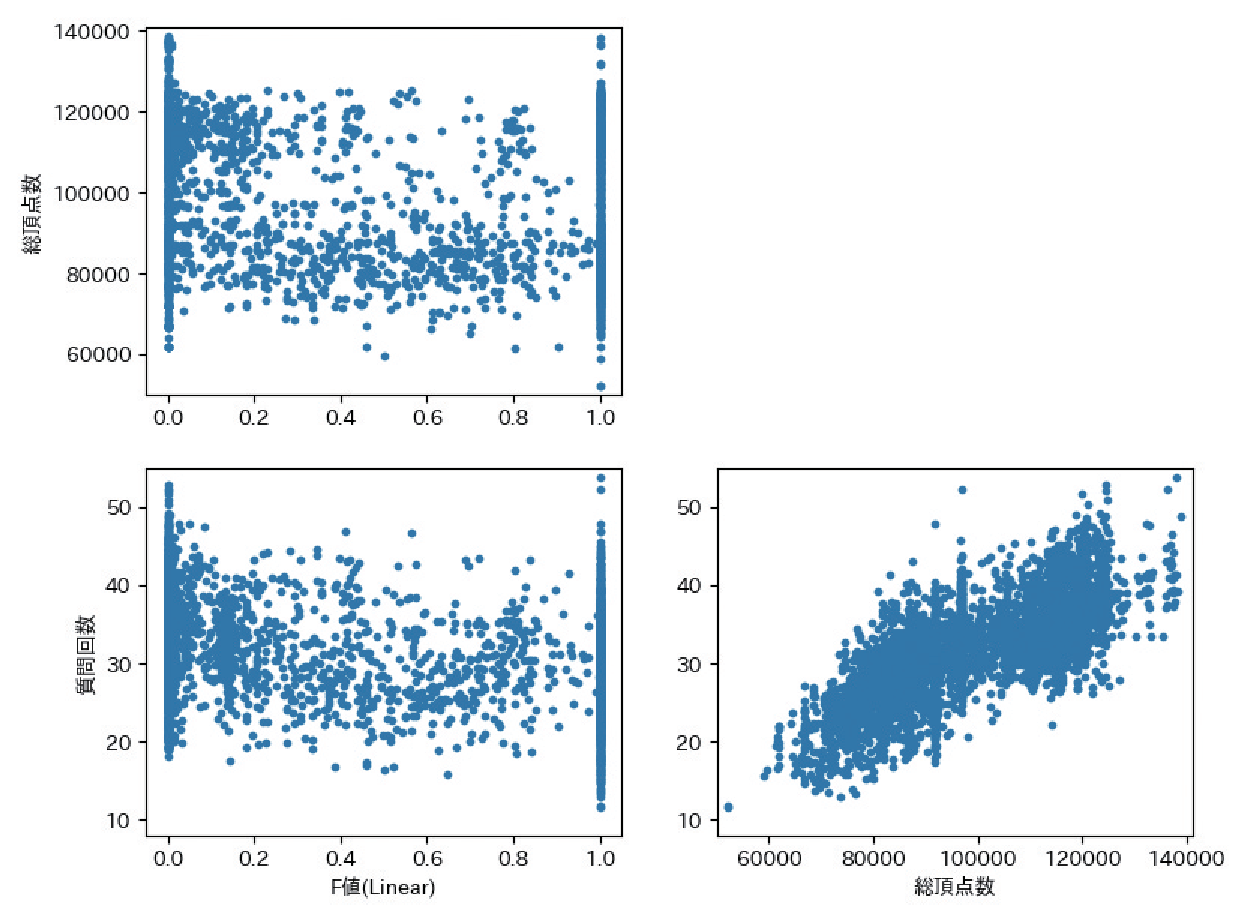
\includegraphics[scale=0.66]{fig/fig-GraphConv_ln_ql_f1_nodes.eps}
  \caption{グラフ畳み込み層にGraphConvを,質問学習アルゴリズムに${\cal LUTP}$-${\cal QUERY}_{GCN^S}^{Linear}$を使用し,F値と質問回数と無順序木パターンの正例の総頂点数による解析結果}\label{fig:GraphConv_ln_ql_f1_nodes}
\end{figure*}

% 図4.7
\begin{figure*}[tb]
  \centering
  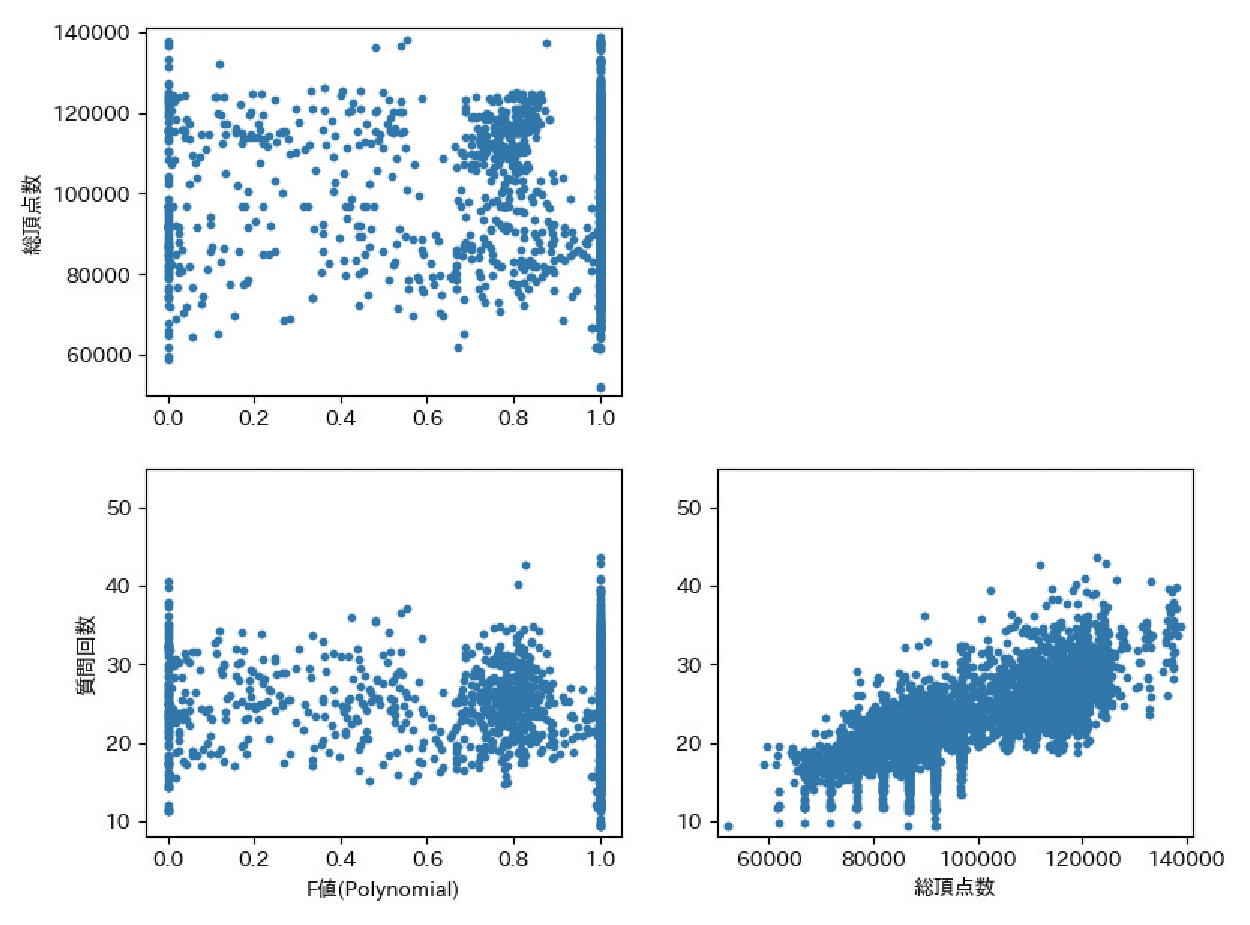
\includegraphics[scale=0.66]{fig/fig-GraphConv_sqr_ql_f1_nodes.eps}
  \caption{グラフ畳み込み層にGraphConvを,質問学習アルゴリズムに${\cal LUTP}$-${\cal QUERY}_{GCN^S}^{Square}$を使用し,F値と質問回数と無順序木パターンの正例の総頂点数による解析結果}\label{fig:GraphConv_sqr_ql_f1_nodes}
\end{figure*}

% 図4.8
\begin{figure*}[tb]
  \centering
  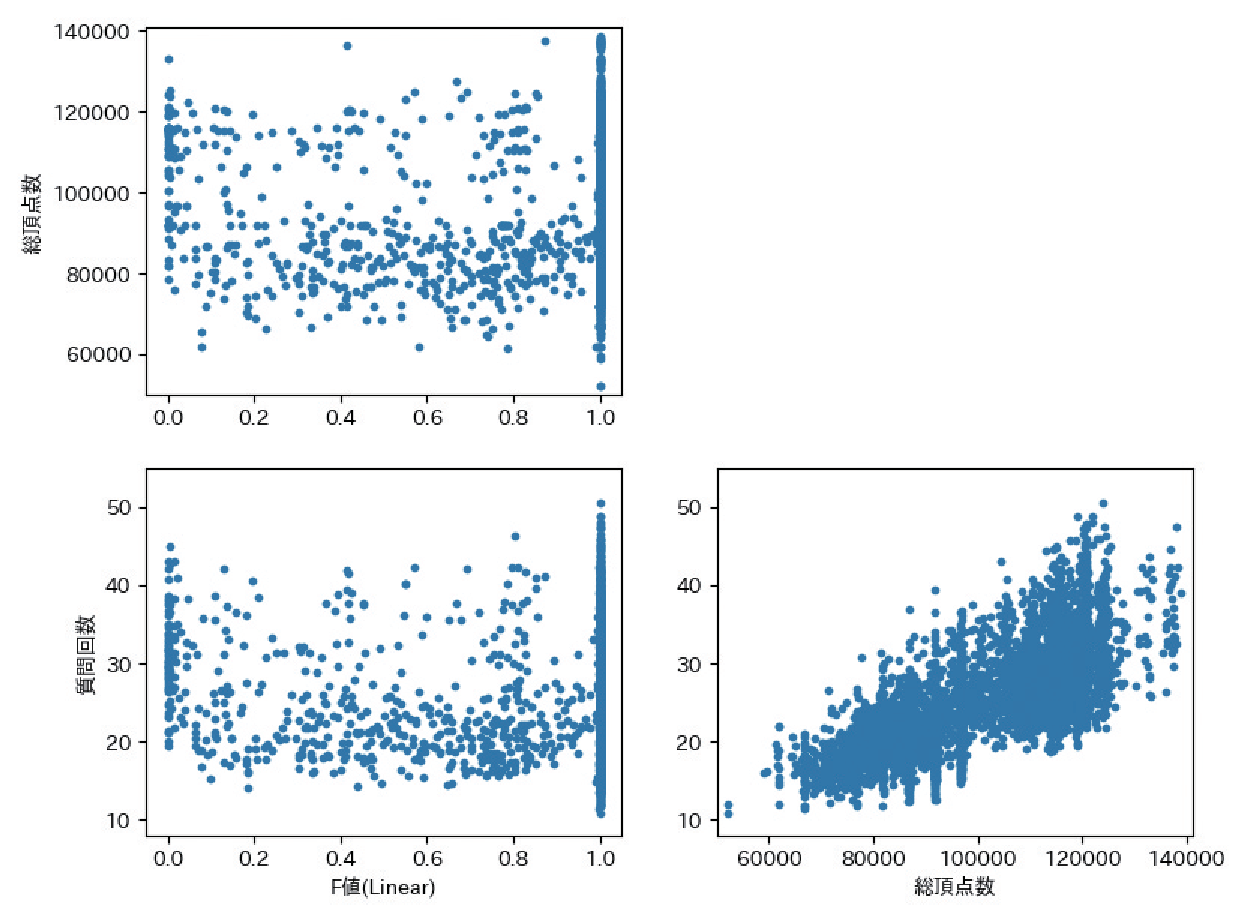
\includegraphics[scale=0.66]{fig/fig-RGCNConv_ln_ql_f1_nodes.eps}
  \caption{グラフ畳み込み層にRGCNConvを,質問学習アルゴリズムに${\cal LUTP}$-${\cal QUERY}_{GCN^S}^{Linear}$を使用し,F値と質問回数と無順序木パターンの正例の総頂点数による解析結果}\label{fig:RGCNConv_ln_ql_f1_nodes}
\end{figure*}

% 図4.9
\begin{figure*}[tb]
  \centering
  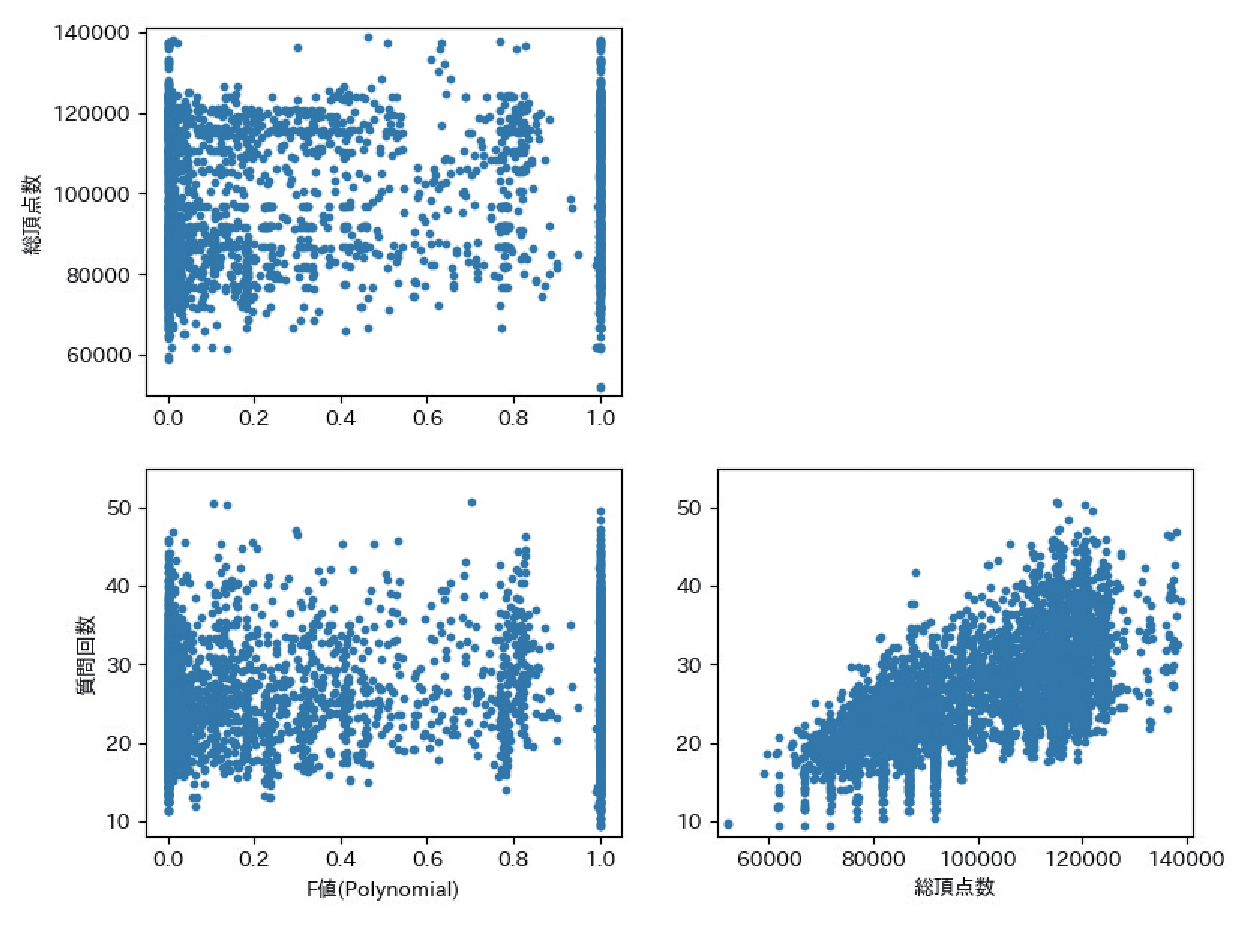
\includegraphics[scale=0.66]{fig/fig-RGCNConv_sqr_ql_f1_nodes.eps}
  \caption{グラフ畳み込み層にRGCNConvを,質問学習アルゴリズムに${\cal LUTP}$-${\cal QUERY}_{GCN^S}^{Square}$を使用し,F値と質問回数と無順序木パターンの正例の総頂点数による解析結果}\label{fig:RGCNConv_sqr_ql_f1_nodes}
\end{figure*}

% 図4.10
\begin{figure*}[tb]
  \centering
  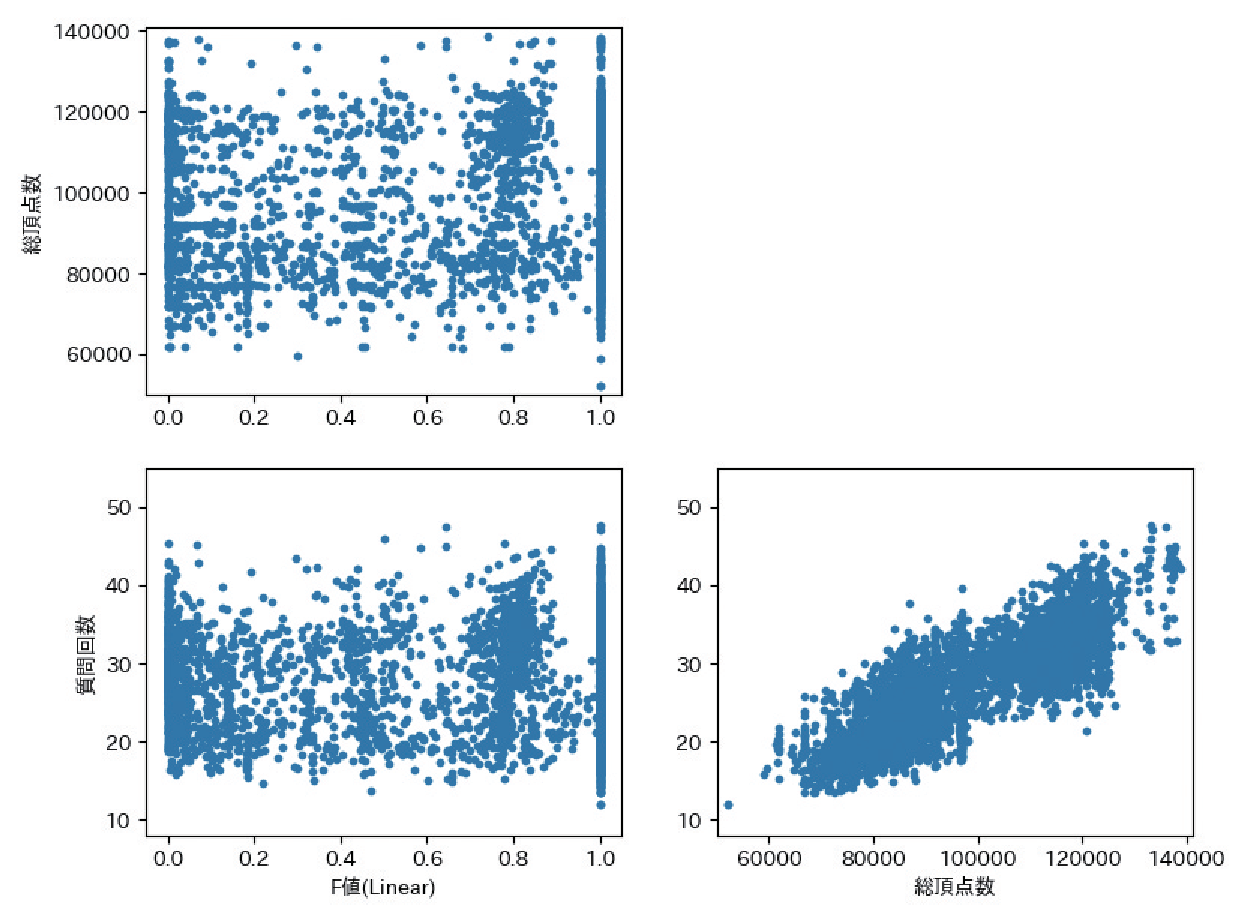
\includegraphics[scale=0.66]{fig/fig-GCNConv_ln_ql_f1_nodes.eps}
  \caption{グラフ畳み込み層にGCNConvを,質問学習アルゴリズムに${\cal LUTP}$-${\cal QUERY}_{GCN^S}^{Linear}$を使用し,F値と質問回数と無順序木パターンの正例の総頂点数による解析結果}\label{fig:GCNConv_ln_ql_f1_nodes}
\end{figure*}

% 図4.11
\begin{figure*}[tb]
  \centering
  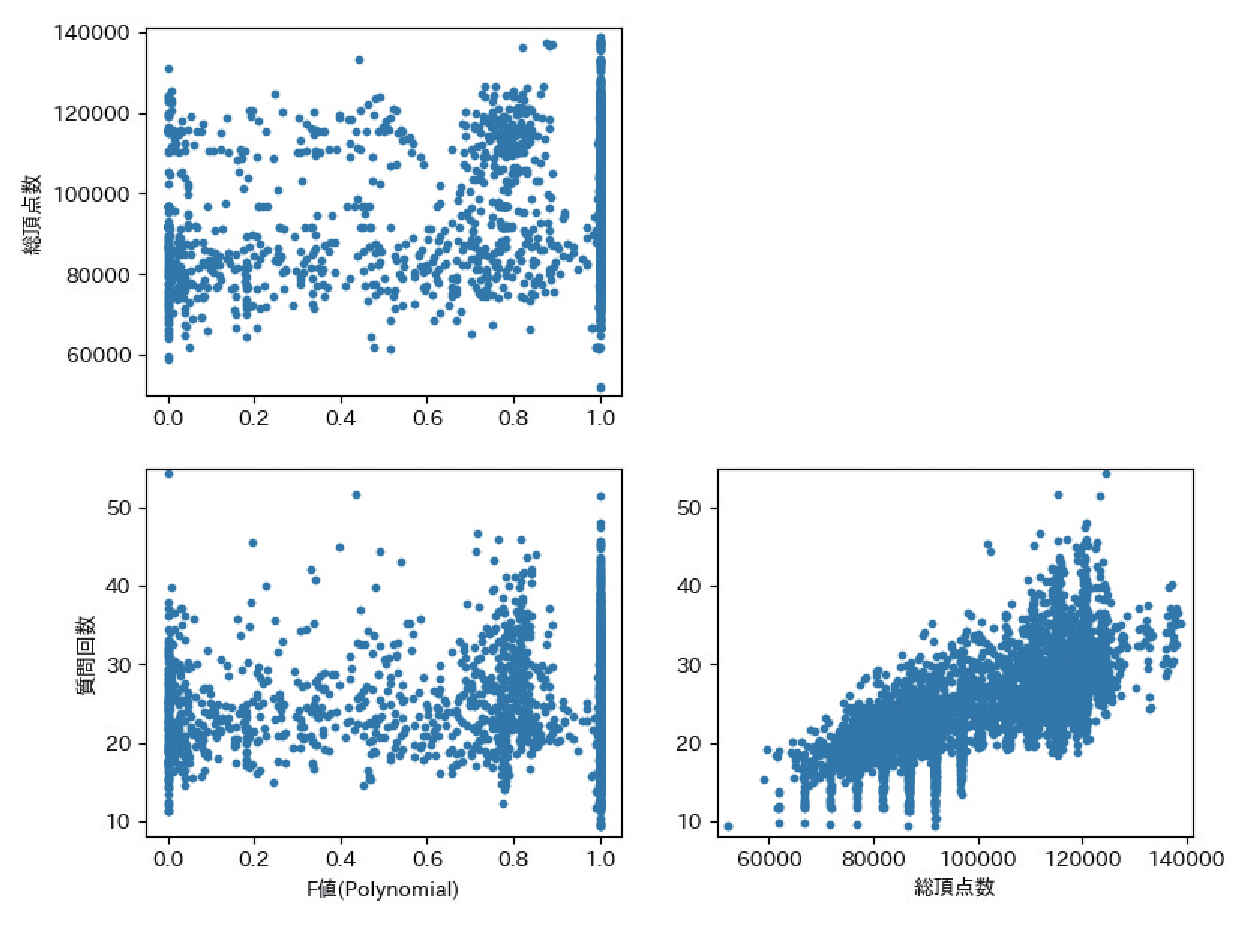
\includegraphics[scale=0.66]{fig/fig-GCNConv_sqr_ql_f1_nodes.eps}
  \caption{グラフ畳み込み層にGCNConvを,質問学習アルゴリズムに${\cal LUTP}$-${\cal QUERY}_{GCN^S}^{Square}$を使用し,F値と質問回数と無順序木パターンの正例の総頂点数による解析結果}\label{fig:GCNConv_sqr_ql_f1_nodes}
\end{figure*}


% 5 バランス化
% 5
\chapter{バランス化推論システム}

%2024年9月7日木曜日から9月8日金曜日まで崇城大学にて行われた2023年度(第76回)電気・情報関係学会九州支部連合大会で口頭発表を行った内容である.

並列ランダムアクセス機械(Parallel Random Access Machine,PRAMと略す)とは,共有メモリをプロセッサ間の通信手段とする並列計算の理論的モデルである\cite{greenlaw-parallel1995, miyano-parallel1993}.効率のよい並列アルゴリズムとは,入力サイズ$n$に対して,$O(n^k)$個のプロセッサを持つPRAM上で,$O((\log n)^{c})$時間で計算するアルゴリズム(ただし$k$と$c$は$n$に依存しない定数)のことをいう.効率のよい並列アルゴリズムを持つ計算問題のクラスをNC(Nick's Class)という.クラスPに含まれる計算問題がいつでもNCに含まれるかという問いは並列計算量理論における未解決問題である.

財津\cite{zaitsu}は,推論システムのバランス化を用いて,線形順序項木パターンと順序木を入力とするパターン照合問題に対して,効率の良い並列アルゴリズムを提案した.しかし,そのアルゴリズムは,\cite{miyano-parallel1993}の補題8.1(p.246)の誤りにより正しい並列計算量が得られないことがわかった.そこで本章では,その誤りを訂正し(補題\ref{lem:base}),新しい推論規則とそれを用いる推論システムのバランス化を提案して,バランス化の理論的解析を行う.これにより得られた定理は,線形順序項木パターンと順序木を入力とするパターン照合問題,または子の数の最大値2の線形無順序項木パターンと無順序木を入力とするパターン照合問題への効率の良い並列アルゴリズムの設計に対する基盤となる.

% 5.1
\section{バランス化推論システム}
%本章では,無順序木と順序木に共通する性質を議論する.
以降,無順序木または順序木をまとめて根付き木とよぶ.根付き木$T$の頂点数および高さを,それぞれ$size(T)$および$height(T)$で表す.任意の根付き木$T$と$T$の頂点$v$に対して,$T(v)$は$v$のすべての子孫からなる$T$の部分木を表す.また,$\overline{T}(v)$は$v$の真の子孫を削除して得られる$T$の部分木を表す.

$X$を有限集合とする.本章では$X$の要素を\textbf{文(sentence)}とよぶことにする.
$n+1$個$(n\geq 0)$の文$\alpha,\beta_{1},\ldots,\beta_{n}\in X$に対して,
$\alpha \leftarrow \beta_{1}, \ldots, \beta_{n}$の形を\textbf{推論規則(inference rule)}とよぶ.
文の集合$X$と推論規則の集合$R$の二つ組$Q=(X,R)$を\textbf{推論システム(inference system)}とよぶ.
$\alpha \leftarrow$の形の推論規則があるとき,文$\alpha$を\textbf{公理(axiom)}とよぶ.

推論システム$Q=(X,R)$に対して,公理の集合を$\textbf{AXIOM}(Q)$と書く.
$\textbf{TH}(Q)$を,次の(1)から始めて,(2)を再帰的に用いて得られる$X$の部分集合とする.
\begin{enumerate}
\item[(1)] $\textbf{TH}(Q)=\textbf{AXIOM}(Q)$とする.
\item[(2)] $\beta_{1},\ldots,\beta_{n}\in \textbf{TH}(Q)$かつ
$\alpha \leftarrow \beta_{1}, \ldots, \beta_{n}\in R$ならば,$\alpha\in\textbf{TH}(Q)$とする.
\end{enumerate}

文$\gamma\in X$の$Q=(X,R)$における\textbf{証明木(proof tree)}とは,次の条件(1)--(3)を満たす無順序木$T$である.
\begin{enumerate}
\item 根のラベルは$\gamma$である.
\item 文$\alpha\in X$をラベルとする頂点が$k$個$(k\geq 1)$の子を持ち,そのラベルがそれぞれ$\beta_{1},\ldots,\beta_{k}$であれば, 推論規則$\alpha \leftarrow \beta_{1}, \ldots, \beta_{k}$が$R$の要素である.
\item 文$\alpha\in X$をラベルとする頂点が$T$の葉ならば,$\alpha\in \textbf{AXIOM}(Q)$である.
\end{enumerate}

上記の条件(1)--(3)のうち,(1)と(2)を満たす無順序木$T$を\textbf{推論木(inference tree)}とよぶ.$\gamma\in \textbf{TH}(Q)$に対して,$\gamma$を根のラベルとする証明木$T(\gamma)$は一般に存在する.このとき
  \begin{eqnarray*}
    && proof\mbox{-}tree_Q(\gamma)=\min\{size(T(\gamma))\mid T(\gamma)は\gamma の証明木\}\\
    && proof\mbox{-}tree(Q)=\max\{proof\mbox{-}size(\gamma)\mid \gamma\in \textbf{TH}(Q)\}
  \end{eqnarray*}
  と定義し,$proof$-$size(\gamma)$を$Q$における$\gamma$の証明サイズ(proof-size),$proof$-$size(Q)$を推論システム$Q$の証明サイズと呼ぶ.同様にして
  \begin{eqnarray*}
    && height_Q(\gamma)=\min\{height(T(\gamma))\mid T(\gamma)は\gamma の証明木\}\\
    && height(Q)=\max\{height(\gamma)\mid \gamma\in \textbf{TH}(Q)\}
  \end{eqnarray*}
  と定義する.

本研究では,\cite{miyano-parallel1993}で定義されたバランス化推論システムに新しく推論規則を導入して,正しいバランス化が行われる推論システムを構築した.具体的に本研究で提案した推論規則は,次の定義\ref{def5}の(c1), (c2), (e)である.

% 定義10
\begin{define}\label{def5}
推論システム$Q=(X,R)$に対して次のように定義される推論システム$Q^{B}=(X^{B},R^{B})$を$Q$の\textbf{バランス化推論システム(balanced inference system)}と呼ぶ.
\end{define}
\begin{enumerate}
  \item $X^{B}=X\cup(X\times X)\cup(X\times(X\times X))$.
  \item $R^{B}$は次のものからなる.
  \begin{enumerate}
    \item $R$の推論規則に対して,それぞれ$R^{B}$の推論規則を次のように定義する.
    \begin{table}[H]
    \centering
    \begin{tabular}{|c|c|}\hline
      $R$の推論規則 & $R^{B}$の推論規則 \\ \hline\hline
      $x\leftarrow$ & $x\leftarrow$ \\
      $x\leftarrow y$ & $(y,x)\leftarrow$ \\
      $x\leftarrow z,y$ & $(z,(y,x))\leftarrow$ \\
      $x\leftarrow z,y$ & $(y,(z,x))\leftarrow$ \\ \hline
    \end{tabular}
  \end{table}
    \item $x\leftarrow y,(y,x)$
    \item[(c1)] $(y,x)\leftarrow z,(z,(y,x))$
    \item[(c2)] $(z,x)\leftarrow y,(z,(y,x))$
    \item[(d)] $(z,x)\leftarrow (z,y),(y,x)$
    \item[(e)] $(z,(y,x))\leftarrow (z,w),(w,(y,x))$
  \end{enumerate}
\end{enumerate}

%バランス化推論システム$Q^{B}=(X^{B},R^{B})$の推論規則のうち$Q=(X,R)$の推論規則に依存するものは(a)で与えられるもののみで,(b)〜(d)の推論規則は$R$の構造に無関係であることに注意する.

\cite{miyano-parallel1993}より,次の命題が成立する.
\begin{proposition}
  推論システム$Q=(X,R)$とそのバランス化推論システム$Q^{B}=(X^{B},R^{B})$に対して
  \begin{eqnarray*}
    \textbf{TH}(Q)=\textbf{TH}(Q^{B})\cap X
  \end{eqnarray*}
  が成り立つ.
\end{proposition}

% 5.1.1
%\documentclass[11pt]{jsarticle}
%\usepackage{amsmath,amssymb}
%\usepackage[dvipdfmx]{graphicx}
%
%\pagestyle{plain}
%
%\newtheorem{theorem}{定理}
%\newtheorem{lemma}{補題}
%\newtheorem{proposition}{命題}
%\newtheorem{corollary}{系}
%\newtheorem{define}{定義}
%\newtheorem{example}{例}
%\newenvironment{proof}{\noindent{\bf 証明.}}{\hfill {$\Box$}\par\medskip}
%
%\begin{document}
%\section{バランス化推論システムの理論的解析}

% 5.1.2
\subsection{根付き2分木のバランス化}

%本章では,無順序木と順序木に共通する性質を議論する.以降,無順序木または順序木をまとめて根付き木とよぶ.根付き木$T$の頂点数および高さを,それぞれ$size(T)$および$height(T)$で表す.任意の根付き木$T$と$T$の頂点$v$に対して,$T(v)$は$v$のすべての子孫からなる$T$の部分木を表す.また,$\overline{T}(v)$は$v$の真の子孫を削除して得られる$T$の部分木を表す.

本項では,バランス化を行うために必要な命題と補題を証明する.

% 命題3
\begin{proposition}\label{prop:base}
任意の根付き木$T$には次の2つの条件を満たす頂点$u$が存在する.
\begin{enumerate}
  \item[(a)] $\displaystyle size(\overline{T}(u))\leq\left\lceil\frac{1}{3}size(T)\right\rceil$,
  \item[(b)] $u$が子$w$を持つならば,$\displaystyle size(\overline{T}(w))>\left\lceil\frac{1}{3}size(T)\right\rceil$.
\end{enumerate}
\end{proposition}

\begin{proof}
条件(a)を満たす頂点は必ず存在する.たとえば,$r$を$T$の根とすると,$size(\overline{T}(r))=1$であるから,条件(a)はいつでも成り立つ.
そこで,条件(a)を満たす頂点$u$に対して,次の操作を繰り返す:
$u$の子$w$で条件(b)が成り立たない頂点が存在すれば,$size(\overline{T}(w))\leq\left\lceil\frac{1}{3}size(T)\right\rceil$であるので,$w$は条件(a)を満たし,さらに$u$より深さが1だけ大きい.そこで,この$w$をあらためて$u$とる.
条件(a)を満たす$u$が葉であれば,すなわち$u$が子を持たないのであれば,条件(b)は成り立つ.よって,この操作を繰り返せば,深さは有限であるので,条件(a),(b)を満たす頂点$u$を得ることができる.
\end{proof}

\cite{miyano-parallel1993}の補題8.1(p.246)に誤りがある.その補題の代わりに本項では次の補題を示す.

% 命題4
\begin{proposition}\label{prop:int1}
$n\in \mathbb{Z}$に対して,次の等式が成り立つ.
$$
  \left\lceil\frac{n}{3}\right\rceil + \left\lfloor\frac{2 n}{3}\right\rfloor = n.
$$
\end{proposition}

\begin{proof}
  \begin{enumerate}
  \item $n = 3m$ ($m \in \mathbb{Z}$)のとき,
  $$\left\lceil\frac{3m}{3}\right\rceil + \left\lfloor\frac{2\cdot 3m}{3}\right\rfloor = m + 2m = 3 m = n.$$
  \item $n = 3m + \ell$ ($m \in \mathbb{Z}$, $\ell = 1,2$)のとき,
  $$\left\lceil\frac{km+\ell}{k}\right\rceil + \left\lfloor\frac{(k-1)(km+\ell)}{k}\right\rfloor = m + 1 + (k-1)m + \ell - 1 = k m + \ell = n.$$
  \end{enumerate}
  以上より,与式が成り立つ.
\end{proof}

% 命題5
\begin{proposition}\label{prop:int2}
  $n\in \mathbb{Z}$に対して,次の不等式が成り立つ.
  $$
  \left\lceil\frac{2n}{3}\right\rceil \geq
  n - \left\lceil\frac{2n}{3}\right\rceil + \left\lceil\frac{n}{3}\right\rceil.
  $$
\end{proposition}
  
\begin{proof}
  \begin{enumerate}
    \item $n = 3m$ ($m \in \mathbb{Z}$)のとき,
    \begin{align*}
    \mbox{左辺} & = \left\lceil\frac{6 m}{3}\right\rceil = 2m,\\
    \mbox{右辺} & = 3 m - \left\lceil\frac{6 m}{3}\right\rceil + \left\lceil\frac{3 m}{3}\right\rceil = 3m - 2m + m = 2m.
    \end{align*}
    \item $n = 3m + 1$ ($m \in \mathbb{Z}$)のとき,
    \begin{align*}
    \mbox{左辺} & = \left\lceil\frac{2(3 m + 1)}{3}\right\rceil = 2m + 1,\\
    \mbox{右辺} & = 3 m + 1 - \left\lceil\frac{2(3 m + 1)}{3}\right\rceil + \left\lceil\frac{3 m + 1}{3}\right\rceil
    = 3 m + 1 - (2m + 1) + m + 1 = 2m + 1.
    \end{align*}
    \item $n = 3m + 2$ ($m \in \mathbb{Z}$)のとき,
    \begin{align*}
    \mbox{左辺} & = \left\lceil\frac{2(3 m + 2)}{3}\right\rceil = 2m + 2,\\
    \mbox{右辺} & = 3 m + 2 - \left\lceil\frac{2(3 m + 2)}{3}\right\rceil + \left\lceil\frac{3 m + 2}{3}\right\rceil
    = 3 m + 2 - (2m + 2) + m + 1 = 2m + 1.
    \end{align*}
  \end{enumerate}
  以上より,いずれの場合も$\mbox{左辺}\geq\mbox{右辺}$が成り立つ.
\end{proof}

% 補題4
\begin{lemma}\label{lem:base}
  任意の根付き2分木$T$には次の2つの条件を満たす頂点$v$が存在する.
  \begin{enumerate}
    \item[(1)] $\displaystyle size(T(v))\leq\left\lceil\frac{2}{3}size(T)\right\rceil$,\smallskip
    \item[(2)] $\displaystyle size(\overline{T}(v))\leq\left\lceil\frac{2}{3}size(T)\right\rceil + 1$.
  \end{enumerate}
\end{lemma}

\begin{proof}
  $T$には命題\ref{prop:base}の条件(a),(b)を満たす頂点$u$が存在する.
  \begin{enumerate}
  \item $u$が子を持たないとき($u$が葉のとき): $\overline{T}(u)=T$であるから,命題\ref{prop:base}の条件(a)より,
$$size(T)\leq\left\lceil\frac{1}{3}size(T)\right\rceil$$となる.これより$size(T)=1$が得られる.すなわち,$u$は$T$の唯一の頂点であり,この$u$を$v$とすることで,条件(1),(2)を満たす.

\item $u$が1つの子$w$を持つとき:
$w$が条件(1),(2)の$v$になることを示す.
命題\ref{prop:base}の条件(b)より,
$$size(\overline{T}(w))>\left\lceil\frac{1}{3}size(T)\right\rceil.$$
$size(T(w)) + size(\overline{T}(w)) = size(T) + 1$より,
$$size(T(w)) = size(T) - size(\overline{T}(w)) + 1
< size(T) - \left\lceil\frac{1}{3}size(T)\right\rceil + 1.$$
この不等式はすべて整数の項から成るので,次の不等式が得られる.
$$size(T(w)) \leq size(T) - \left\lceil\frac{1}{3}size(T)\right\rceil.$$
命題\ref{prop:int1}より,
$$size(T(w)) \leq \left\lfloor\frac{2}{3}size(T)\right\rfloor
\leq\left\lceil\frac{2}{3}size(T)\right\rceil.$$
以上より,$w$が条件(1)を満たすことが示された.次に$w$に対して,
条件(2)が成り立たないとして矛盾を導く.具体的には,次の不等式(i)が成り立つと仮定する.
\begin{align*}
size(\overline{T}(w))&>\left\lceil\frac{2}{3}size(T)\right\rceil + 1.\tag{i}
\end{align*}
$size(T(w)) + size(\overline{T}(w)) = size(T) + 1$と不等式(i)より,
\begin{align*}
size(T(w)) = size(T) + 1 - size(\overline{T}(w)) < size(T) - \left\lceil\frac{2}{3}size(T)\right\rceil.\tag{ii}
\end{align*}
したがって,不等式(i)と(ii),命題\ref{prop:base}の条件(a)より,
$$
\left\lceil\frac{2}{3}size(T)\right\rceil < size(\overline{T}(w_{1})) - 1
  = (size(\overline{T}(u)) + 1) - 1
  = size(\overline{T}(u))
  < \left\lceil\frac{1}{3}size(T)\right\rceil.
$$
これは自然数の大小関係に矛盾する.以上より,$w$が条件(2)も満たすことが示された.

\item $u$が2つの子$w_{1},w_{2}$を持つとき: $size(T(w_{1}))\geq size(T(w_{2}))$として一般性を失わない.
$w_{1}$が条件(1),(2)の$v$になることを示す.
命題\ref{prop:base}の条件(b)より,
$$size(\overline{T}(w_{1}))>\left\lceil\frac{1}{3}size(T)\right\rceil.$$
$size(T(w_{1})) + size(\overline{T}(w_{1})) = size(T) + 1$より,
$$size(T(w_{1})) = size(T) - size(\overline{T}(w_{1})) + 1
< size(T) - \left\lceil\frac{1}{3}size(T)\right\rceil + 1.$$
この不等式はすべて整数の項から成るので,次の不等式が得られる.
$$size(T(w_{1})) \leq size(T) - \left\lceil\frac{1}{3}size(T)\right\rceil.$$
命題\ref{prop:int1}より,
$$size(T(w_{1})) \leq \left\lfloor\frac{2}{3}size(T)\right\rfloor
\leq\left\lceil\frac{2}{3}size(T)\right\rceil.$$
以上より,$w_{1}$が条件(1)を満たすことが示された.次に$w_{1}$に対して,
条件(2)が成り立たないとして矛盾を導く.具体的には,次の不等式(iii)が成り立つと仮定する.
\begin{align*}
size(\overline{T}(w_{1}))&>\left\lceil\frac{2}{3}size(T)\right\rceil + 1.\tag{iii}
\end{align*}
$size(T(w_{1})) + size(\overline{T}(w_{1})) = size(T) + 1$と不等式(iii)より,
\begin{align*}
size(T(w_{1})) = size(T) + 1 - size(\overline{T}(w_{1})) < size(T) - \left\lceil\frac{2}{3}size(T)\right\rceil.
\end{align*}
$size(T(w_{1}))\geq size(T(w_{2}))$としたので,次の不等式が得られる.
\begin{align*}
size(T(w_{2})) < size(T) - \left\lceil\frac{2}{3}size(T)\right\rceil.\tag{iv}
\end{align*}
したがって,不等式(iii)と(iv),命題\ref{prop:base}の条件(a)より,
\begin{align*}
  \left\lceil\frac{2}{3}size(T)\right\rceil & < size(\overline{T}(w_{1})) - 1\\
  & = (size(T(w_{2})) + size(\overline{T}(u)) + 1) - 1\\
  & = size(T(w_{2})) + size(\overline{T}(u))\\
  & < size(T) - \left\lceil\frac{2}{3}size(T)\right\rceil + \left\lceil\frac{1}{3}size(T)\right\rceil
  \end{align*}
これは命題\ref{prop:int2}に矛盾する.以上より,$w_{1}$が条件(2)も満たすことが示された.
\end{enumerate}
\end{proof}

% 命題6
\begin{proposition}\label{prop:int3}
$n\in\mathbb{N}$に対して,$n\geq 18$のとき,次の不等式が成り立つ.
$$
\left\lceil\frac{2}{3}n\right\rceil + 1 \leq \frac{3}{4}n.
$$
\end{proposition}
\begin{proof}
$\displaystyle S = \frac{3}{4}n - \left\lceil\frac{2}{3}n\right\rceil - 1$とおく.
\begin{enumerate}
\item $n = 12 m + 3 m^{\prime}$ $(m, m^{\prime} \in \mathbb{Z}, 0\leq m^{\prime} \leq 3)$のとき,
$$S = \frac{3}{4}(12 m + 3 m^{\prime}) - \left\lceil\frac{2}{3}(12 m + 3 m^{\prime})\right\rceil - 1
 = m + \frac{1}{4}m^{\prime} - 1.$$
したがって,$m\geq 1, 0\leq m^{\prime} \leq 3$のとき,$S \geq 0$である.
\item $n = 12 m + 3 m^{\prime} + 1$ $(m, m^{\prime} \in \mathbb{Z}, 0\leq m^{\prime} \leq 3)$のとき,
$$S = \frac{3}{4}(12 m + 3 m^{\prime} + 1) - \left\lceil\frac{2}{3}(12 m + 3 m^{\prime} + 1)\right\rceil - 1
 = m + \frac{1}{4}m^{\prime} - \frac{5}{4}.$$
したがって,$(m,m^{\prime}) = (1, 1), (1, 2), (1, 3)$ 及び $m \geq 2, 0\leq m^{\prime} \leq 3$のとき,$S \geq 0$である.
\item $n = 12 m + 3 m^{\prime} + 2$ $(m, m^{\prime} \in \mathbb{Z}, 0\leq m^{\prime} \leq 3)$のとき,
$$S = \frac{3}{4}(12 m + 3 m^{\prime} + 2) - \left\lceil\frac{2}{3}(12 m + 3 m^{\prime} + 2)\right\rceil - 1
 = m + \frac{1}{4}m^{\prime} - \frac{3}{2}.$$
したがって,$(m,m^{\prime}) = (1, 2), (1, 3)$ 及び $m \geq 2, 0\leq m^{\prime} \leq 3$のとき,$S \geq 0$である.
\end{enumerate}
以上より,$n\geq 18$のとき$S > 0$となる.したがって本命題が成り立つ.
\end{proof}

% 系1
\begin{corollary}\label{cor:1}
  根付き2分木$T$が$size(T)\geq 18$であるとき,$T$には次の2つの条件を満たす頂点$v$が存在する.
  \begin{enumerate}
  \item[(1)] $\displaystyle size(T(v)) < \frac{3}{4}size(T)$,\smallskip
  \item[(2)] $\displaystyle size(\overline{T}(v)) < \frac{3}{4}size(T)$.
  \end{enumerate}
\end{corollary}

\begin{proof}
補題\ref{lem:base}と命題\ref{prop:int3}から示される.
\end{proof}

% 5.1.2
\subsection{バランス化推論システムの高さに関する定理}
% 命題7
\begin{proposition}\label{prop:main}
  $a \geq 2$ $(a\in\mathbb{N})$に対して,$H:\mathbb{N}\rightarrow \mathbb{R}$を次の性質を持つ関数とする.
$$H(n) \leq 
\begin{cases}
n & (1\leq n \leq 17),\\
H(\frac{3}{4}n) + a & (n\geq 18).
\end{cases}
$$
  このとき,$n\geq 18$に対して,次の不等式が成り立つ.
  $$
  H(n) < \frac{a}{\log_{2}\frac{4}{3}} \log_{2} n.
  $$
\end{proposition}

\begin{proof}
$\ell \in \mathbb{N}$に対して,
$$
H(n) \leq H\left(\left(\frac{3}{4}\right)^{\ell}n\right) + \ell\cdot a
$$
が成り立つ.$\left(\frac{3}{4}\right)^{\ell}n\leq 17$を$\ell$に関して解くと,
$\displaystyle\ell\geq \frac{\log_{2}n - \log_{2}17}{\log_{2}\frac{4}{3}}$を得る.
したがって,$\log_{2}17 \leq 4.0875$であること,さらに$a\geq 2$に対して,$\displaystyle\frac{a\log_{2}17}{\log_{2}\frac{4}{3}} > 19$であることから,
\begin{align*}
H(n) & \leq 17 + \frac{\log_{2}n - \log_{2}17}{\log_{2}\frac{4}{3}}\cdot a
 = \frac{a}{\log_{2}\frac{4}{3}}\log_{2}n + 17 - \frac{a\log_{2}17}{\log_{2}\frac{4}{3}} < \frac{a}{\log_{2}\frac{4}{3}} \log_{2} n
\end{align*}
が得られる.
\end{proof}

% 系2
\begin{corollary}\label{cor:2}
  $H:\mathbb{N}\rightarrow \mathbb{R}$を次の性質を持つ関数とする.
$$H(n) \leq 
\begin{cases}
n & (1\leq n \leq 17),\\
H(\frac{3}{4}n) + 3 & (n\geq 18).
\end{cases}
$$
このとき,次の不等式が成り立つ.
$$H(n) \leq 
\begin{cases}
1 & (n = 1),\\
7 \log_{2}n & (n\geq 2).
\end{cases}
$$
\end{corollary}

\begin{proof}
$0.4150 < \log_{2}\frac{4}{3} < 0.4151$であること,
$2\leq n\leq 17$に対して$n \leq 7\log_{2}n$であることから,命題\ref{prop:main}より本系が得られる.
\end{proof}

%%%%%
% もっと係数が小さくならないか試しに計算してみただけなので削除して良いです.
% 考察内の$k$を大きくすれば,係数は小さくなると思います.
% ただし,その係数を持つ$H(n)$の評価を満たす$n$が$k^2$に比例して大きくなります.
% したがって,あまりメリットはないと結論しました.
%%%%
\if0
\subsection*{考察}

\begin{proposition}\label{prop:int4}
  $n, k\in\mathbb{N}$に対して,$n\geq 3k(2k + 1)$のとき,次の不等式が成り立つ.
  $$
  \left\lceil\frac{2}{3}n\right\rceil + 1 < \frac{2k+1}{3k}n.
  $$
  \end{proposition}
  \begin{proof}
  $\displaystyle S = \frac{2k+1}{3k}n - \left\lceil\frac{2}{3}n\right\rceil - 1$とおく.
  $n = 3k m + \ell$ $(m \in \mathbb{Z}, 0\leq \ell < 3k)$のとき,
  \begin{align*}
  S & = \frac{2k + 1}{3k}(3k m + \ell) - \left\lceil\frac{2}{3}(3k m + \ell)\right\rceil - 1\\
  & = (2k + 1)m + \frac{2k + 1}{3k}\cdot\ell - (2k m + \left\lceil\frac{2}{3}\ell\right\rceil) - 1\\
  &= m + \frac{2k + 1}{3k}\cdot\ell - \left\lceil\frac{2}{3}\ell\right\rceil - 1\\
  &\geq m + \frac{2k + 1}{3k}\cdot\ell - \left\lceil\frac{2}{3}(3k - 1)\right\rceil - 1\\
  &\geq m + \frac{2k + 1}{3k}\cdot\ell - 2k - 1\\
  &= m - \frac{(2k + 1)(3k - \ell)}{3k}\\
  &\geq m - (2k + 1).
  \end{align*}
  したがって,$m\geq 2k + 1$のとき,$S \geq 0$である.
  以上より,$n\geq 3k(2k + 1)$のとき,本命題が成り立つ.$k=2$のとき,$n\geq 30$である.
  \end{proof}
\fi
%%%%
%\end{document}

%5.1.3
\subsection{バランス化推論システムによる高さの抑制}
本項では,提案したバランス化推論システムによる高さの抑制について述べる.証明の流れは\cite{miyano-parallel1993}と同じである.
$Q=(X,R)$のバランス化推論システム$Q^{B}=(X^{B},R^{B})$に文の個数は$|X^{B}|=|X|+|X|^2+|X|^3$である.また$|R|\leq |X|+|X|^2+|X|^3$であるので,$Q^{B}$の推論規則の個数は$|R^{B}|=|R|+|X|^2+3|X|^3+|X|^4\leq |X|+2|X|^2+4|X|^3+|X|^4$という関係を満たす.したがって$Q^B$のサイズは$Q$のサイズの多項式である.次の定理が本章の主定理である.

% 定理2
\begin{theorem}\label{prop:int0}
  推論システム$Q$の任意の定理$\gamma$に対して,
  \begin{eqnarray*}
    height_{Q^{B}}(\gamma)\leq 7\cdot \log(\mbox{proof-size}_{Q}(\gamma))
  \end{eqnarray*}
  が成り立つ.
\end{theorem}

  %図5.1
  \begin{figure}[tb]
    \centering
    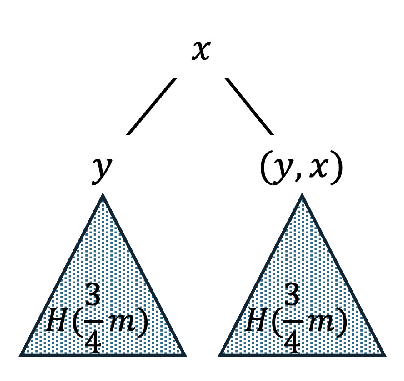
\includegraphics[scale=0.8]{fig-x_proof_tree.eps}
    \caption{$Q^{B}$における$x$の証明木で高さは,高々$H(\frac{3}{4}m)+1$である.}\label{fig-x_proof_tree}
    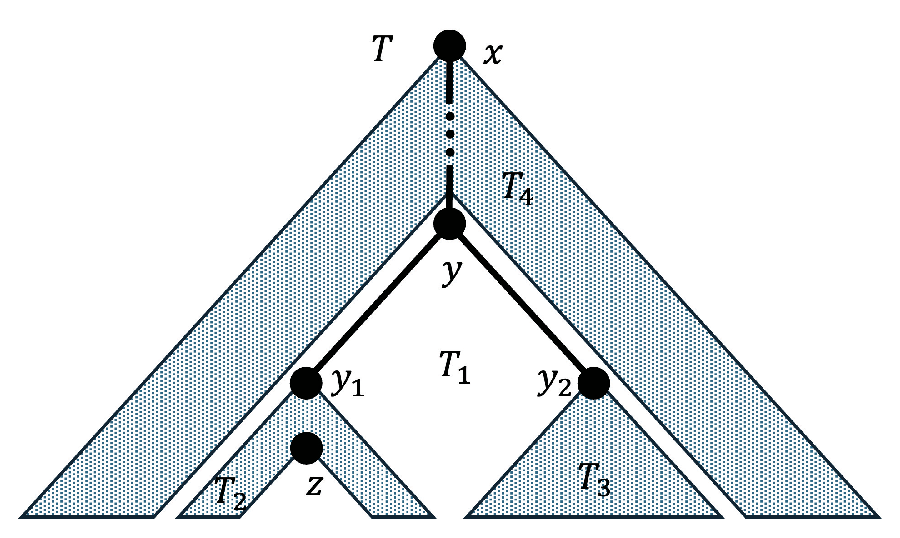
\includegraphics[scale=0.7]{fig-sub_proof_tree.eps}
    \caption{$Q$における仮定$z$での$x$の部分証明木}\label{fig:sub_proof_tree}
  \end{figure}

% 図5.2
\begin{figure}[tb]
  \centering
  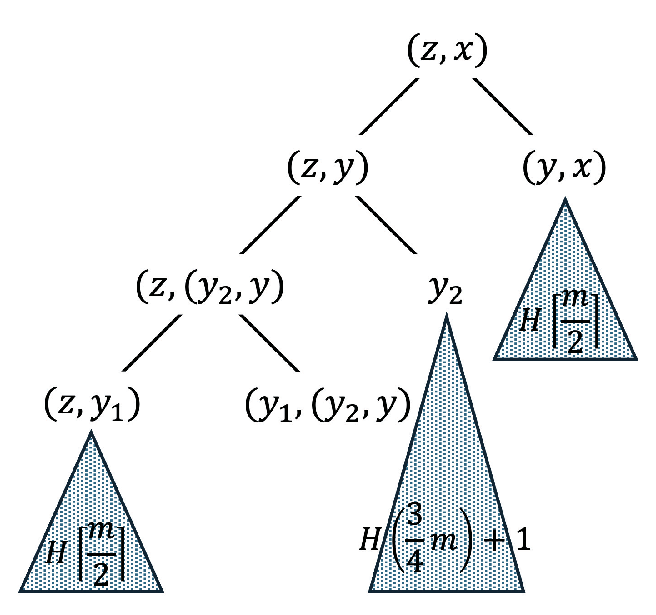
\includegraphics[scale=0.66]{fig-proof_tree.eps}
  \caption{$Q^{B}$における$(z,x)$の証明木}\label{fig:proof_tree}
\end{figure}

% 追加
\begin{proof}%[\textbf{命題\ref{prop:int0}の証明}]
  %$Q$における定理$\gamma$の証明木$T(\gamma)$に対して
  %$$height(T^{B}(\gamma))\leq 7\cdot \log(size(T(\gamma)))$$
  %を満たすバランス化推論システム$Q^{B}$における$\gamma$の証明木$T^{B}(\gamma)$が存在することを示せばよい.

  $x,y\in X$を$x\neq y$である$Q$の文とする.$Q$における仮定$y$のもとでの$x$の部分証明木とは,その根のラベルが$x$で,葉の中の1つのラベルが$y$でその他のラベルはすべて$Q$の公理であるような$Q$の推論木である.正整数$m\geq1$に対して,$S_1(m),S_2(m),H(m)$を次のように定義する.

    $S_1(m)=\{x\in X\mid Qにおけるサイズが高々mのxの証明木がある\}$,

    $S_2(m)=\{(y,x)\in X\times X\mid Qにおけるサイズが高々mの仮定yのもとでのxの部分証明木がある\}$,

    $H(m)=\max\{height_{Q^{B}}(\alpha)\mid\alpha\in S_1(m)\cup S_2(m)\}$.

  %$Q$においてサイズが1の証明木をもつものは,$Q$の公理だけであり,その証明木は根だけからなる高さが0の木である.また$S_2(1)$は空集合である.したがって$H(1)=0$である.また,$Q$においてサイズが2の証明木および仮定のもとでの部分証明木は$R$の推論規則$x\leftarrow y$から得られるものであり,このとき$(x,y)$は$Q^{B}$の公理である.したがって$H(2)=0$である.

  $m\leq 17$のとき,明らかに$H(m)\leq m$である.$m\geq 18$とし,$1\leq k\leq m-1$について$H(k)$が定まっているとする.$H(m)$に関して,次の場合を考える.
\begin{enumerate}
  \item $x\in S_1(m)$:このときサイズが高々$m$の$Q$における$x$の証明木$T$がある.系\ref{cor:1}より,$T$の頂点$y$で,$y$を根とする$T$の部分木を$T_1$とし,$T$から$T_1$の根以外の$T_1$の部分を取り除いた部分木を$T_2$とするとき,
  $$size(T_1)\leq\frac{3}{4}m, ~size(T_2)\leq\frac{3}{4}m$$
  となるものが存在する.よって,$y\in S_1(\frac{3}{4}m),(y,x)\in S_2(\frac{3}{4}m)$である.$m\geq18$のとき$m-1\geq\frac{3}{4}m$であることから$H(\frac{3}{4}m)$は定まっている.$Q^{B}$の推論規則$x\leftarrow y,(y,x)$を使い,$Q^{B}$における$x$の証明木で高さが高々$H(\frac{3}{4}m)+1$のものを構成できる(図\ref{fig-x_proof_tree}).したがって,次が成り立つ.
  $$H(m)\leq H(\frac{3}{4}m)+1$$

  \item $(z,x)\in S_2(m)$:このときサイズが高々$m$の$Q$における仮定$z$をのもとでの$x$の部分証明木$T$がある.そこで$T$の葉$z$から根$x$へ到達する道を$z$から$x$へたどっていくとき$size(T_1)>\left\lceil{\frac{size(T)}{2}}\right\rceil$となる初めての頂点を$y$とする.$T_1$を$y$を根とする$T$の部分木とする.頂点$y$の子で$y$と$z$を結ぶ道上にある頂点を$y_1$とするとき,葉$z$を含み頂点$y_1$を根とする部分木を$T_2$とする.$y$に$y_1$以外の子$y_2$があるときは,$y_2$を根とする部分木を$T_3$とする,$T_4$は$T$から$T_1$を取り除いた部分木とする(図\ref{fig:sub_proof_tree}).このとき,次の式が成り立つ.
  $$size(T_4)\leq\left\lceil{\frac{1}{2}m}\right\rceil,size(T_2)\leq\left\lceil{\frac{1}{2}m}\right\rceil, size(T_3)\leq m.$$
  図\ref{fig:proof_tree}の証明木を構成することで,$Q^{B}$における$(z,x)$の証明木ができる.したがって,次の式が成り立つ.
  $$H(m)\leq H(\frac{3}{4}m)+3.$$
\end{enumerate}

  以上の1と2から,$H(m)\leq m$ $(m\leq 17)$, $H(m)\leq H(\frac{3}{4}m)+3$ $(m\geq 18)$となり,系2より,$m=1$のとき$H(m)=1$,$m\geq 2$のとき$H(m)\leq 7\log m$が成り立つ.
\end{proof}

% 5.2
%\section{バランス化推論システムの実験的評価と今後の課題}
%最初に,二分化された順序木に対する均衡化について述べる.ページ数の都合上,二分線形順序項木パターンに対する均衡化の詳細は省略する.順序木$T=(V_T,E_T)$を変数集合が空である線形順序項木パターンとみなし,
二分化を行った順序木\cite{miyano-parallel1993}または子の数の最大値2の無順序木を,その構造の情報を保ったままバランス化が可能である.
%を$B(T)$とする.次のように$B(T)$を均衡化する.二分均衡化された$B(T)$の任意の頂点は高々2頂点を子として持つ.最初に,$B(T)$の頂点の頂点識別子$\alpha_0$とその子の頂点識別子 $\alpha_1,\alpha_2$の関係を「公理」とみなす.
%\begin{eqnarray*}
%  S_0&=&\{\alpha_0\mid\alpha は子を持たない\},\\
%  S_1&=&\{(\alpha_1,\alpha_0)\mid\alpha_0は唯一つの子\alpha_1を持つ\},\\
%  S_2&=&\{(\alpha_2,(\alpha_1,\alpha_0)),(\alpha_1,(\alpha_2,\alpha_0))\mid\alpha_0は2つの子\alpha_1と\alpha_2を持つ\}
%\end{eqnarray*}
%$S=S_0\cup S_1\cup S_2$として,これを$B(T)$の公理集合と呼ぶ.頂点数$N$の順序木$T$に対して,$B(T)$の頂点数が2$N-1$であることから,$\abs{S}\leq 4N$である.この公理の集合に対して,次の3つの推論規則を用いて,$B(T)$の根の頂点識別子($T$の根の頂点識別子でもある)に対する証明木を構築する.
%\begin{eqnarray*}
%  x&\leftarrow&y,(y,x)\\
%  (y,x)&\leftarrow&z,(z,(y,x))\\
%  (z,x)&\leftarrow&(z,y),(y,x)
%\end{eqnarray*}
%本研究では更に以下の証明木を提案する.
%\begin{eqnarray*}
%  (z,(y,x))&\leftarrow&(z,w),(w,(y,x))\\
%  (z,x)&\leftarrow&y,(z,(y,x))
%\end{eqnarray*}
%
%頂点数$N$の順序木$T$に対する$B(T)$の証明木を,$N$の多項式サイズのプロセッサを持つPRAMにより$O(\log N)$時間で計算できることが,宮野\cite{miyano-parallel1993}のテキストp.252により示されている.また,同テキストp.246の命題8.2の証明を訂正することにより,頂点数$N$が6以上の順序木$T$に対して,高さが高々5$\log N$であるような証明木を構築できることが示される.高さが高々5$\log N$である$B(T)$の証明木のひとつを$B(T)^Q$とする.
$\log m$の係数7は理論的解析により得られたもので,実際には,図\ref{fig:binary}のように頂点数18以下の全ての順序木に対して,高さが高々2$\log m$の証明木が存在する.$m\geq 18$のとき,$\log m$の係数を理論的に7未満にできるか否かは未解決である.

%次に,動的計画法を用いて,$B(T)^Q$の各頂点$x$の深さの降順に,頂点$x$に対応可能な$B(t)$の証明木の頂点の集合(CS($x$)と記す)を決定する.より具体的には,$B(T)^Q$の各頂点$x$に対して,二分線形順序項木パターン$B(t)$の公理集合と上記の推論規則,さらに変数に依存した継承規則を用いて,あらかじめ計算された$x$の高々2つの子$y,z$のCS($y$)とCS($z$)からCS($x$)を決定する.$B(T)^Q$の同じ深さの頂点$x$に対しては並列にCS($x$)を計算できるので,計算時間は$B(T)^Q$の高さに依存する.以上より,次の定理を得る.証明は省略する.

% 図5.3
\begin{figure}[tb]
  \centering
  \includegraphics[scale=0.7]{binary.eps}
  \caption{頂点数とバランス化後の木の高さの解析}\label{fig:binary}
\end{figure}

% 5.3
%\section{今後の課題}
%並列ランダムアクセス機械(Parallel Random Access Machine,PRAMと略す)とは,共有メモリをプロセッサ間の通信手段とする並列計算の理論的モデルである\cite{greenlaw-parallel1995}\cite{miyano-parallel1993}.効率のよい並列アルゴリズムとは,入力サイズ$n$に対して,$O(n^k)$個のプロセッサを持つPRAM上で,$O((\log n)^{c})$時間で計算するアルゴリズム(ただし$k$と$c$は$n$に依存しない定数)のことをいう.効率のよい並列アルゴリズムを持つ計算問題のクラスをNC(Nick's Class)という.クラスPに含まれる計算問題がいつでもNCに含まれるかという問いは並列計算量理論における未解決問題である.財津[4]は,推論システムのバランス化を用いて,線形順序項木パターンと順序木を入力とするパターン照合問題に対して,効率の良い並列アルゴリズムを提案した.しかし,そのアルゴリズムは,\cite{miyano-parallel1993}の補題8.1(p.246)の誤りにより正しい並列計算量が得られない.そこで本章では,新しい推論規則とそれを用いる推論システムのバランス化を提案して,線形順序項木パターンと順序木,または子の数の最大値2の線形無順序項木パターンと無順序木を入力とするパターン照合問題の効率の良い並列アルゴリズムの設計と解析に対する基盤とする.

%の二分バランス化手法を提案した.本論文では,同テキスト\cite{miyano-parallel1993}中に示された推論の並列化手法の高さの見積りに関する証明の誤りを訂正た.
%し,実際に,頂点数$n$の線形順序項木パターンと頂点数$N$の順序木を,それぞれ高さ$O(\log n)$の線形順序項木パターンと高さ$O(\log N)$の順序木に変換できることを示す.さらに,線形順序項木パターン照合問題に対する並列アルゴリズム提案し,その並列アルゴリズムがPRAM上で,頂点数$n$の線形順序項木パターンと頂点数$N$の順序木に対して,$n$と$N$の多項式個のプロセッサを用いて,$O(\log n)$時間で解くことができることを示す.

%\section{二分線形順序項木パターン(今後の課題に)}
%$t=(V_t,E_t,H_t)$を線形順序項木パターンとする.以下では,$t$の頂点には,その頂点を識別する固有の番号または記号(列)が与えられているものとする.その番号を頂点識別子と呼び,$u\in V_t$に対して,$\langle u\rangle$で表す.同様に,$t$の辺と変数にも,それぞれ互いに異なる辺識別子と変数識別子が与えられており,各$(u_0,u_1)\in E_t$と$[u_0,u_1]\in E_t$に対して,同じ記号$\langle u_0,u_1 \rangle$で表す.$t$の任意の頂点$u_0$の子を兄弟の順に$u_1,u_2,\ldots,u_\ell(\ell\geq 0)$とし,$u_0$に対して,
%\begin{eqnarray*}
%  V_{B(t)}^{n_0}&=&\{\langle u_0\rangle,\langle u_1\rangle,\ldots,\langle u_\ell\rangle\}\cup\{\langle u_0,u_1\rangle,\ldots,\langle u_0,u_\ell\rangle\},\\
%  H_{B(t)}^{n_0}&=&\{(\langle u_0\rangle,\langle u_0,u_\ell\rangle),(\langle u_0,u_\ell\rangle,\langle u_\ell\rangle),(\langle u_0,u_\ell\rangle,\langle u_0,u_{\ell-1}\rangle)\mid[u_0,u_\ell]\in H_T\}\\
%  &\cup&\{(\langle u_0,u_{i+1}\rangle,\langle u_0,u_i\rangle),(\langle u_0,u_i\rangle,\langle u_i\rangle),(\langle u_0,u_i\rangle,\langle u_0,u_{i-1}\rangle)\mid[u_0,u_i]\in H_T,1<i<\ell\}\\
%  &\cup&\{(\langle u_0,u_2\rangle,\langle u_0,u_1\rangle),(\langle u_0,u_1\rangle,\langle u_1\rangle)\mid[u_0,u_1]\in H_T\},\\
%  E_{B(t)}^{n_0}&=&\{(\langle u_0\rangle,\langle u_0,u_\ell\rangle),(\langle u_0,u_i\rangle,\langle u_i\rangle),(\langle u_0,u_{i+1}\rangle,\langle u_0,u_i\rangle)\mid1\leq i\leq\ell\}\setminus H_{B(t)}^{u_0}
%\end{eqnarray*}
%とおく.$t$の二分線形順序項木パターンを
%\begin{eqnarray*}
%  B(t)=(\bigcup_{u_0\in V_t}V_{B(t)}^{u_0},\bigcup_{u_0\in V_t}E_{B(t)}^{u_0},\bigcup_{u_0\in V_t}H_{B(t)}^{u_0})
%\end{eqnarray*}
%とする.$B(t)$の頂点識別子で表される頂点$\langle u\rangle$を実頂点,辺識別子と変数識別子で表される頂点$\langle u,u'\rangle$を仮頂点と呼ぶ.図2に線形順序項木パターン$t$と二分線形順序項木パターン$B(t)$の例を示す.$n$頂点の線形順序項木パターン$t$に対して,二分線形順序項木パターン$B(t)$の頂点数は$2n-1$となる.

% 6 結論
% 6
%\chapter{結論}
\section{まとめと今後の課題}
本論文では,線形無順序木パターンに対する質問学習モデルのオラクルとしてグラフ畳み込みネットワーク(Graph Convolutional Network, GCN)を採用した新たな質問学習モデルを提案した.このモデルは,従来の完全な教師(オラクル)を仮定した手法とは異なり,高精度な深層学習モデルであるGCNを活用し,データの構造的特徴を効率的に発見することを目的としている.さらに,本研究では,質問学習モデルで使用されるアルゴリズムについて検討を行い,既存手法よりも高速な処理を可能とする新たなアルゴリズムを提案した.

第1章では,まず背景として,近年,グラフ構造を持つデータが飛躍的に増加しており,これらのデータを活用した研究が盛んに行われている現状について述べた.これらのデータ活用手法の一つとして,本研究ではGCNに注目した.GCNは,グラフ構造データを対象とした機械学習手法であり,高精度な分類が可能であることが報告されている.また,計算論的学習理論における機械学習モデルの一つである質問学習にも着目した.質問学習モデルの中でも,本研究では,学習対象が目標概念に属すか否かを$Yes$または$No$で応答する所属性質問を利用した.この両手法を順序項木パターンに応用した先行研究として,小田ら\cite{oda-ai2022}による研究があることを述べた.この研究では,順序木データを対象にGCNを用いて学習を行い,さらにそのGCNの予測根拠を質問学習モデルを通じて順序項木パターンとして明らかにする手法を提案し,実験的にその有効性を示している.本研究では,対象を無順序木に拡張し,(1)二値分類問題,(2)無矛盾性問題,(3)可視化問題の3つの計算問題を解析することで,GCNと質問学習モデルを統合した協調モデルの有効性を示すことを目的とした.さらに,質問学習モデルにおけるアルゴリズムについても検討を行い,既存手法に比べて高速な処理を可能とする新たなアルゴリズムを提案した.

第2章では,本研究の準備として,本論文で使用する基本的な用語と概念を整理した.離散数学におけるグラフは,頂点集合を$V$,辺集合を$E$とするとき,$G=(V,E)$で表される集合構造である.本研究では,グラフの一種である木を対象とし,特別な頂点である根(root)を1つ持ち,閉路を含まない構造としての根付き木に注目した.木は,性質に基づいて大きく2つの種類に分類される.一つは,兄弟関係を持たず,子の順序が定義されていない無順序木であり,もう一つは,兄弟関係を持ち,子の順序が明確に定義される順序木である.

第3章では,線形無順序木パターンを質問学習に適応する方法について述べた.まず,線形無順序木パターンに関連する計算問題の計算量について議論し,照合問題(${\cal LUTP}$-${\cal MP}$)と無矛盾性問題(${\cal LUTP}$-${\cal CP}$)がNP完全であることを示した.これらの証明は,充足可能性問題(3-SAT)からそれぞれの問題への多項式時間帰着を構築することで行った.次に,Amoth\cite{amoth-ml2001}によって提案されたアルゴリズムを基に,線形無順序木パターンの同定を可能とする新たなアルゴリズム${\cal LUTP}$-${\cal QUERY}_{{\cal O}(t)}^{Square}$を提案した.このアルゴリズムは,入力として与えられる無順序木の頂点数を$N$とした場合,$O(N^2)$回の所属性質問を用いて元の線形無順序木パターンを同定可能である.さらに,計算効率を向上させるため,$O(N)$回の所属性質問で同定を実現するアルゴリズム${\cal LUTP}$-${\cal QUERY}_{{\cal O}(t)}^{Linear}$を提案した.これらのアルゴリズムについて理論的解析および計算機実験を通じて詳細に検証し,その正当性と有効性を証明した.

第4章では,本論文のタイトルにも示されている,線形無順序木パターンに対するグラフ畳み込みネットワーク(GCN)をオラクルとする質問学習モデルについて述べた.まず,GCNの学習に使用するPythonの機械学習ライブラリであるPyTorch Geometric(PyG)に実装されている畳み込み層であるGCNConv,GraphConv,RGCNConvについて,それぞれの畳み込み方法の違いを数式を用いて説明した.これらのグラフ畳み込み層を利用して,GCNをオラクルとする線形無順序木パターンに対する所属性質問を提案した.この手法では,質問学習モデルにおける完全な教師(オラクル)をGCNに置き換えることで,協調モデルを構築する.この協調モデルは,不完全な教師である場合でも,元の線形無順序木パターンを発見することを目的としている.次に,提案する協調モデルの有効性を確認するための計算機実験について述べた.評価は,データセット$S$を対象として以下の3つの計算問題に基づき,F値を用いて行った.(1)二値分類問題:無順序木の特徴量を用いて,データセット$S$に属す無順序木が元のクラスに分類可能かを検証する.(2)無矛盾性問題:データセット$S$をクラス分類するための線形無順序木パターンが存在するか否かを決定する.(3)可視化問題:一般にブラックボックスである深層学習モデルの予測根拠を,線形無順序木パターンを用いて明らかにする.実験結果から,非常に高い精度でデータセットを分類するGCNを学習できることが確認された.しかし,新しいデータセットに対しては,学習データとの差が大きく,過学習が発生している可能性が示唆された.一方で,提案する協調モデルは高い精度で分類する線形無順序木パターンを一定程度発見できた.これは,学習データと新しいデータセット間の差が小さく,協調モデルが過学習を起こしにくいことを示している.さらに,グラフ畳み込み層と質問学習アルゴリズムの性能の違いを検討した.結果として,GraphConvを使用した場合はアルゴリズム${\cal LUTP}$-${\cal QUERY}_{{\cal O}(t)}^{Square}$の精度が高く,RGCNConvを使用した場合はアルゴリズム${\cal LUTP}$-${\cal QUERY}_{{\cal O}(t)}^{Linear}$の精度が高いことが確認された.これは,GraphConvが隣接する頂点数に基づいて特徴を集約するのに対し,RGCNConvが辺ラベルの種類に基づいて特徴を集約するという両者の特性の違いによる結果であると考察した.さらに,計算機実験ではランダムに生成した線形無順序木パターンを用いており,協調モデルによって出力される線形無順序木パターンの精度が高いものと低いものが存在することが確認された.そこで,精度と各要素間の相関関係について調査を行ったが,いずれの結果にも有意な相関は見られなかった.

今後の課題として,協調モデルに対して無順序木の項木パターンへの拡張が挙げられる.東山ら\cite{higashiyama-hinokuni2024}は,順序木に内部変数を含む線形順序項木パターンを用いた協調モデルを提案し,非常に高精度なデータ分類を実現する線形順序項木パターンの獲得に成功している.しかし,この方法を線形無順序項木パターンに適用するためには,新たな課題を解決する必要がある.無順序木は兄弟関係に順序がない特性を持つため,従来のアルゴリズムや本研究で提案した${\cal LUTP}$-${\cal QUERY}_{{\cal O}(t*)}^{Linear}$などのアルゴリズムをそのまま使用することは困難である.この特性により,内部変数を含む線形無順序項木パターンの構造を効率的に扱うアルゴリズムの設計が極めて難しい.したがって,無順序木の特性を踏まえた新たな質問学習アルゴリズムの開発が不可欠である.またそれに加え,実世界で得られるグラフデータに対して,本研究で提案したグラフ畳み込みネットワーク(GCN)と質問学習モデルの協調モデルを適用し,具体的なパターン発見手法を確立することがあげられる.この際,グラフデータの複雑な構造を表現する手段として,形式グラフ文法や形式グラフ体系をグラフパターンの記述手法として採用することが有効であると考えられる.さらに,それらを活用したGCNと質問学習モデルの協調モデルを設計・解析し,実世界の多様なグラフデータにおけるパターン発見の精度向上や新たな知見の抽出に寄与することがあげられる.


% 7 参考文献
\begin{thebibliography}{99}

  % 1
  \bibitem{angluin-ml1988}
  Angluin, D.:
  Queries and Concept Learning,
  Matching Learning, Vol.2, No.4, pp.319--342 (1988).

  % 2
  \bibitem{angluin-jcss1980}
  Angluin, D.:
  Finding patterns common to a set of strings,
  Journal of Computer and System Sciences, Vol.21, No.1, pp.46-62 (1980).

  % 3
  \bibitem{angluin-ic1987}
  Angluin, D.:
  Learning Regular Sets from Queries and Counterexamples,
  Information and Computation, Vol.75, No.2, pp.87-106 (1987).

  \bibitem{amoth-ml2001}
  Amoth, T.R., Cull, P., Tadepalli, P.:
  On Exact Learning of Unordered Tree Patterns,
  Machine Learning, Vol.44, pp211-243 (2001).

  \bibitem{greenlaw-parallel1995}
  Greenlaw, R., Hoover, H.J., and Ruzzo, W.L.:
  Limits to Parallel Computation: P-Completeness Theory, 
  Oxford University Press (1995).

  \bibitem{higashiyama-hinokuni2024}
  東山 的生, 内田 智之, 正代 隆義, 松本 哲志:
  順序項木パターンに対する学習済GCNをオラクルとした質問学習アルゴリズムのランダム化による精度向上,
  情報処理学会九州支部火の国情報シンポジウム講演論文集, B6-1, pp.1--6 (2024).

  \bibitem{pyg-gcnconv}
  Kipf, T. N. and Welling, M.: 
  Semi-Supervised Classification with Graph Convolutional Networks, 
  Proc. ICLR 2017, arXiv:1609.02907 (2017).

  \bibitem{matsumoto-ieice2020}
  Matsumoto, S., Uchida, T., Shoudai, T., Suzuki, Y., and Miyahara, T.:
  An Efficient Learning Algorithm for Regular Pattern Languages Using One Positive Example and a Linear Number of Membership Queries,
  IEICE Transactions on Information and Systems, Vol.E103-D, No.3, pp.526-539 (2020).

  %\bibitem{miyano-parallel1993}
  %宮野 悟:
  %並列アルゴリズム,
  %近代科学社 (1993).

  \bibitem{miyano-ngc2000}
  Miyano,~S., Shinohara,~A. and Shinohara,~T.:
  Polynomial-time Learning of Elementary Formal Systems,
  New Generation Computing, Vol.18, pp.217--242 (2000).

  \bibitem{pyg-graphconv}
  Morris, C. et al.: 
  Weisfeiler and Leman Go Neural: Higher-Order Graph Neural Networks, 
  Proc. AAAI Conference on Artificial Intelligence, 
  Vol.33, No.1, pp.4602-4609 (2019). 

  \bibitem{nii-nakano_uno2003}
  Nakano, S. and Uno, T.:
  Efficient generation of rooted trees,
  National Institute for Informatics (Japan),
  Tech. Rep. NII-2003-005E 8,
  pp.4--63, (2003).

  \bibitem{cs-nakano_uno2004}
  Nakano, S. and Uno, T.:
  Constant Time Generation of Trees with Specified Diameter, Graph-Theoretic Concepts in Computer Science (WG2004),
  LNCS 3353, pp.33-45 (2004).

  \bibitem{oda-ai2022}
  小田 直季, 内田 智之, 正代 隆義, 松本 哲志, 鈴木 祐介, 宮原 哲浩:
  順序木パターンの質問学習アルゴリズムによるグラフ畳み込みネットワークの予測根拠の可視化,
  2022年度人工知能学会全国大会(第36回), 2G4-GS-2-01 (2022).

  \bibitem{pyg-rgcnconv}
  Schlichtkrull, M. et al.: 
  Modeling Relational Data with Graph Convolutional Networks, 
  The Semantic Web, ESWC 2018, LNCS 10843, pp.593--607 (2018). 

  \bibitem{shoudai-ieice2018}
  Shoudai,~T., Miyahara,~T., Uchida,~T., Matsumoto,~S., and Suzuki,~Y.:
  An Efficient Pattern Matching Algorithm for Unordered Term Tree Patterns of Bounded Dimension,
  IEICE Trans. Fundamentals, Vol.E101-A, No.9, pp.1344--1354 (2018).

  \bibitem{suzuki-tcs2006}
  Suzuki, Y., Shoudai, T., Uchida, T., and Miyahara, T.:
  Ordered term tree languages which are polynomial time inductively inferable from positive data,
  Theoretical Computer Science, Vol.350, pp.63-90 (2006).

  \bibitem{uchida2014}
  Uchida, T., Matsumoto, S., Okada, R., Shoudai, T., Suzuki, Y., and Miyahara, T.:
  Exact Learning of Finite Unions of Graph Patterns from Queries,
  Journal of Information Processing, Vol.22, No.1, pp.1--8 (2014).

  \bibitem{uchida-ieice2019}
  Uchida, T., Matsumoto, S., Shoudai, T., Suzuki, Y., and Miyahara, T.:
  Exact Learning of Primitive Formal Systems Defining Labeled Ordered Tree Languages via Queries,
  IEICE Transactions on Information and Systems, Vol.E102-D, No.3, pp.470-482 (2019).

  %\bibitem{zaitsu}
  %財津 恭太:
  %順序項木パターンに対するNCマッチングアルゴリズム,
  %平成14年度九州大学大学院システム情報科学府修士論文 (2003).


\end{thebibliography}

% ファイリングしている参考文献を載せる

% 謝辞
\chapter*{謝辞}
\addcontentsline{toc}{chapter}{謝辞}
\thispagestyle{empty}
本研究の遂行にあたり,指導教員として終始多大なるご指導とご助言を賜りました正代隆義教授に,心より深く感謝申し上げます.
また,本論文の作成に際し,副査として適切なご助言を頂きました馬場謙介教授ならびに宮田考史准教授に,厚く御礼申し上げます.
広島市立大学の内田智之教授と東海大学の松本哲志教授には,オンラインゼミを通じて大変有意義なコメントを賜りました.ここに深く感謝の意を表します.
最後に,情報工学科の教職員の皆様には,多岐にわたり貴重なご助言を頂きましたことに感謝いたします.

% 研究業績
\chapter*{研究業績}
\addcontentsline{toc}{chapter}{研究業績}
\thispagestyle{empty}

\section*{国内会議発表}
\begin{itemize}
  \item \uline{石灘洸樹},正代隆義,内田智之,松本哲志,超高精度グラフ畳み込みネットワークをオラクルとする無順序木パターンの質問学習モデル,情報処理学会 第85回全国大会講演論文集,pp373-374(2023)
  \item \uline{石灘洸樹},正代隆義,内田智之,松本哲志,無順序木パターンに対する高精度グラフ畳み込みネットワークをオラクルとする質問学習モデルの解析,研究報告数理モデル化と問題解決(MPS),Vol.2023-MPS-143,No.15,pp.1-8(2023)
  \item \uline{石灘洸樹},正代隆義,内田智之,互いに異なる変数ラベルを持つ順序木構造パターンに対する効率のよい並列アルゴリズム,第76回電気・情報関係学会九州支部連合大会論文集,pp.289-290(2023)
  \item \uline{石灘洸樹},正代隆義,内田智之,松本哲志,線形回数の所属性質問と1つの正例による無順序木パターン言語族に対する質問学習アルゴリズム,情報科学技術フォーラム講演論文集,pp.77-82(2024)
\end{itemize}

\end{spacing}

\end{document}